%%%%%%%%%%%%%%%%%%%%%%%%%%%%%%%%%%%%%%%%%
% Beamer Presentation
% LaTeX Template
% Version 1.0 (10/11/12)
%
% This template has been downloaded from:
% http://www.LaTeXTemplates.com
%
% License:
% CC BY-NC-SA 3.0 (http://creativecommons.org/licenses/by-nc-sa/3.0/)
%
%%%%%%%%%%%%%%%%%%%%%%%%%%%%%%%%%%%%%%%%%

%----------------------------------------------------------------------------------------
%	PACKAGES AND THEMES
%----------------------------------------------------------------------------------------

\documentclass{beamer}

\mode<presentation> {

% The Beamer class comes with a number of default slide themes
% which change the colors and layouts of slides. Below this is a list
% of all the themes, uncomment each in turn to see what they look like.

\usetheme{default}

\usecolortheme{seahorse}


%packages for changing the size of the only slide
\usepackage{changepage}
\usepackage{lipsum}
\usepackage{textpos}

\usepackage{bbding}
\usepackage{pifont}
\usepackage{wasysym}
\usepackage{amssymb}

%\setbeamertemplate{footline} % To remove the footer line in all slides uncomment this line
%\setbeamertemplate{footline}[page number] % To replace the footer line in all slides with a simple slide count uncomment this line

%\setbeamertemplate{navigation symbols}{} % To remove the navigation symbols from the bottom of all slides uncomment this line
}

\usepackage{graphicx} % Allows including images
\usepackage{booktabs} 

\usepackage{graphicx} % Allows including images
\usepackage{booktabs} % Allows the use of \toprule, \midrule and \bottomrule in tables

\usepackage{xcolor}

\definecolor{OliveGreen}{cmyk}{0.70,0,0.95,0.30}





\usepackage{media9}
\usepackage{multimedia,chemfig}
\newcommand{\xmark}{\ding{55}}%
%----------------------------------------------------------------------------------------
%	TITLE PAGE
%----------------------------------------------------------------------------------------

\title[Models for phosphomembranes]{Dynamics of membrane bound peptides from NMR experiments and MD simulations} % The short title appears at the bottom of every slide, the full title is only on the title page

\author[Ricky Nencini]{Ricky Nencini\\ \small Supervisor: Samuli Ollila} % Your name
\institute[IOCB] % Your institution as it will appear on the bottom of every slide, may be shorthand to save space
{
Faculty of Science, University of Helsinki\\
Institute of Biotechnology \\ 
\includegraphics[height=1.5cm]{pictures/Carolinum_Logo.pdf} \hspace{0.1cm}
\includegraphics[height=1.5cm]{pictures/logo.eps} \hspace{0.1cm}  % Your institution for the title page
\includegraphics[height=1.5cm]{pictures/logo_nature.pdf} \\
\medskip
\textit{ricky.nencini@helsinki.fi} % Your email address
}
\date{\today} % Date, can be changed to a custom date

\addtobeamertemplate{navigation symbols}{}{%
    \usebeamerfont{footline}%
    \usebeamercolor[fg]{footline}%
    \hspace{1em}%
    \insertframenumber/\inserttotalframenumber
}
\usefonttheme[onlymath]{serif}
\setbeamertemplate{frametitle}[default][center]
\begin{document}
\def\inserttotalframenumber{28}

\section{Intro}




\begin{frame}
\titlepage % Print the title page as the first slide
\end{frame}


%%%%%%%%%%%%%%%%%%%%%
%Set logo to every title
%%%%%%%%%%%%%%%%%%%%%
%\addtobeamertemplate{frametitle}{}{%
%\begin{textblock*}{100mm}(0.98\textwidth,-1cm)
%\includegraphics[height=1cm]{pictures/logo.eps}
%\end{textblock*}}

\subsection{Goal}






\begin{frame}
\begin{center}
\Large{\centering
\textbf{Goal: What can we tell about membrane proteins based on differences in spin relaxation times?} \\}

\vspace{0.5cm}


\includegraphics[height=5cm]{can_we0.pdf}
\end{center}
\end{frame}

\addtocounter{framenumber}{-1}
\begin{frame}
\begin{center}
\Large{\centering
\textbf{Goal: What can we tell about membrane proteins based on differences in spin relaxation times?} \\}

\vspace{0.5cm}

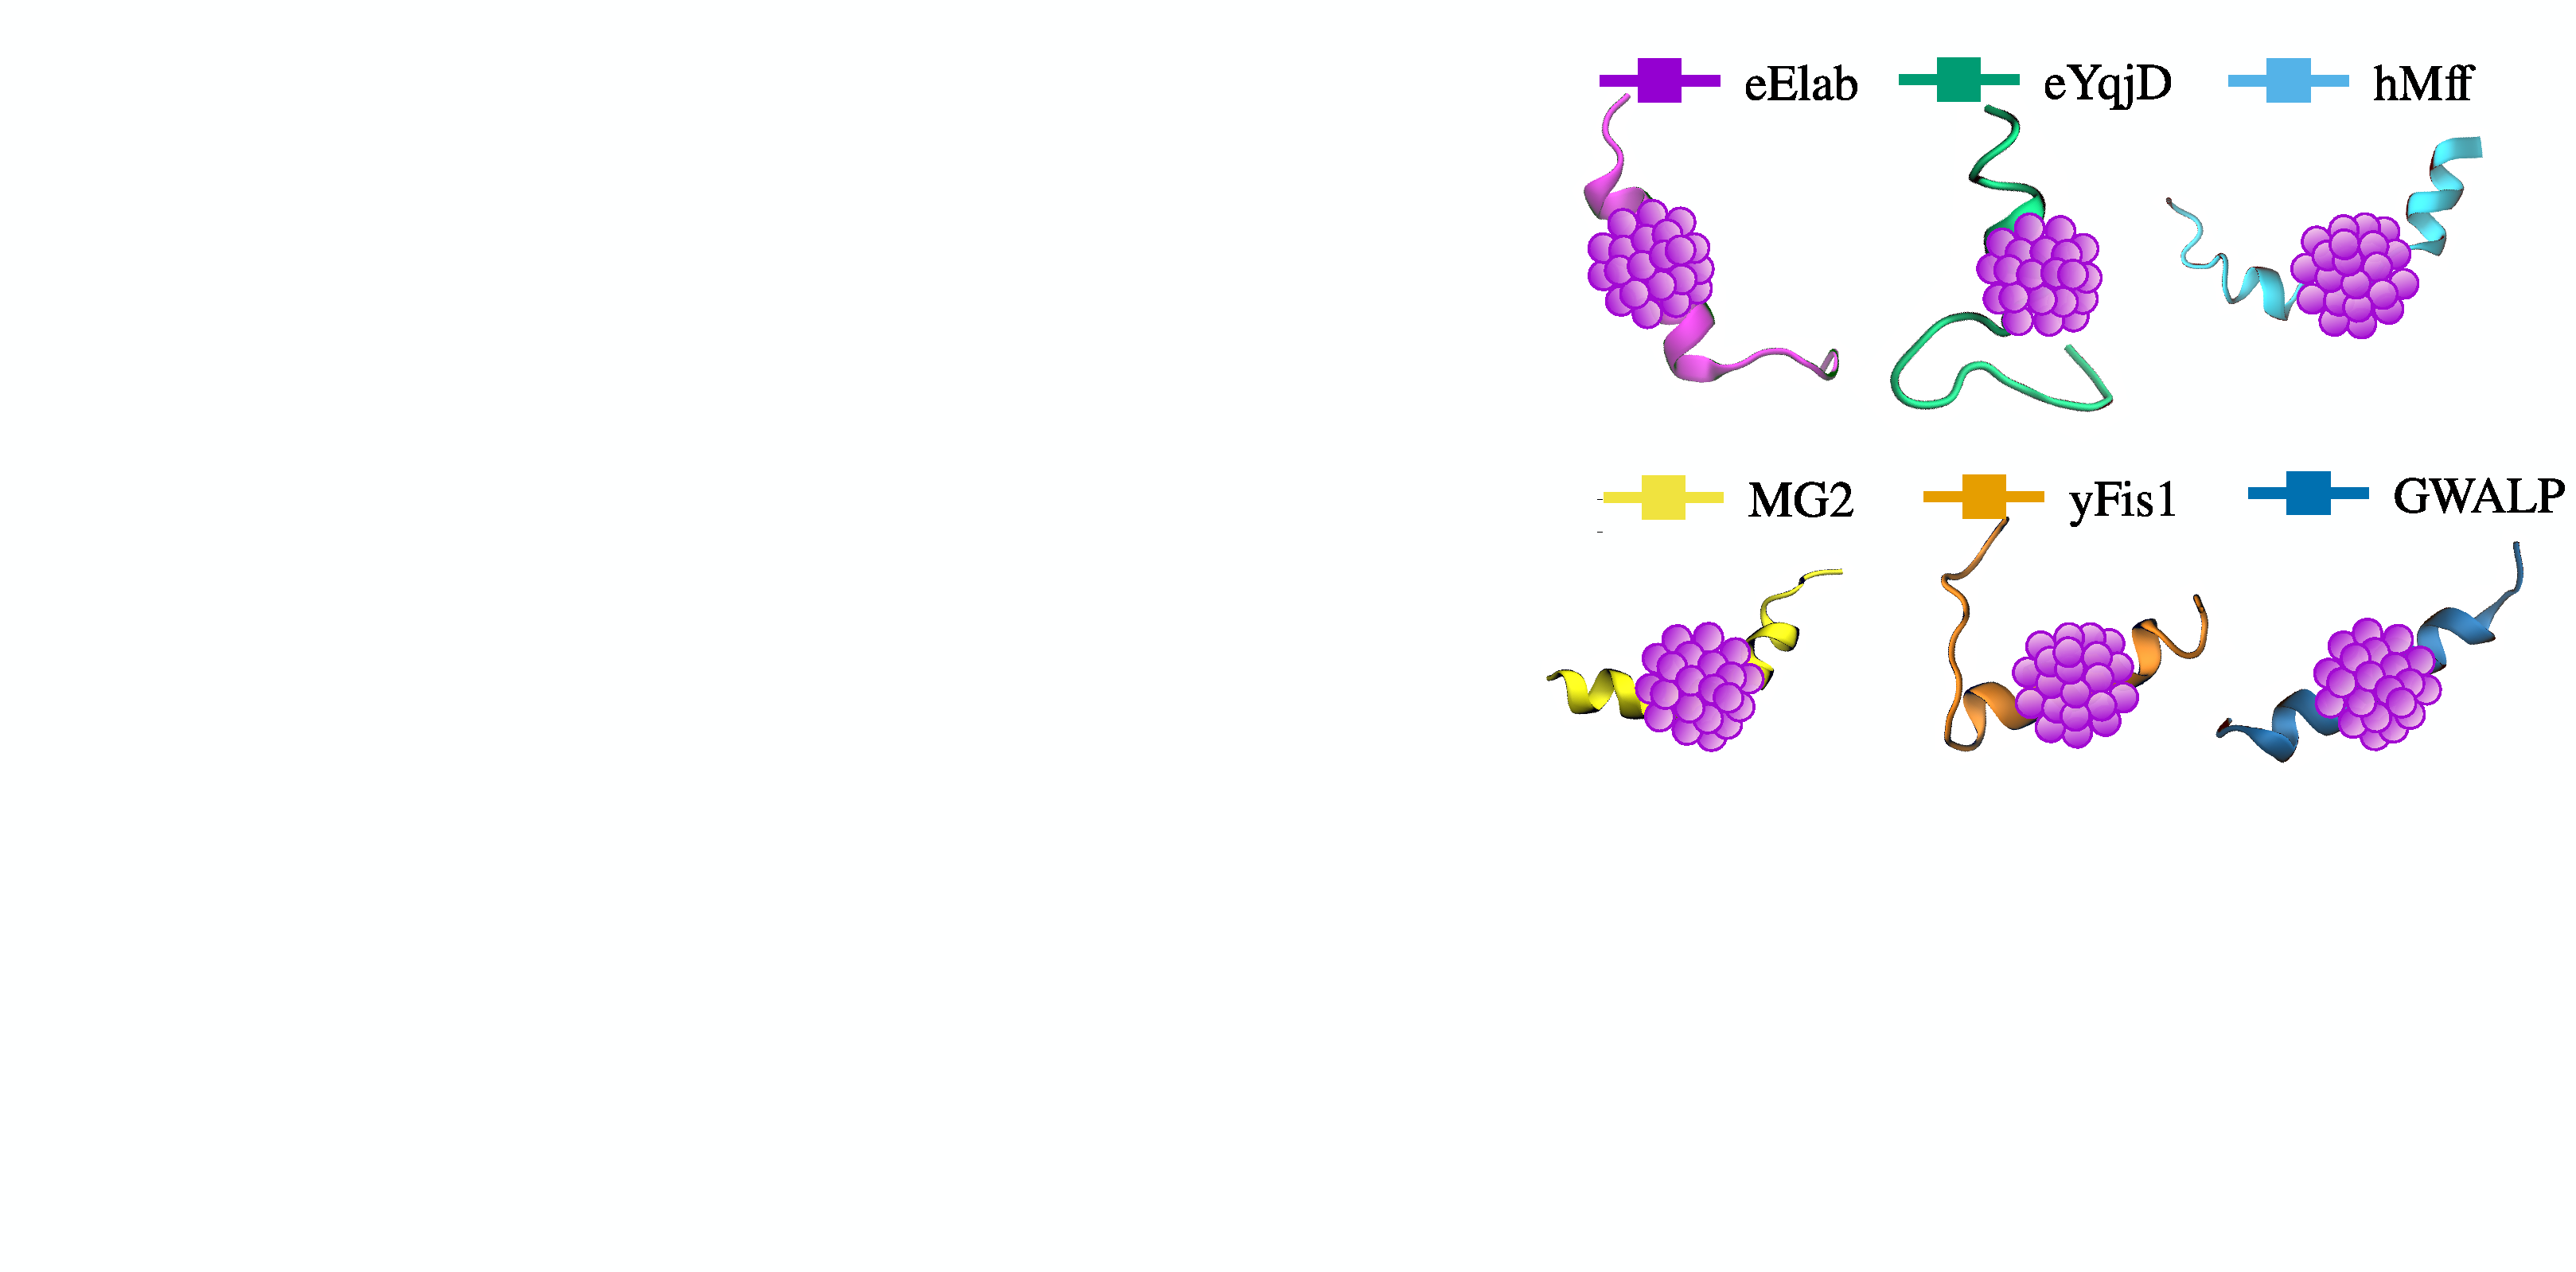
\includegraphics[height=5cm]{can_we1.pdf}
\end{center}
\end{frame}

\addtocounter{framenumber}{-1}
\begin{frame}
\begin{center}
\Large{\centering
\textbf{Goal: What can we tell about membrane proteins based on differences in spin relaxation times?} \\}

\vspace{0.5cm}

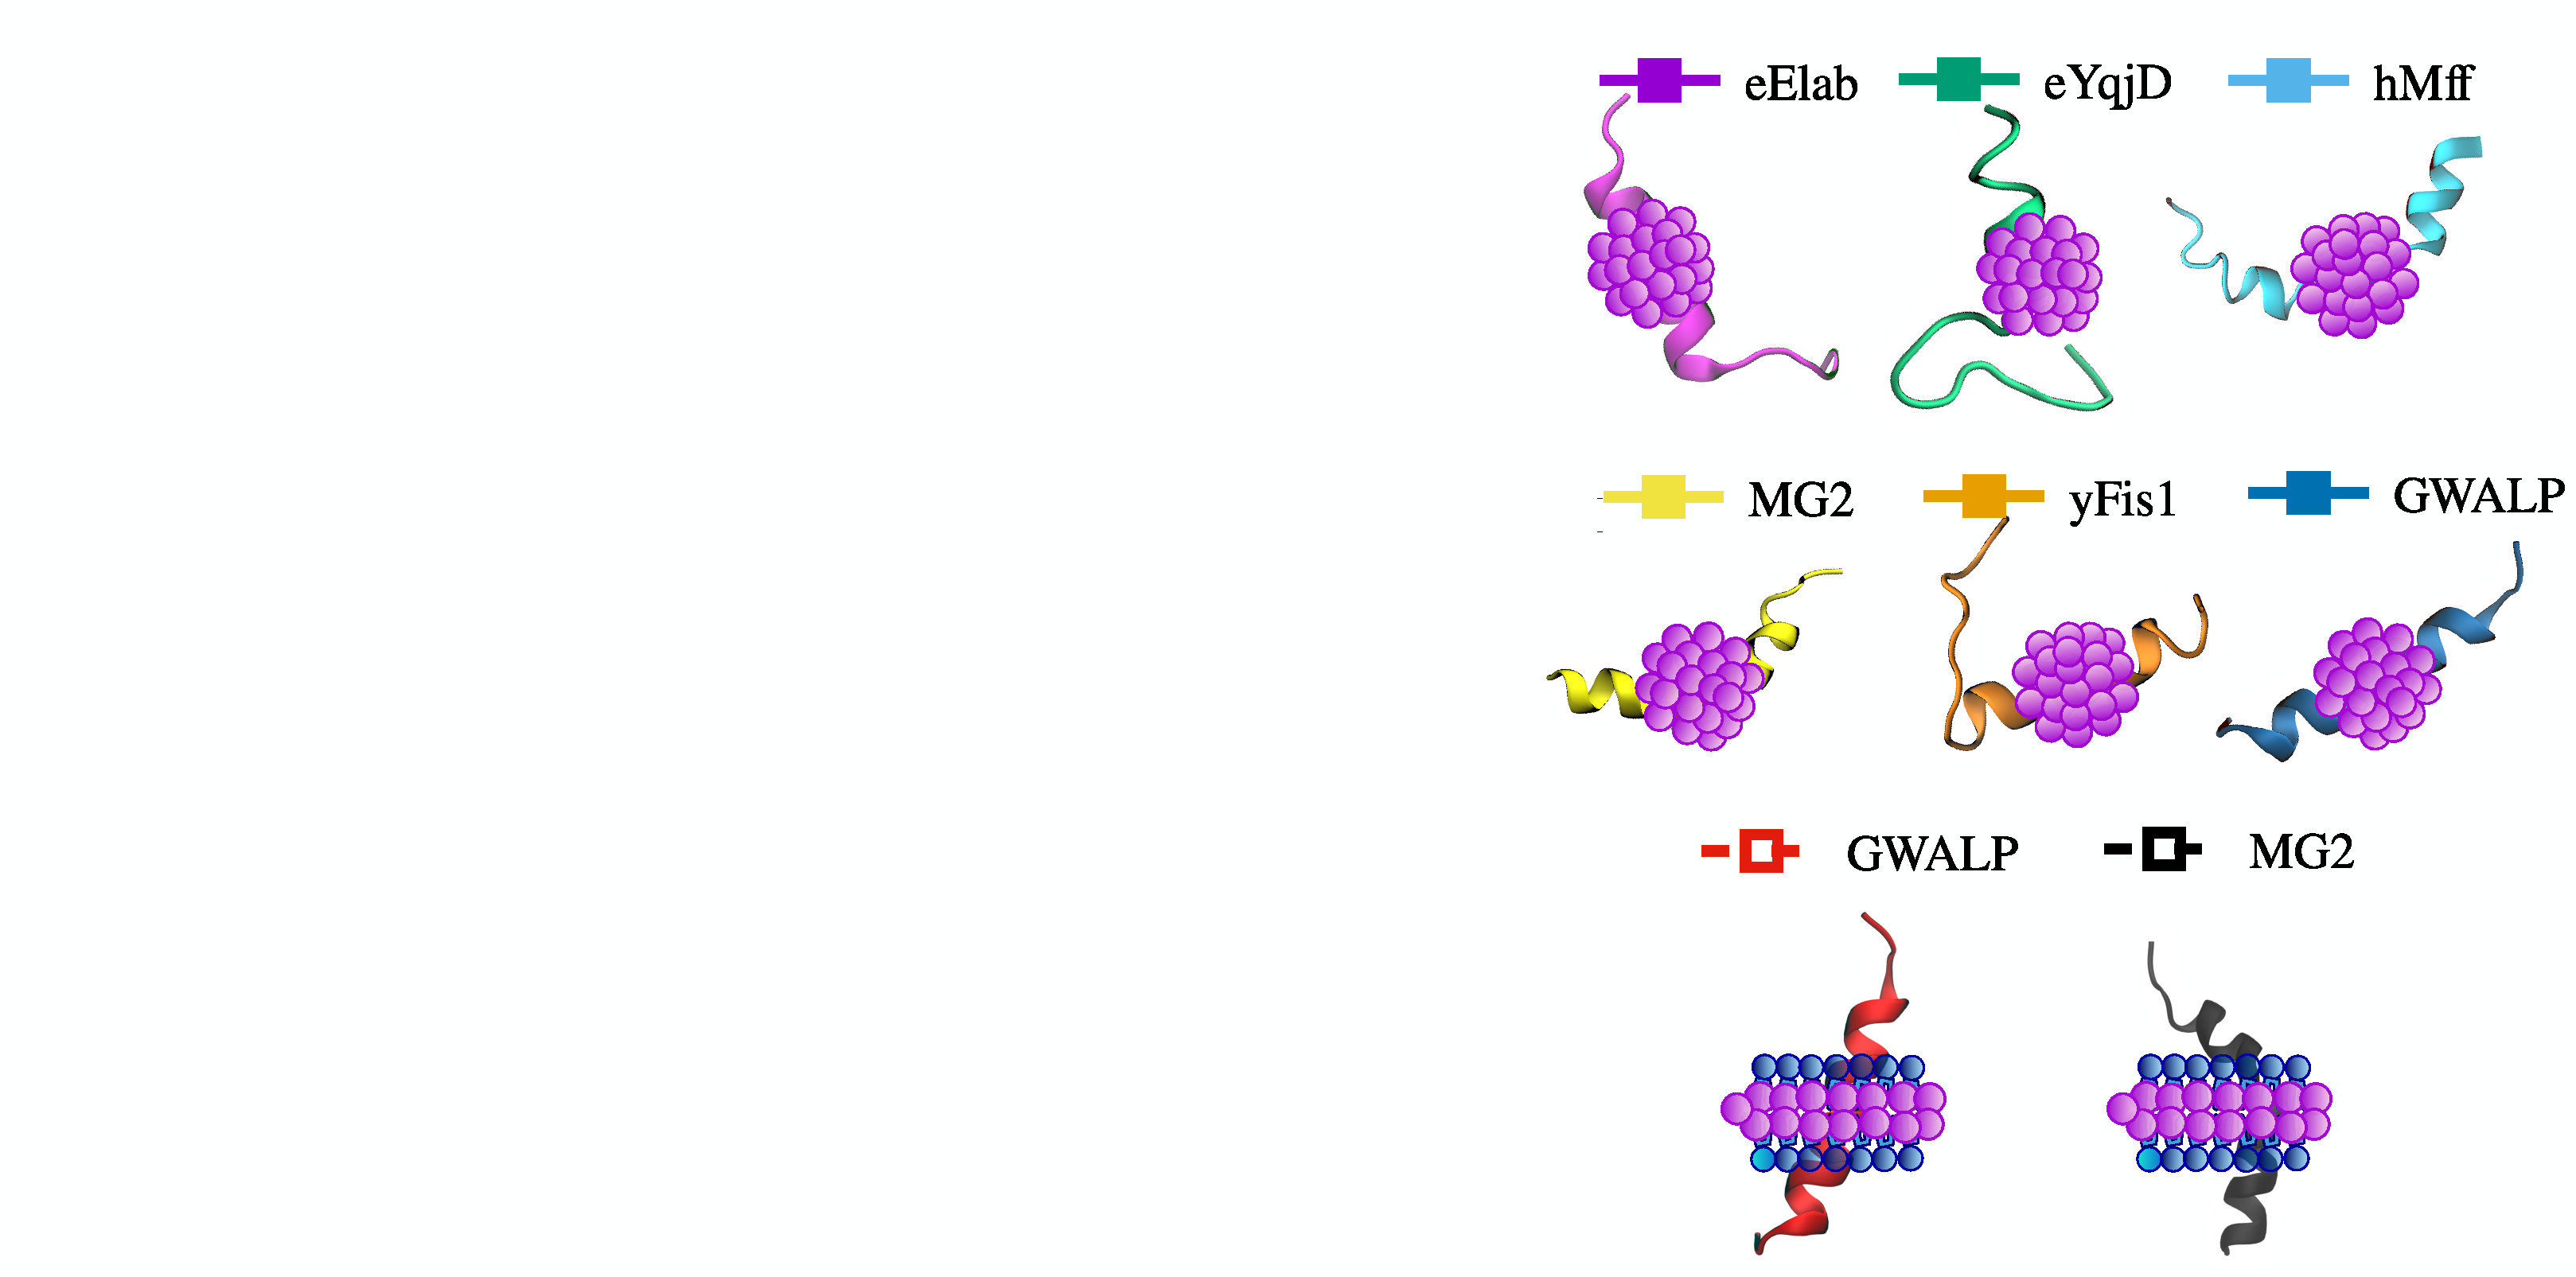
\includegraphics[height=5cm]{can_we2.pdf}
\end{center}
\end{frame}


\addtocounter{framenumber}{-1}
\begin{frame}
\begin{center}
\Large{\centering
\textbf{Goal: What can we tell about membrane proteins based on differences in spin relaxation times?} \\}

\vspace{0.5cm}

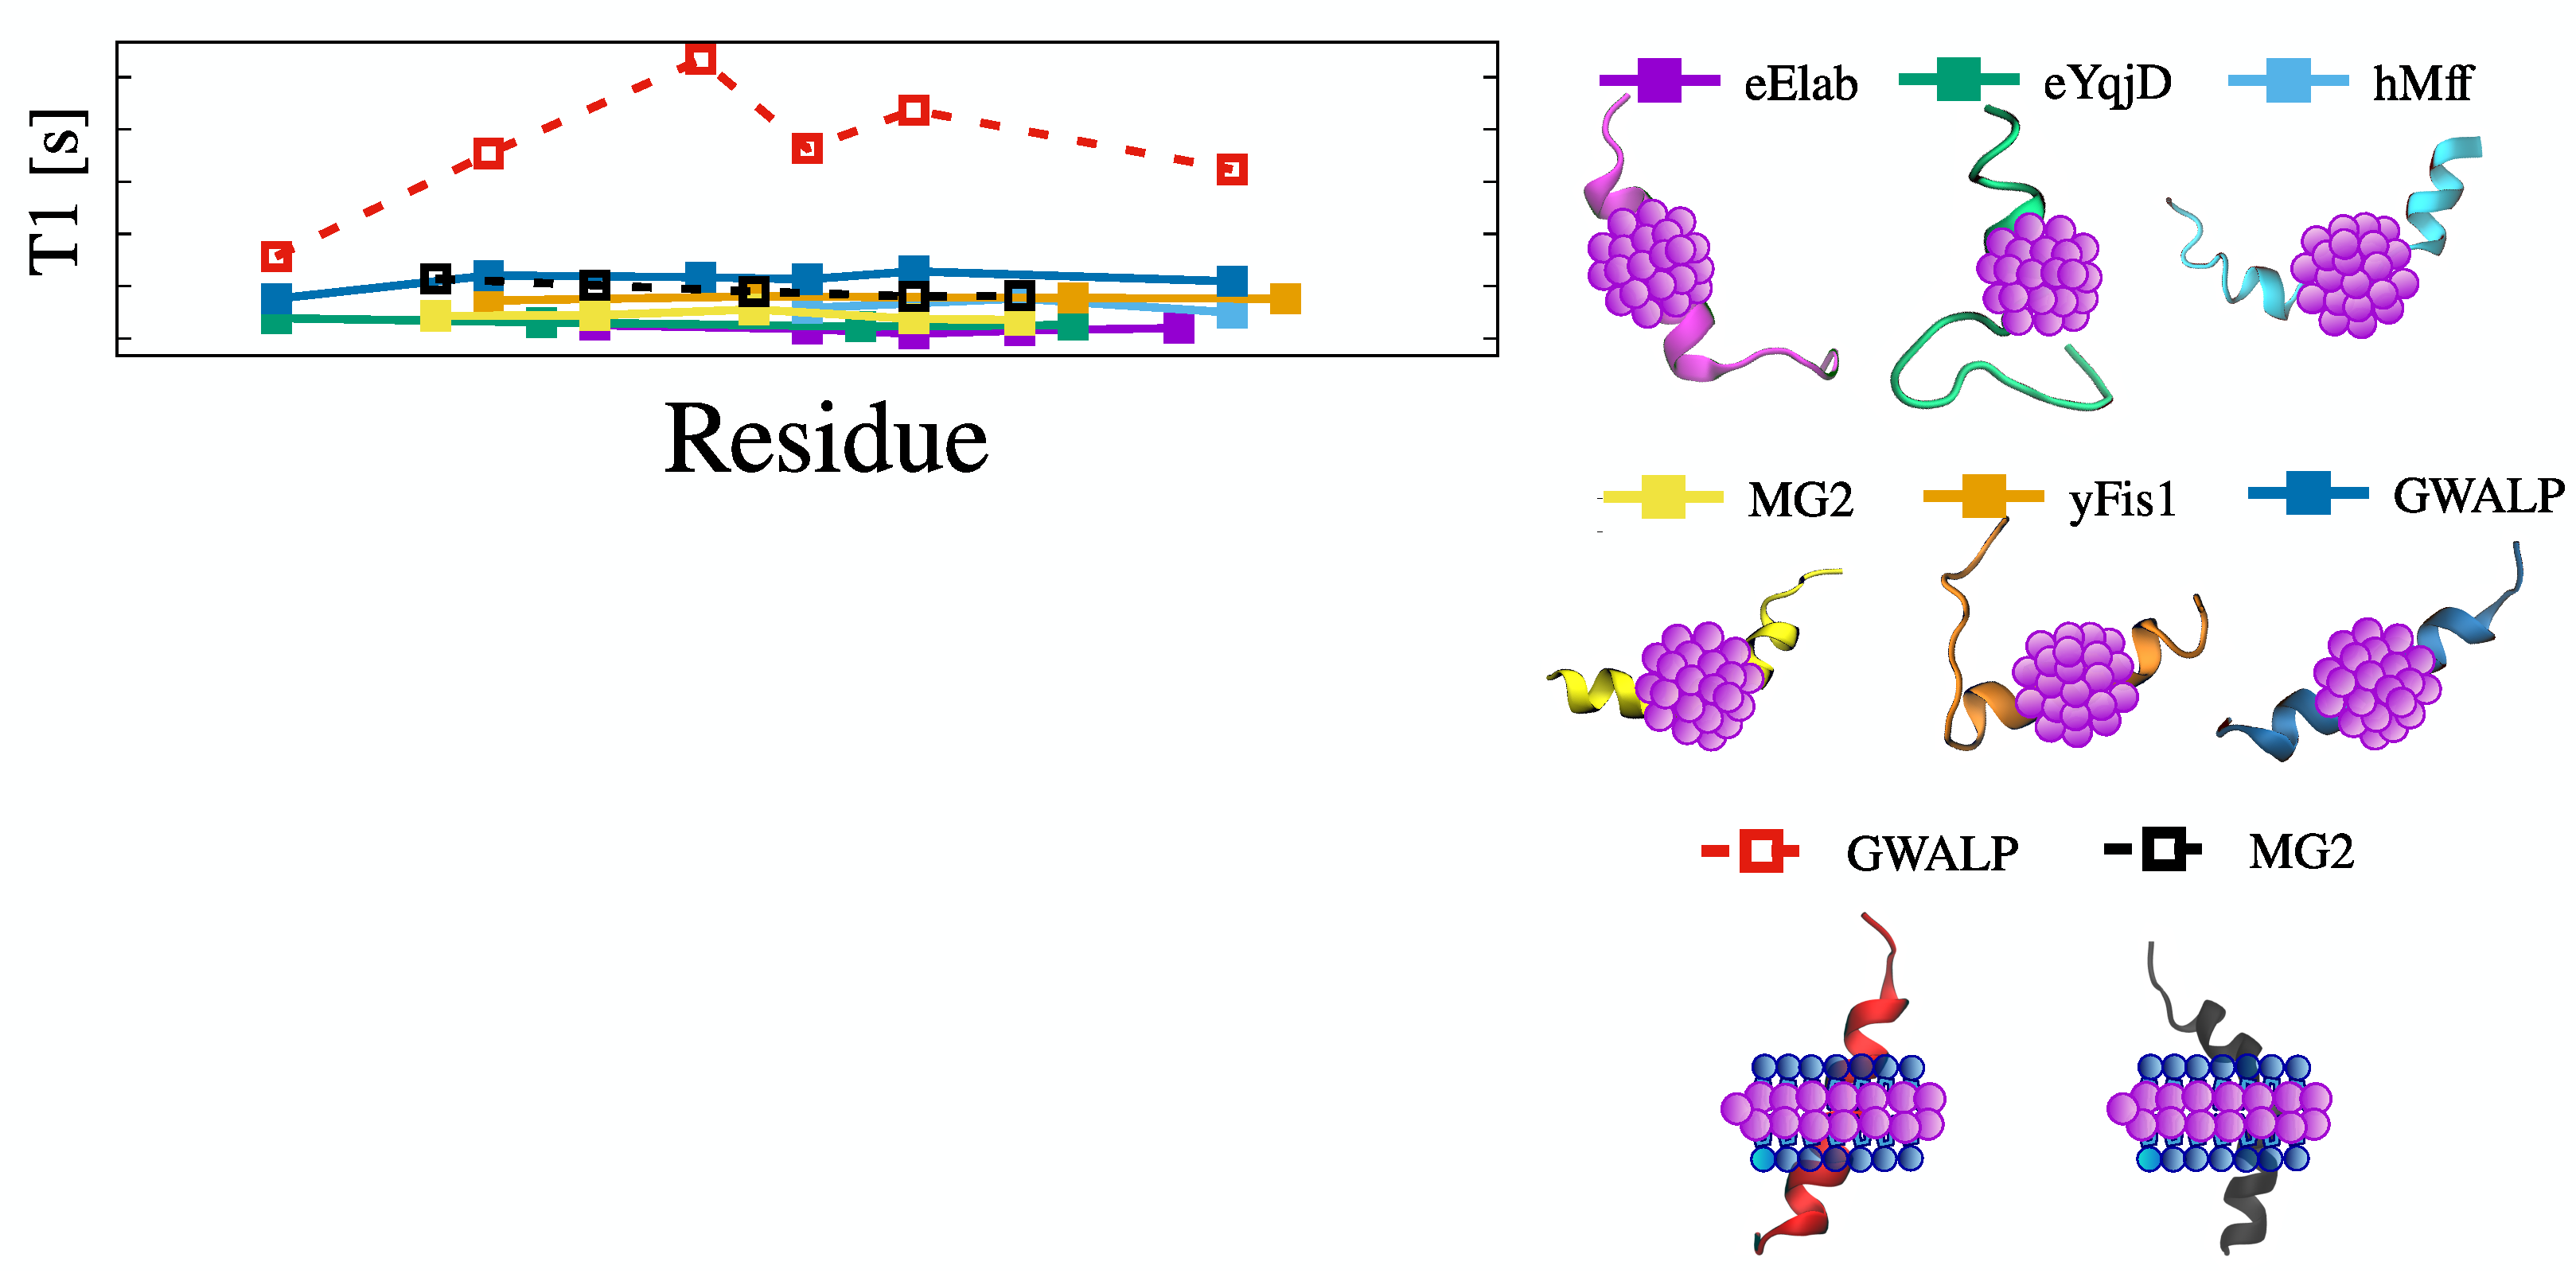
\includegraphics[height=5cm]{can_we3.pdf}
\end{center}
\end{frame}

\addtocounter{framenumber}{-1}
\begin{frame}
\begin{center}
\Large{\centering
\textbf{Goal: What can we tell about membrane proteins based on differences in spin relaxation times?} \\}

\vspace{0.5cm}

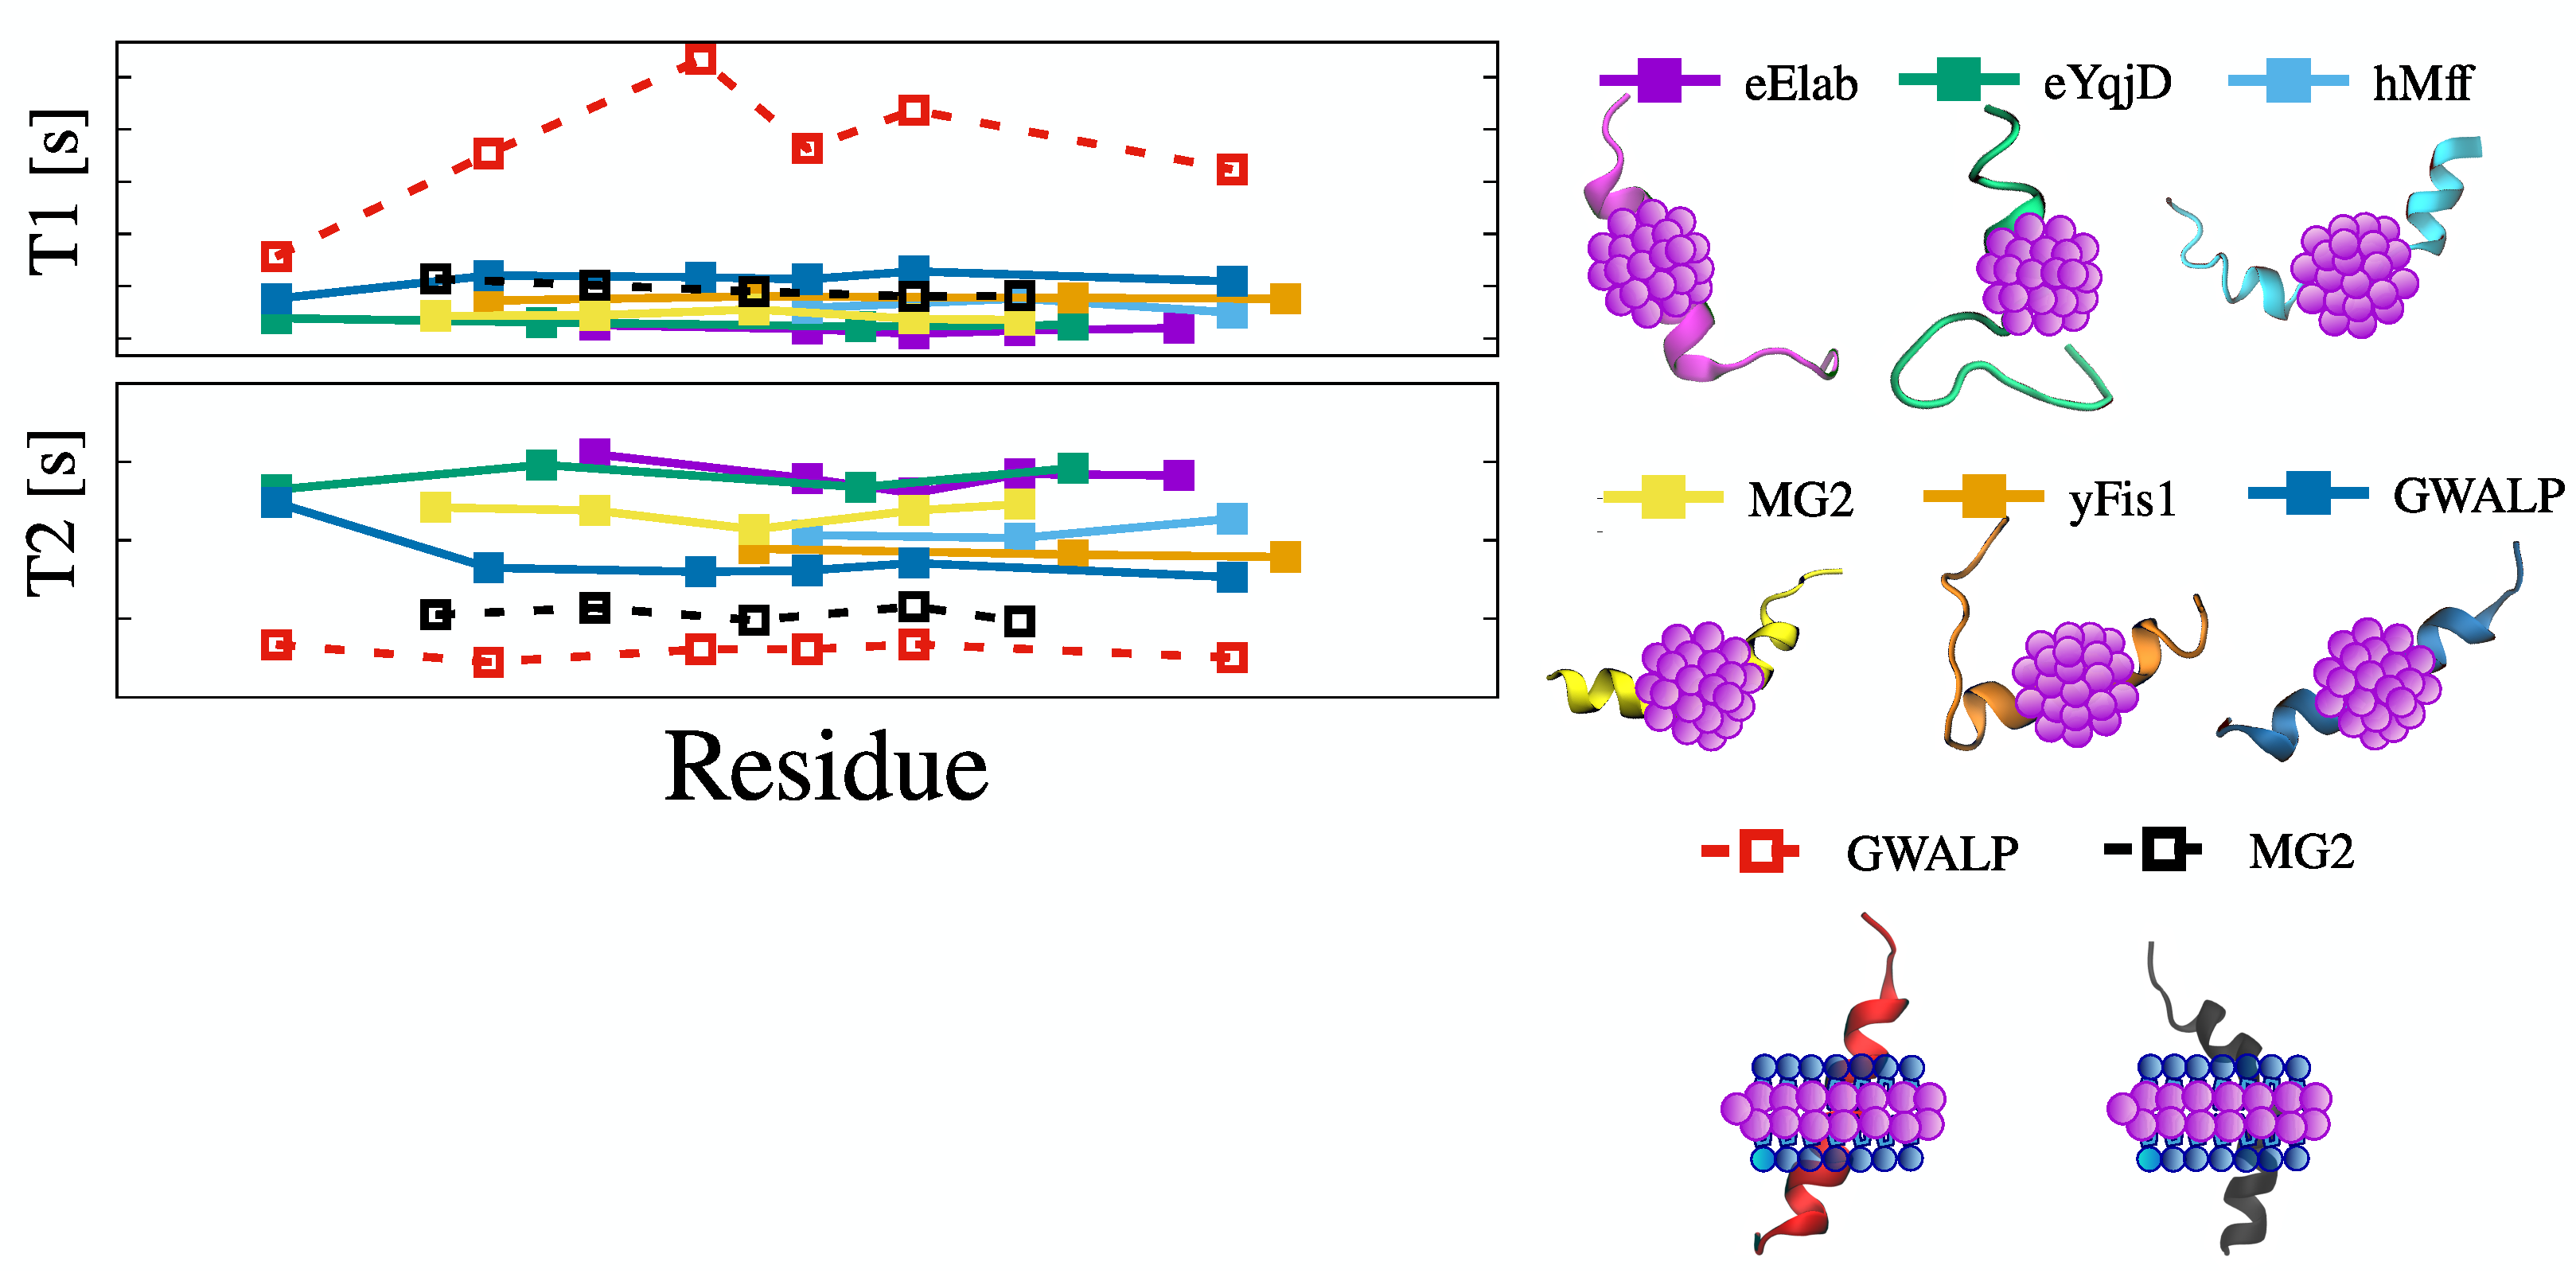
\includegraphics[height=5cm]{can_we4.pdf}
\end{center}
\end{frame}




\addtocounter{framenumber}{-1}
\begin{frame}
\begin{center}
\Large{\centering
\textbf{Goal: What can we tell about membrane proteins based on differences in spin relaxation times?} \\}

\vspace{0.5cm}

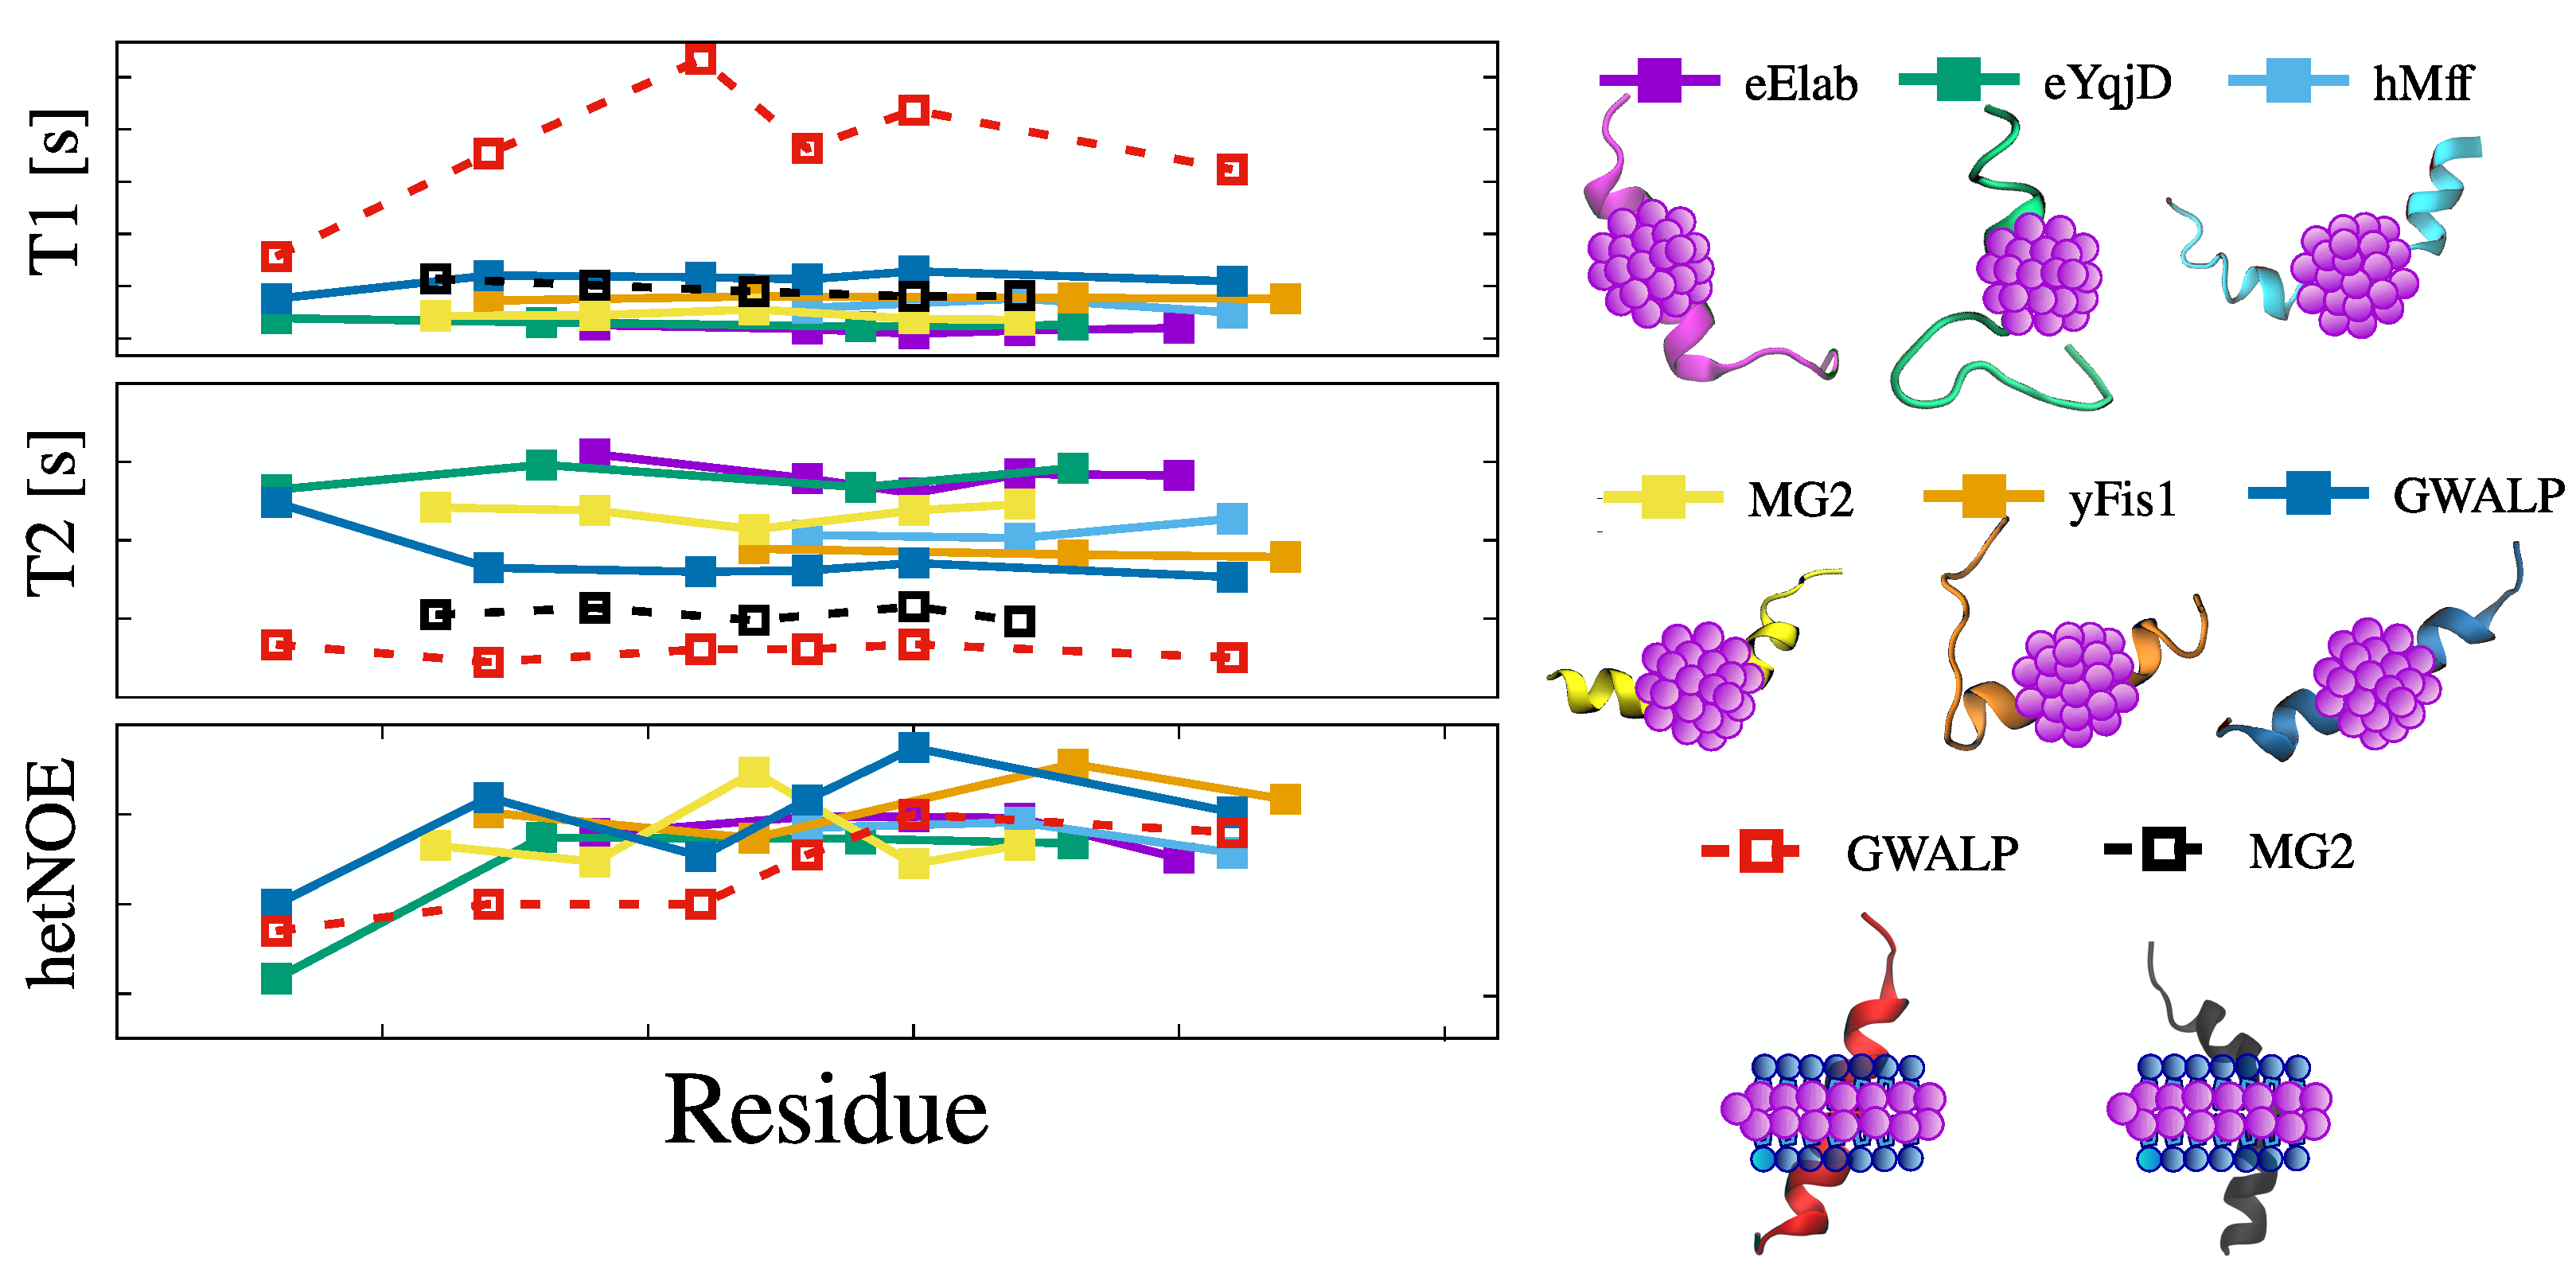
\includegraphics[height=5cm]{can_we.pdf}
\end{center}
\end{frame}



\subsection{How}

\begin{frame}
\begin{center}
\Large{\centering
\textbf{How do we actually do it?} \\}

\vspace{0.5cm}

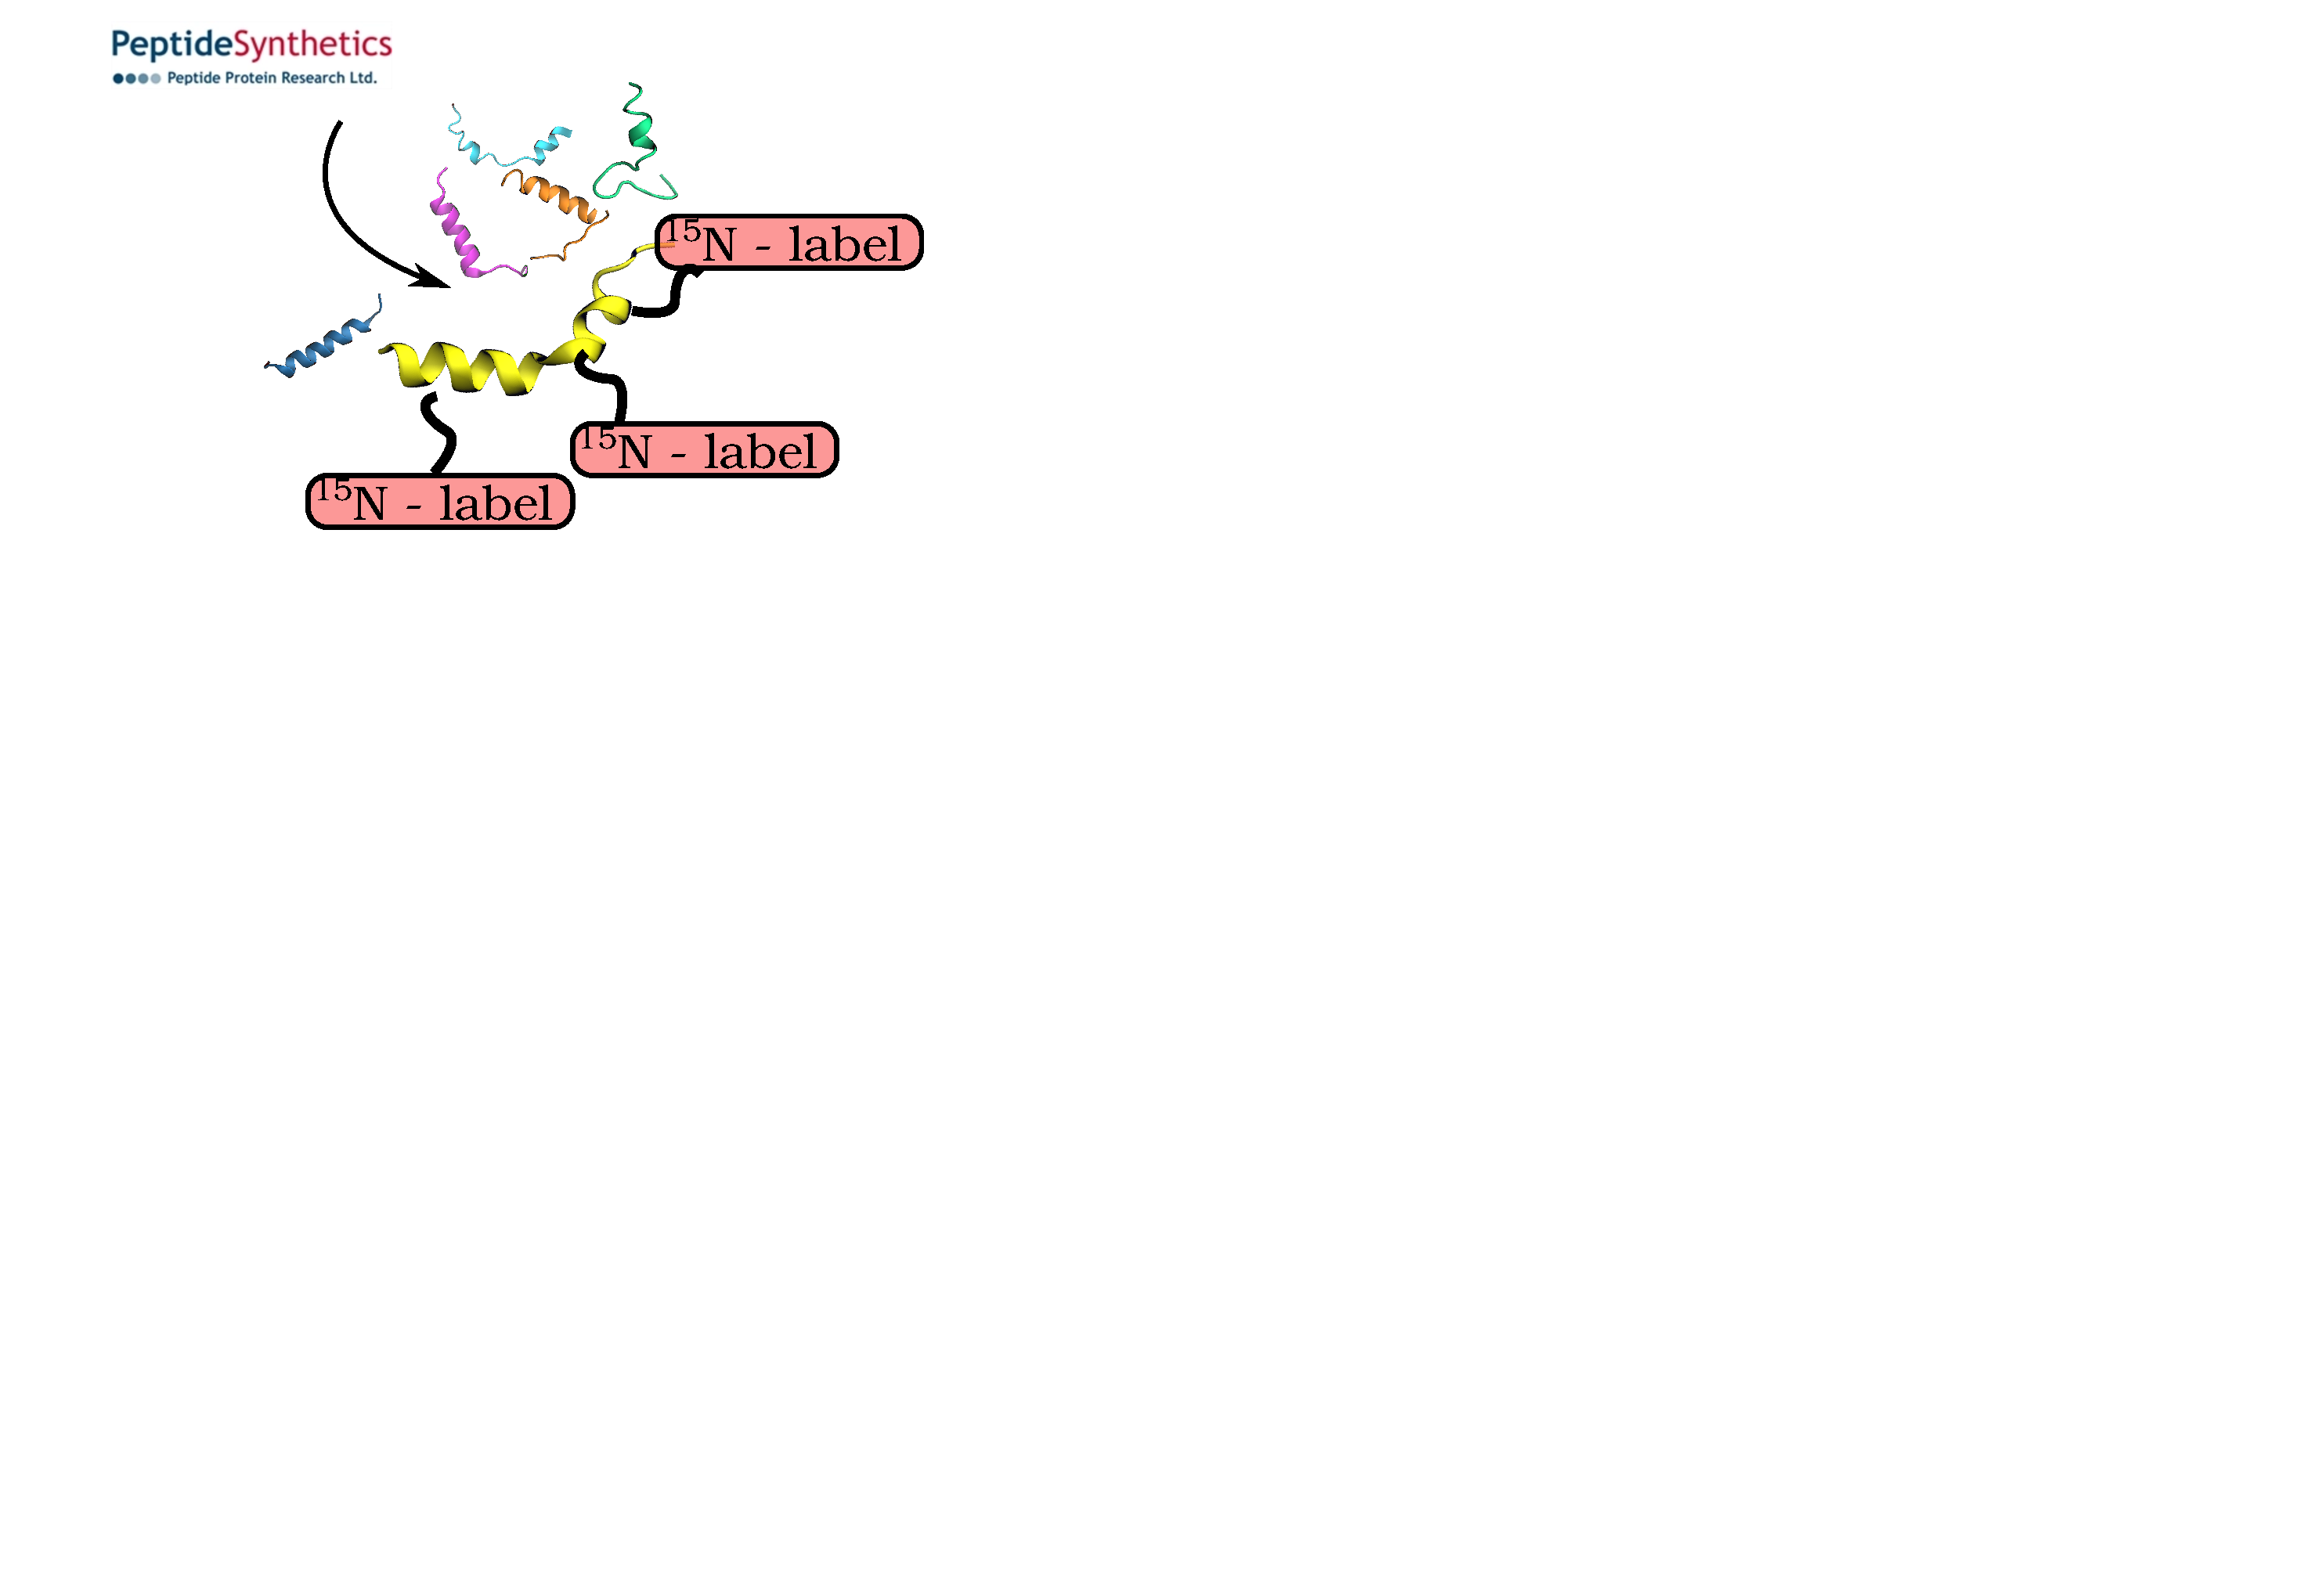
\includegraphics[height=6cm]{what_we_do11.pdf}
\end{center}
\end{frame}

\addtocounter{framenumber}{-1}
\begin{frame}
\begin{center}
\Large{\centering
\textbf{How do we actually do it?} \\}

\vspace{0.5cm}

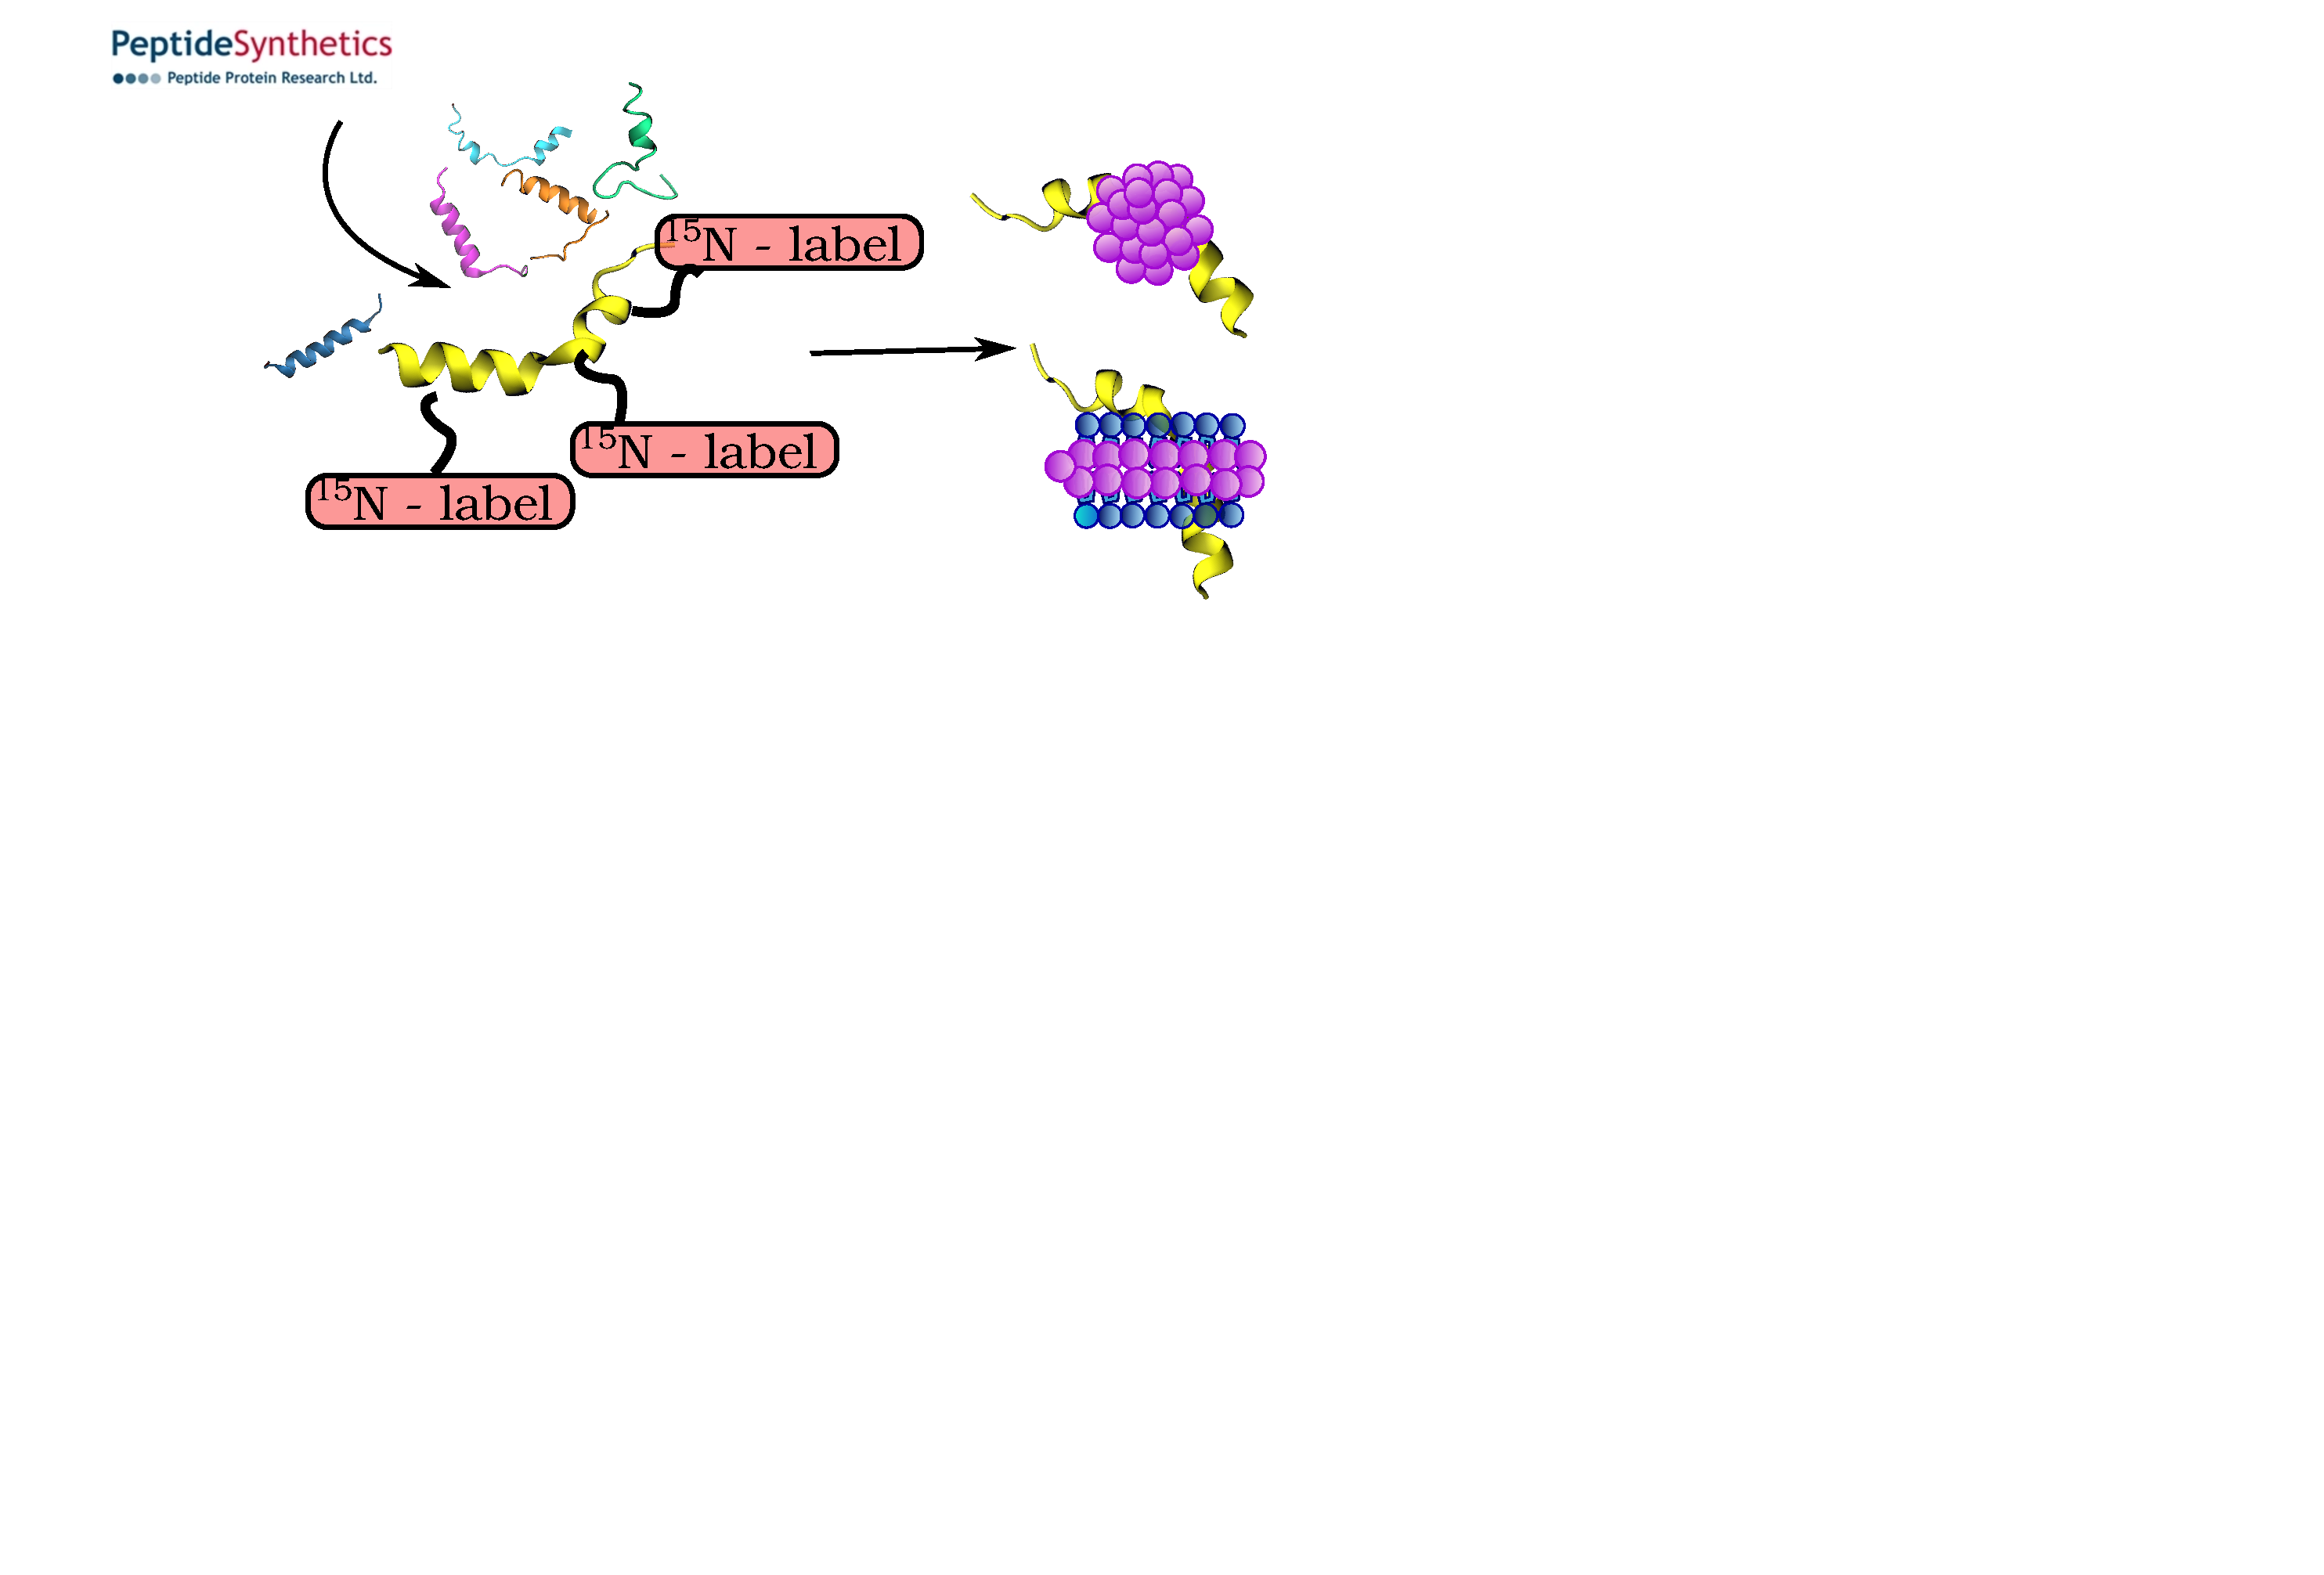
\includegraphics[height=6cm]{what_we_do10.pdf}
\end{center}
\end{frame}


\addtocounter{framenumber}{-1}
\begin{frame}
\begin{center}
\Large{\centering
\textbf{How do we actually do it?} \\}

\vspace{0.5cm}

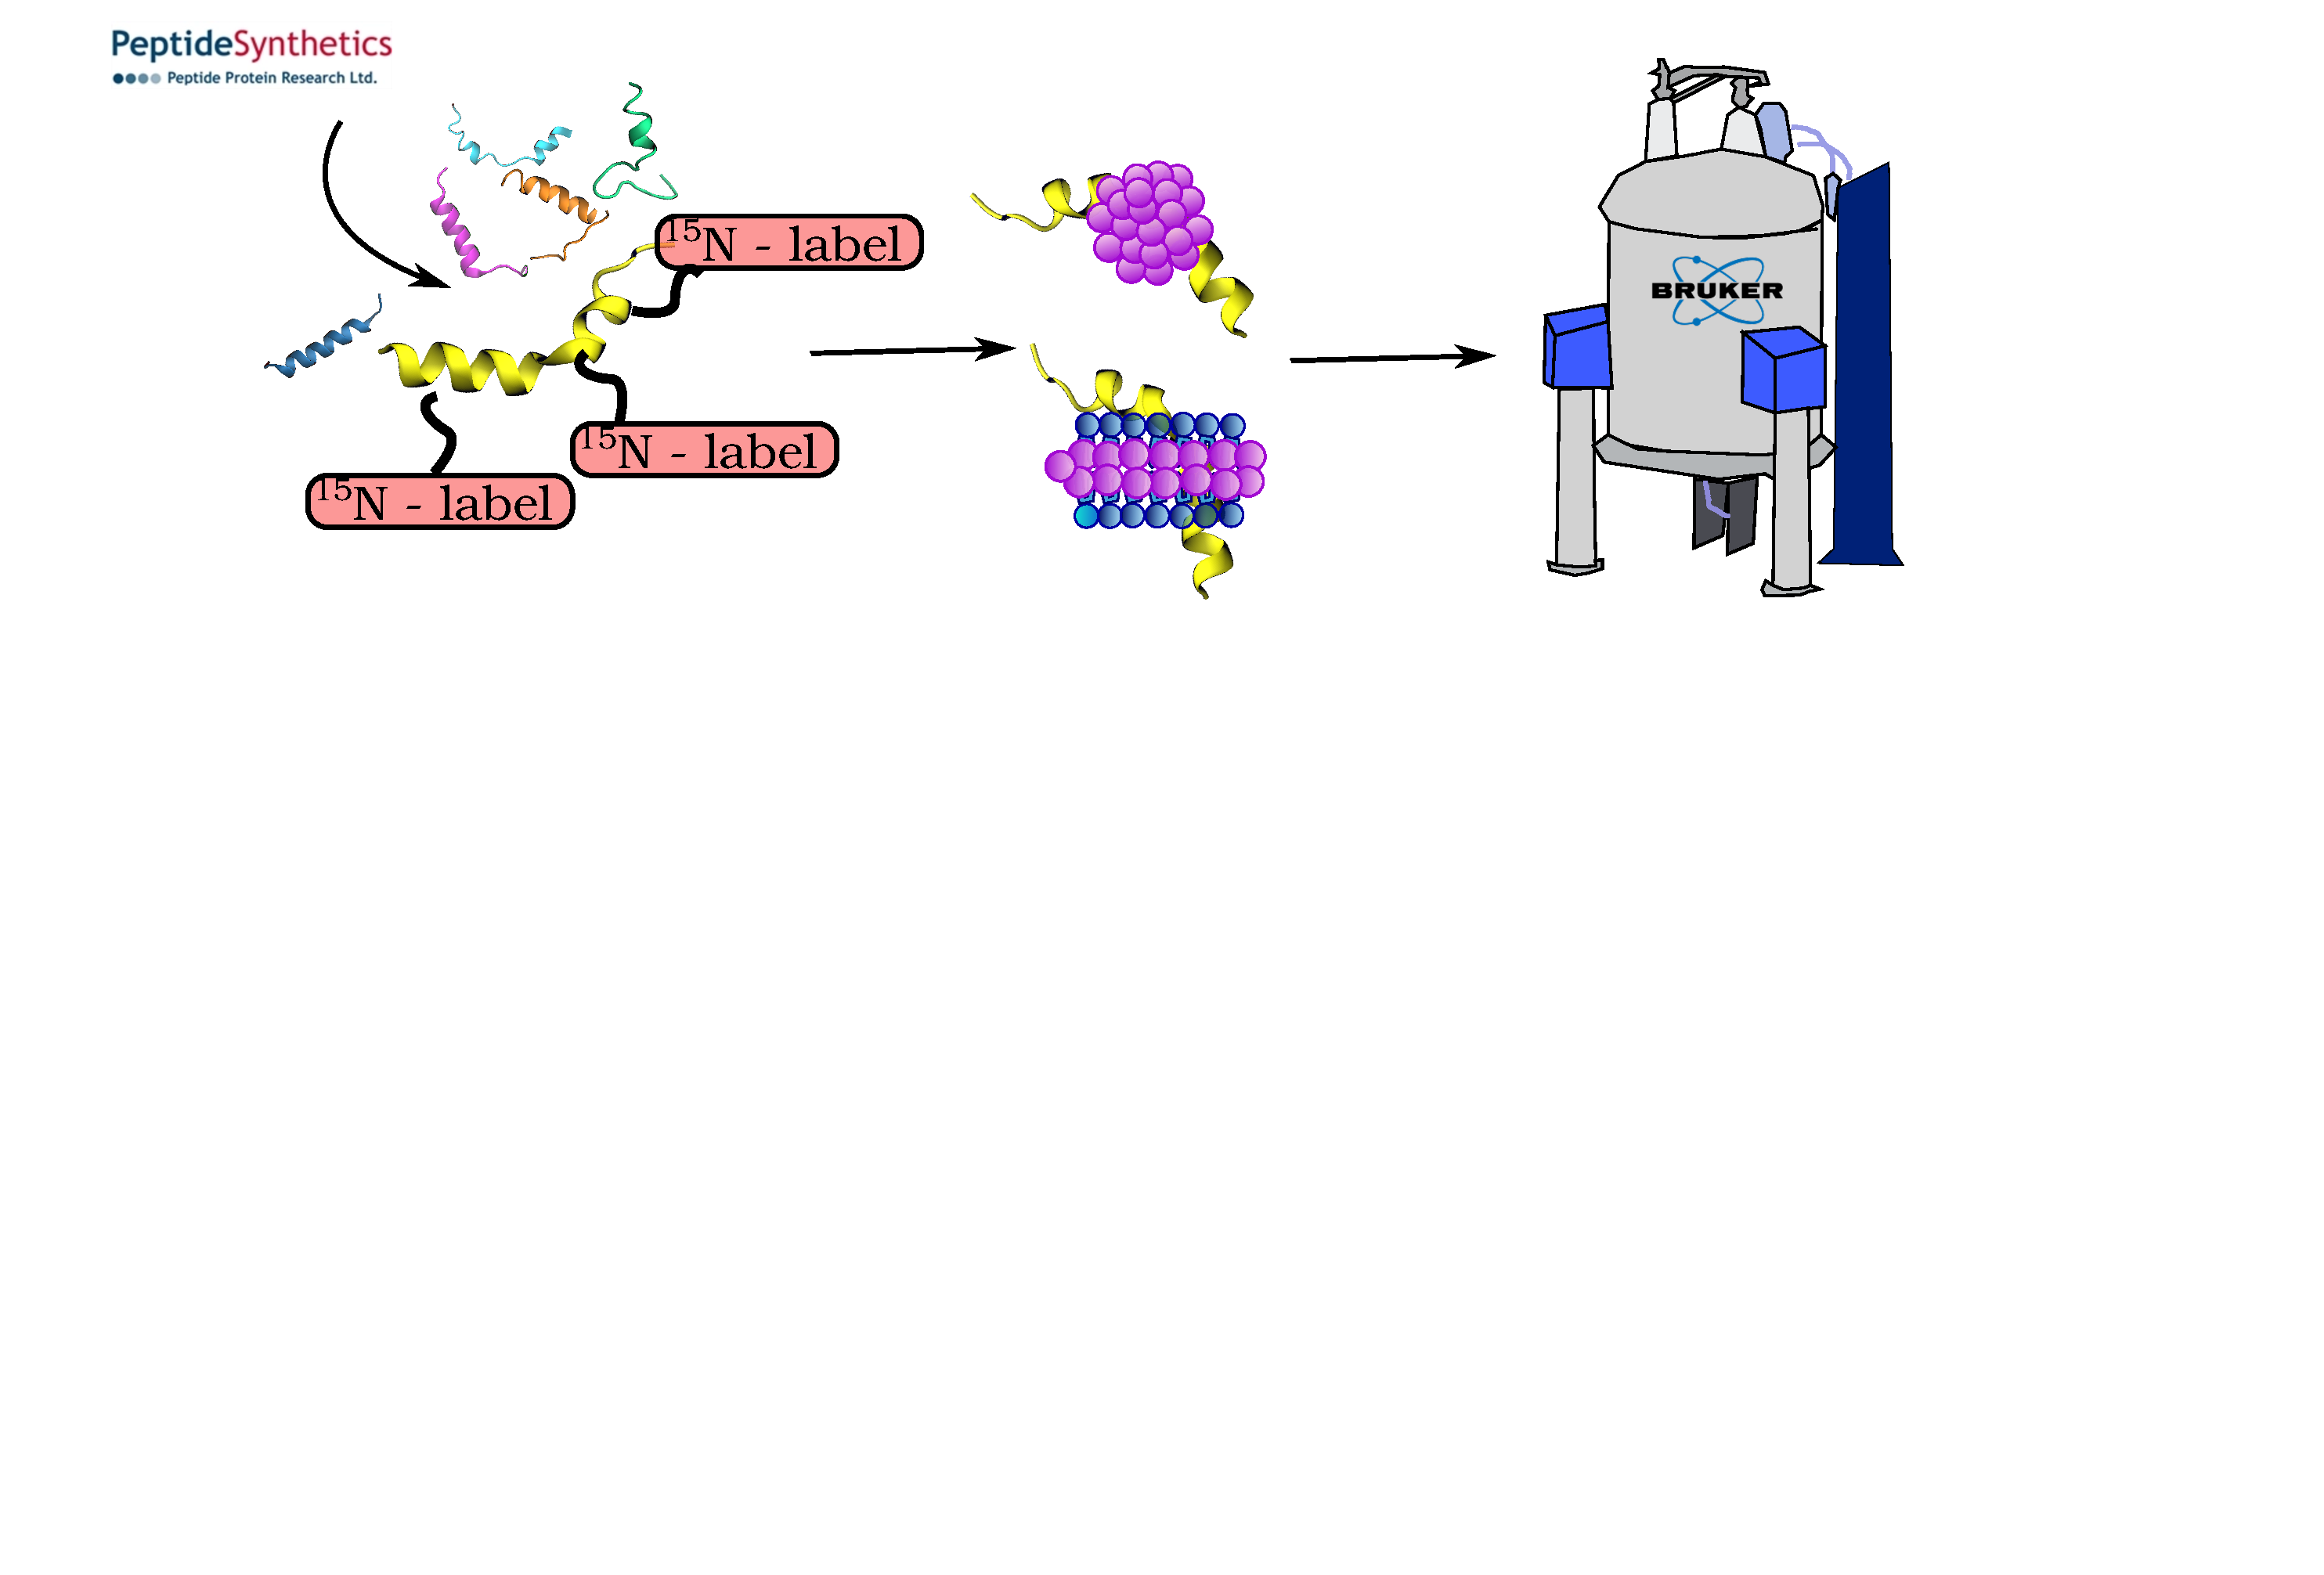
\includegraphics[height=6cm]{what_we_do9.pdf}
\end{center}
\end{frame}


\addtocounter{framenumber}{-1}
\begin{frame}
\begin{center}
\Large{\centering
\textbf{How do we actually do it?} \\}

\vspace{0.5cm}

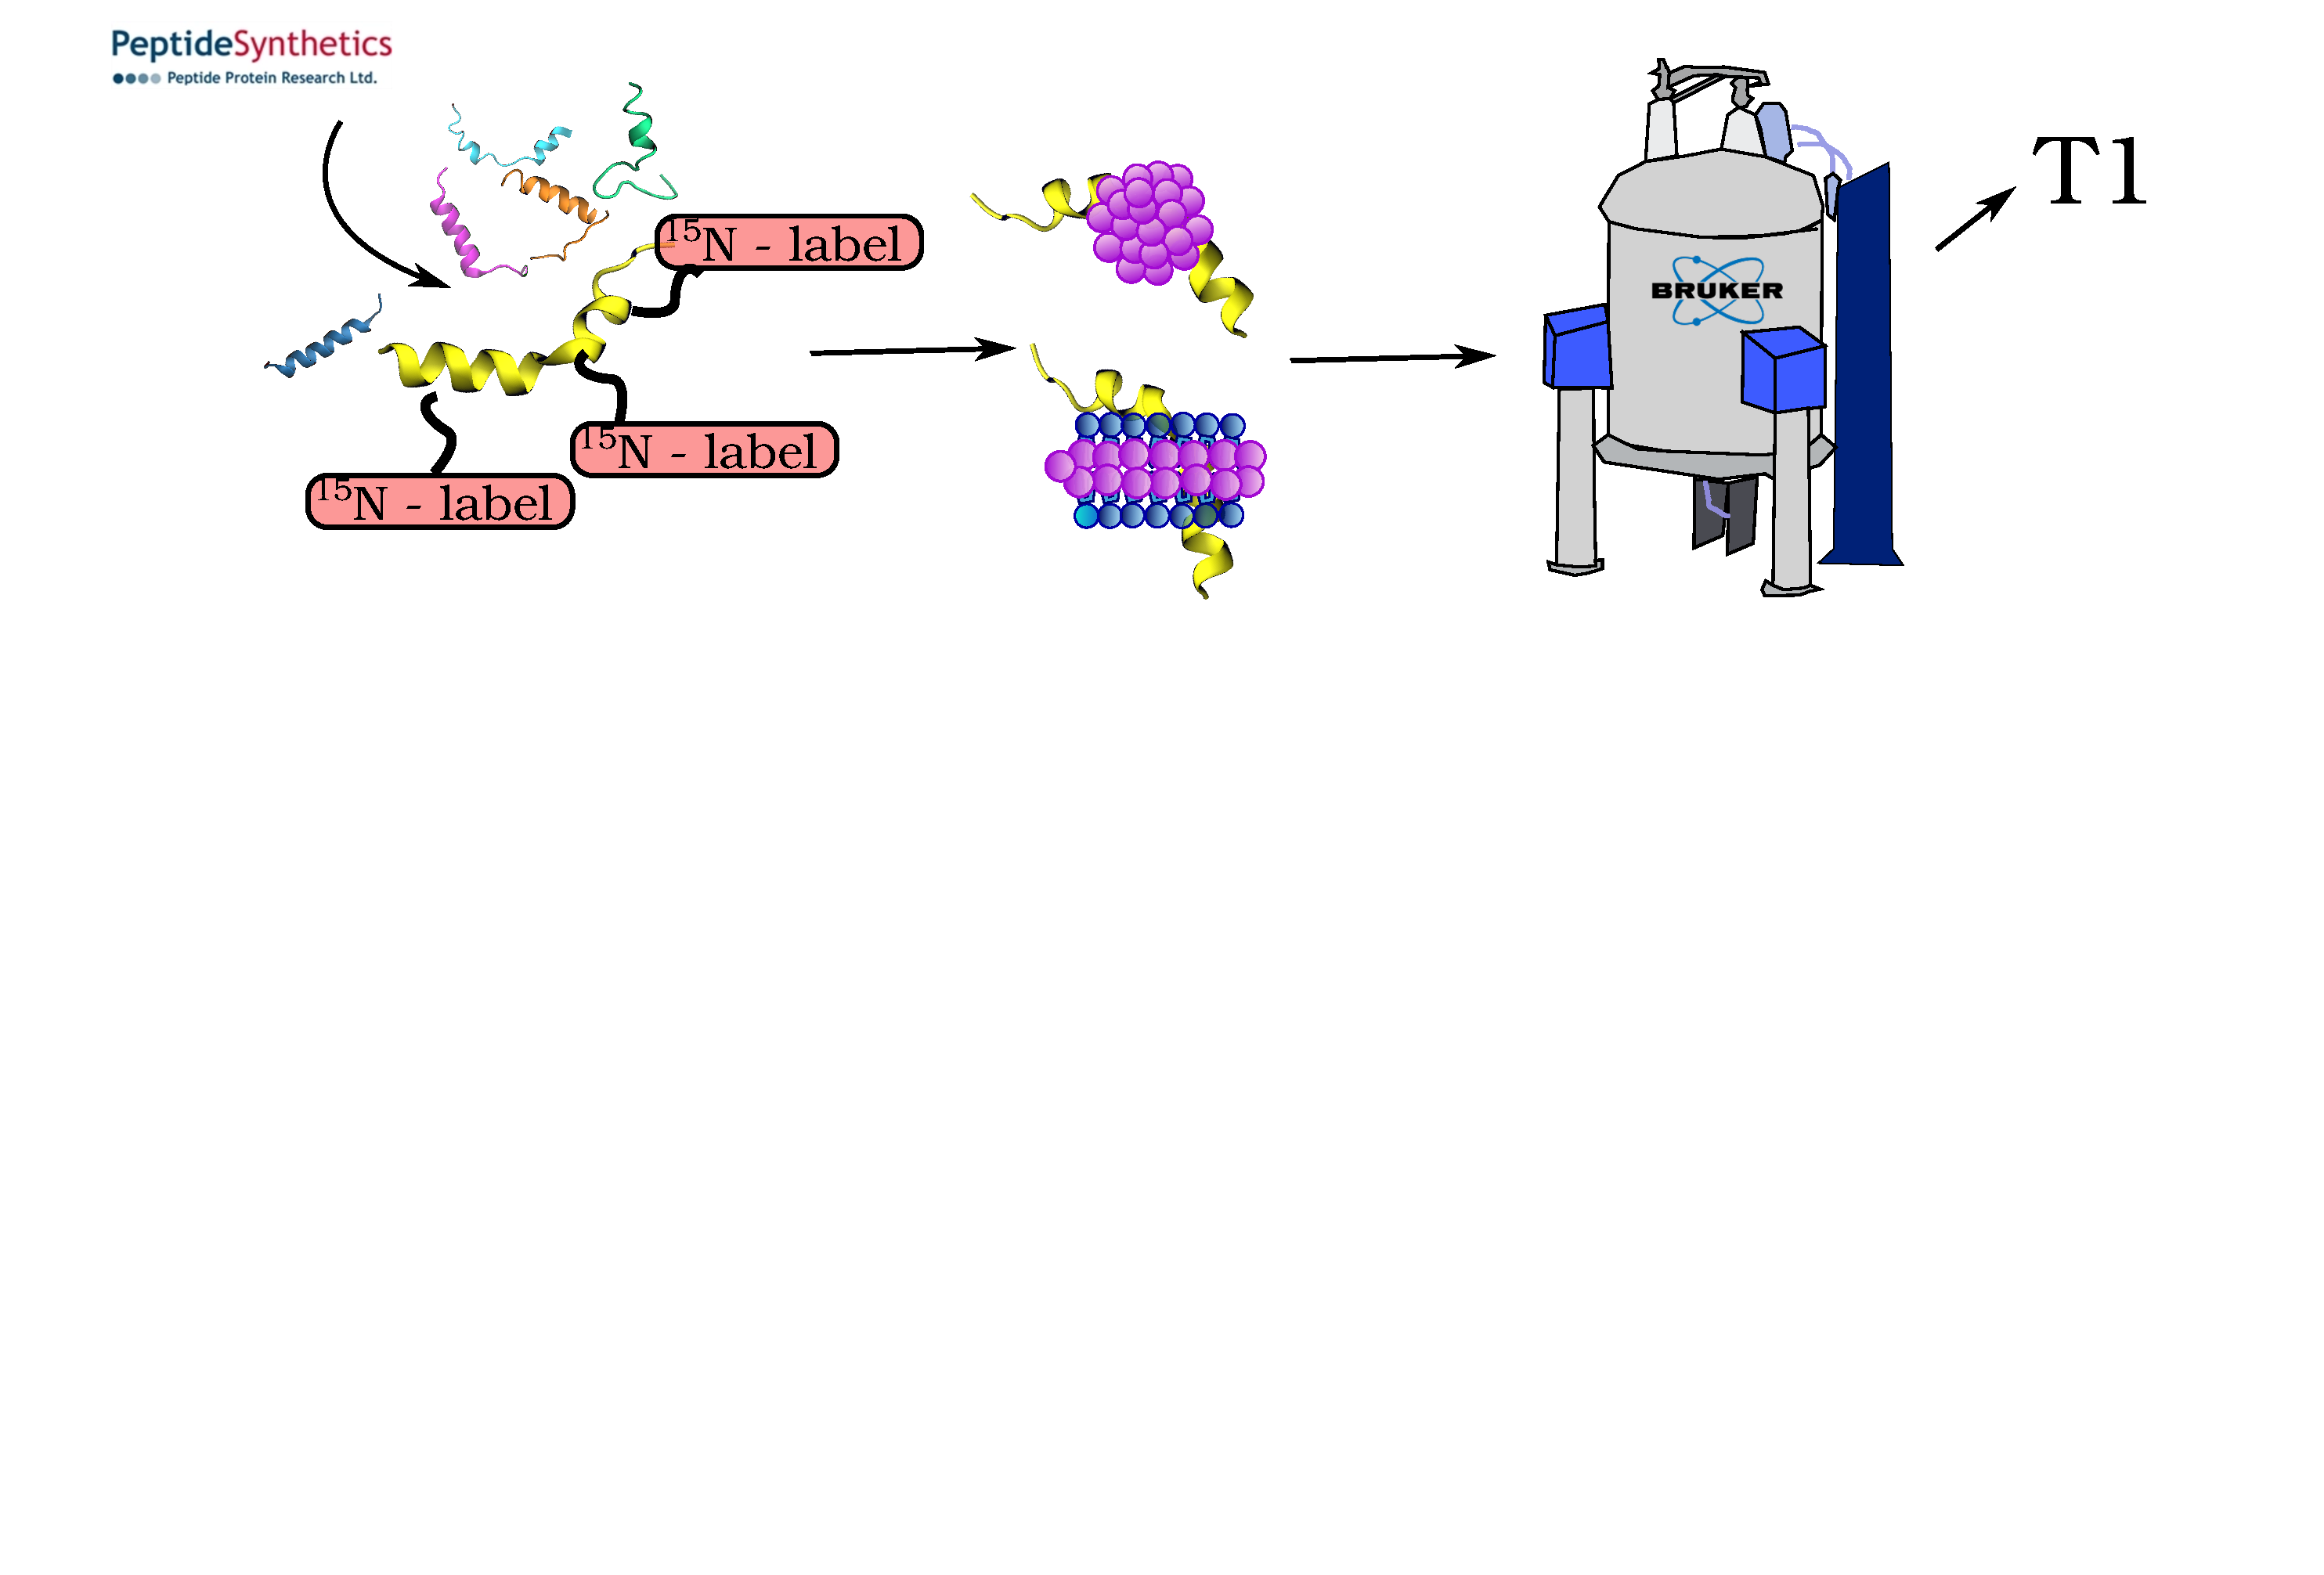
\includegraphics[height=6cm]{what_we_do8.pdf}
\end{center}
\end{frame}



\addtocounter{framenumber}{-1}
\begin{frame}
\begin{center}
\Large{\centering
\textbf{How do we actually do it?} \\}

\vspace{0.5cm}

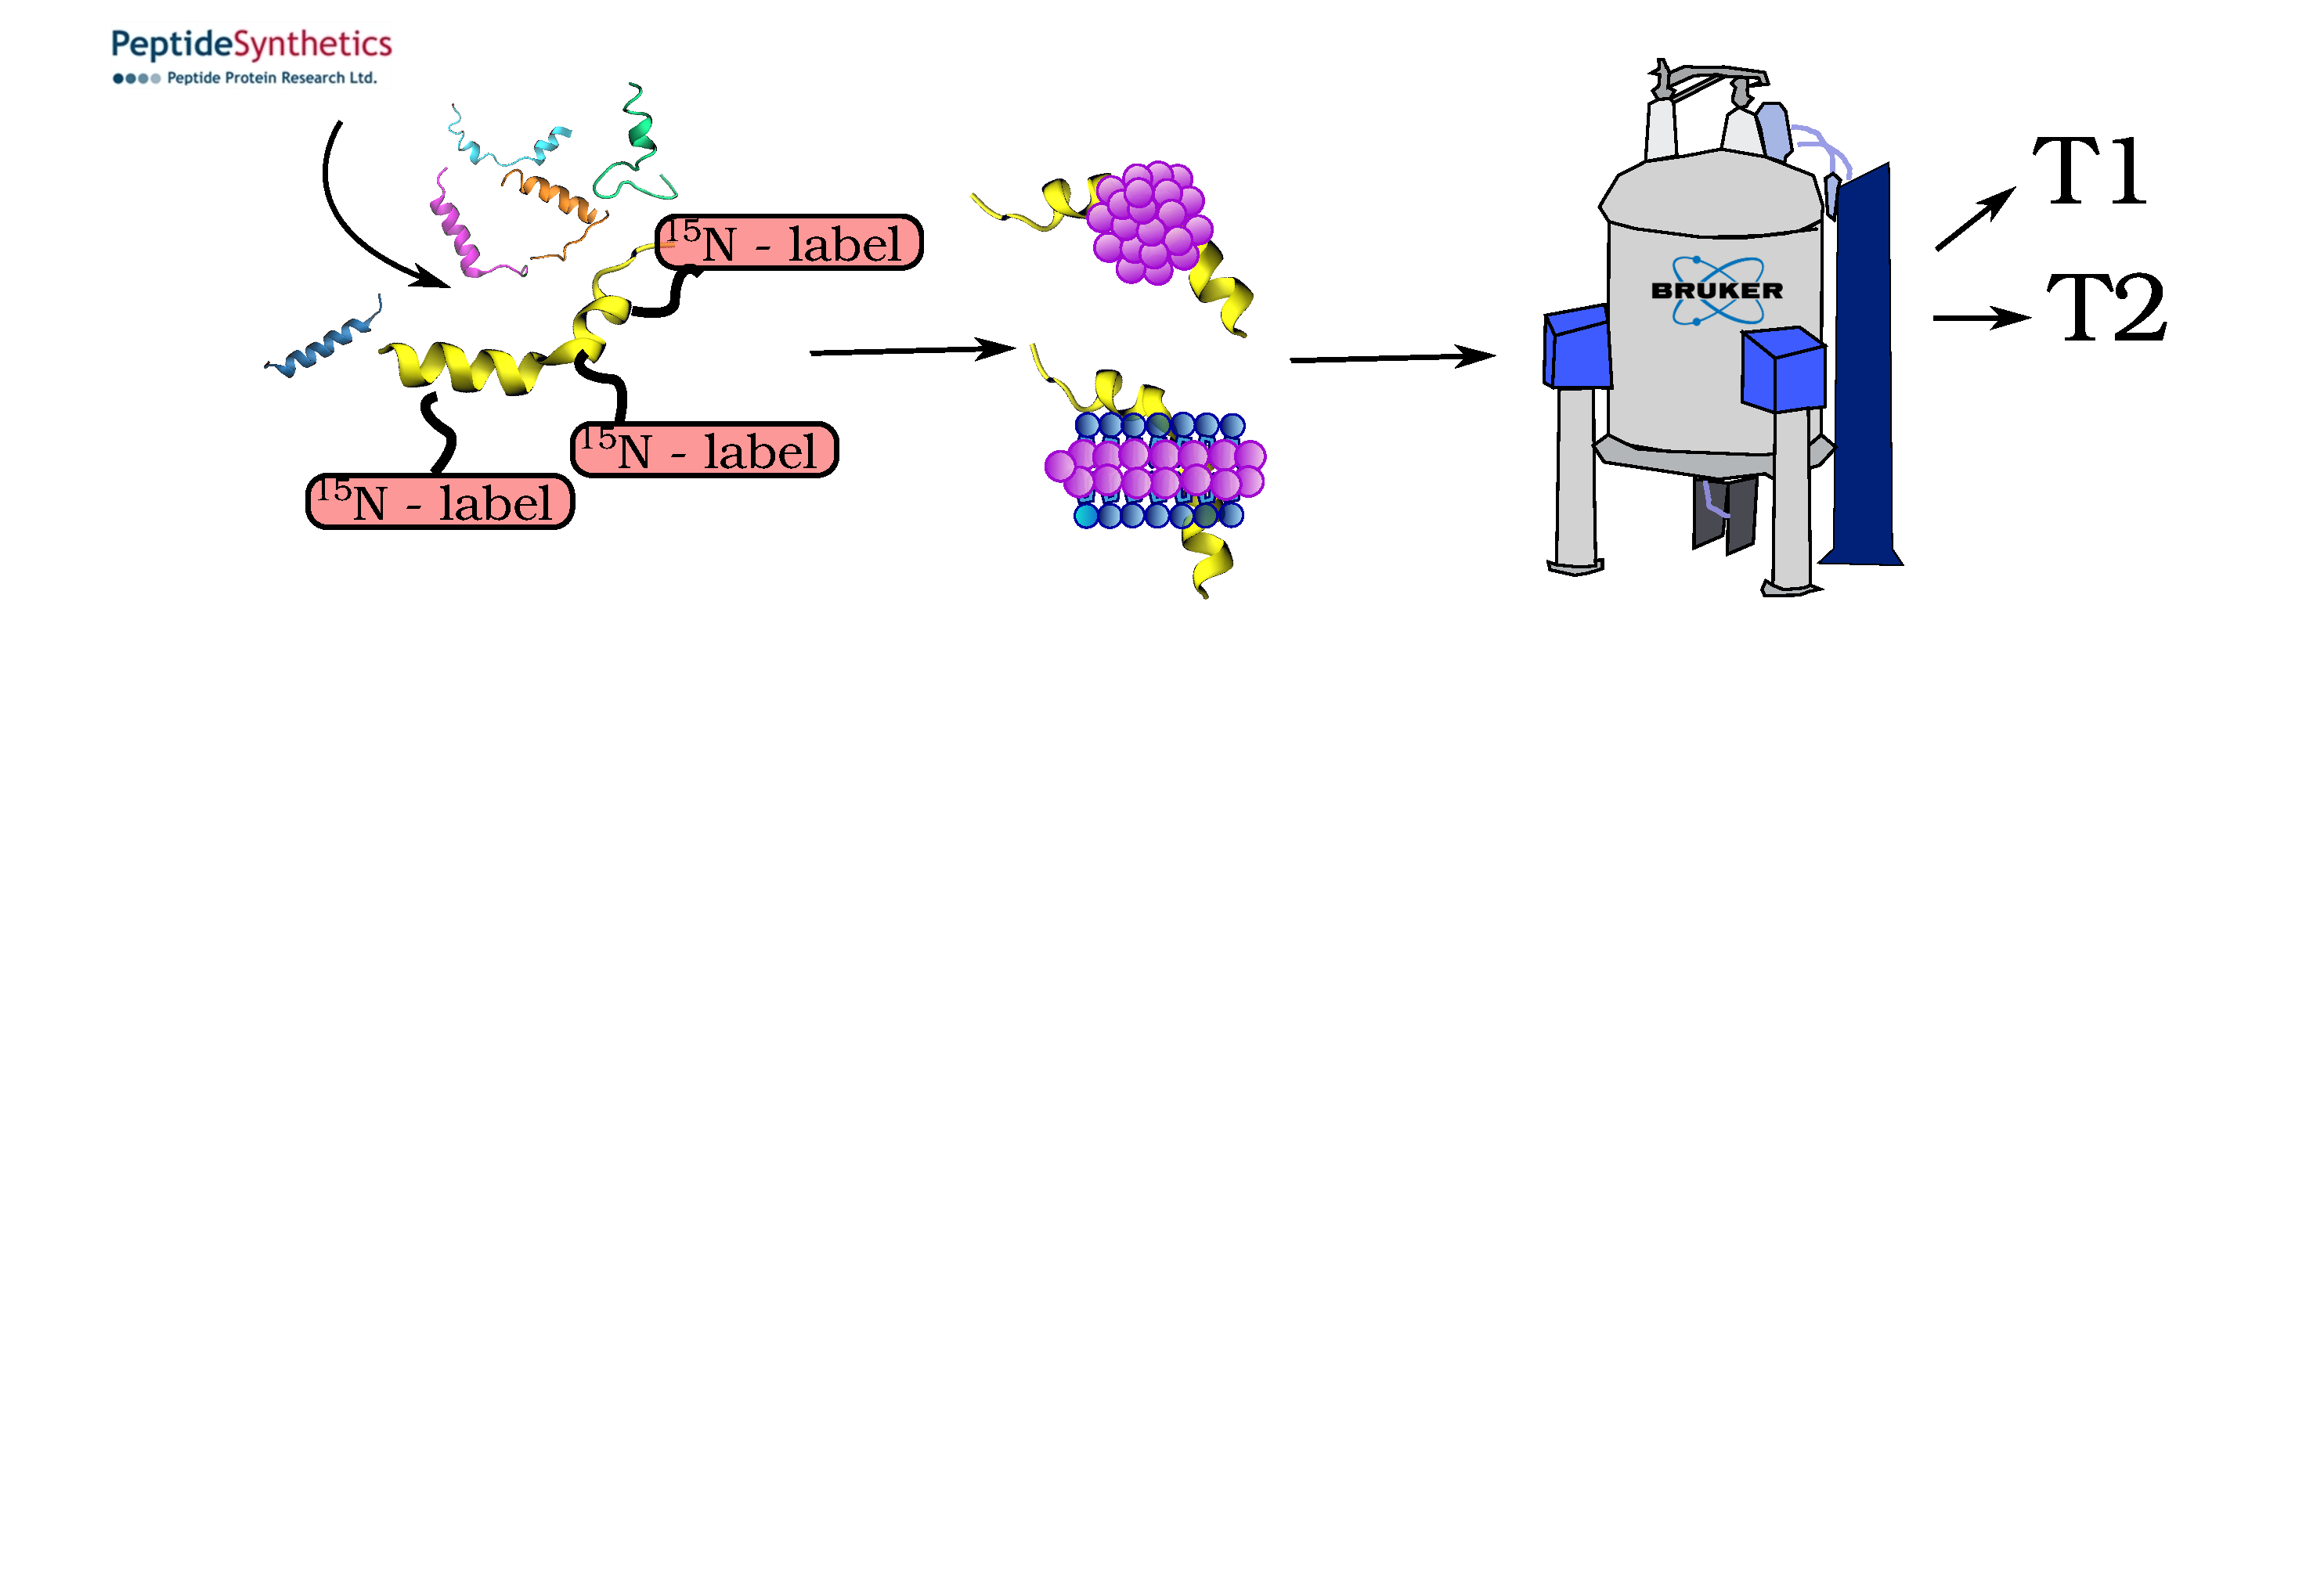
\includegraphics[height=6cm]{what_we_do7.pdf}
\end{center}
\end{frame}


\addtocounter{framenumber}{-1}
\begin{frame}
\begin{center}
\Large{\centering
\textbf{How do we actually do it?} \\}

\vspace{0.5cm}

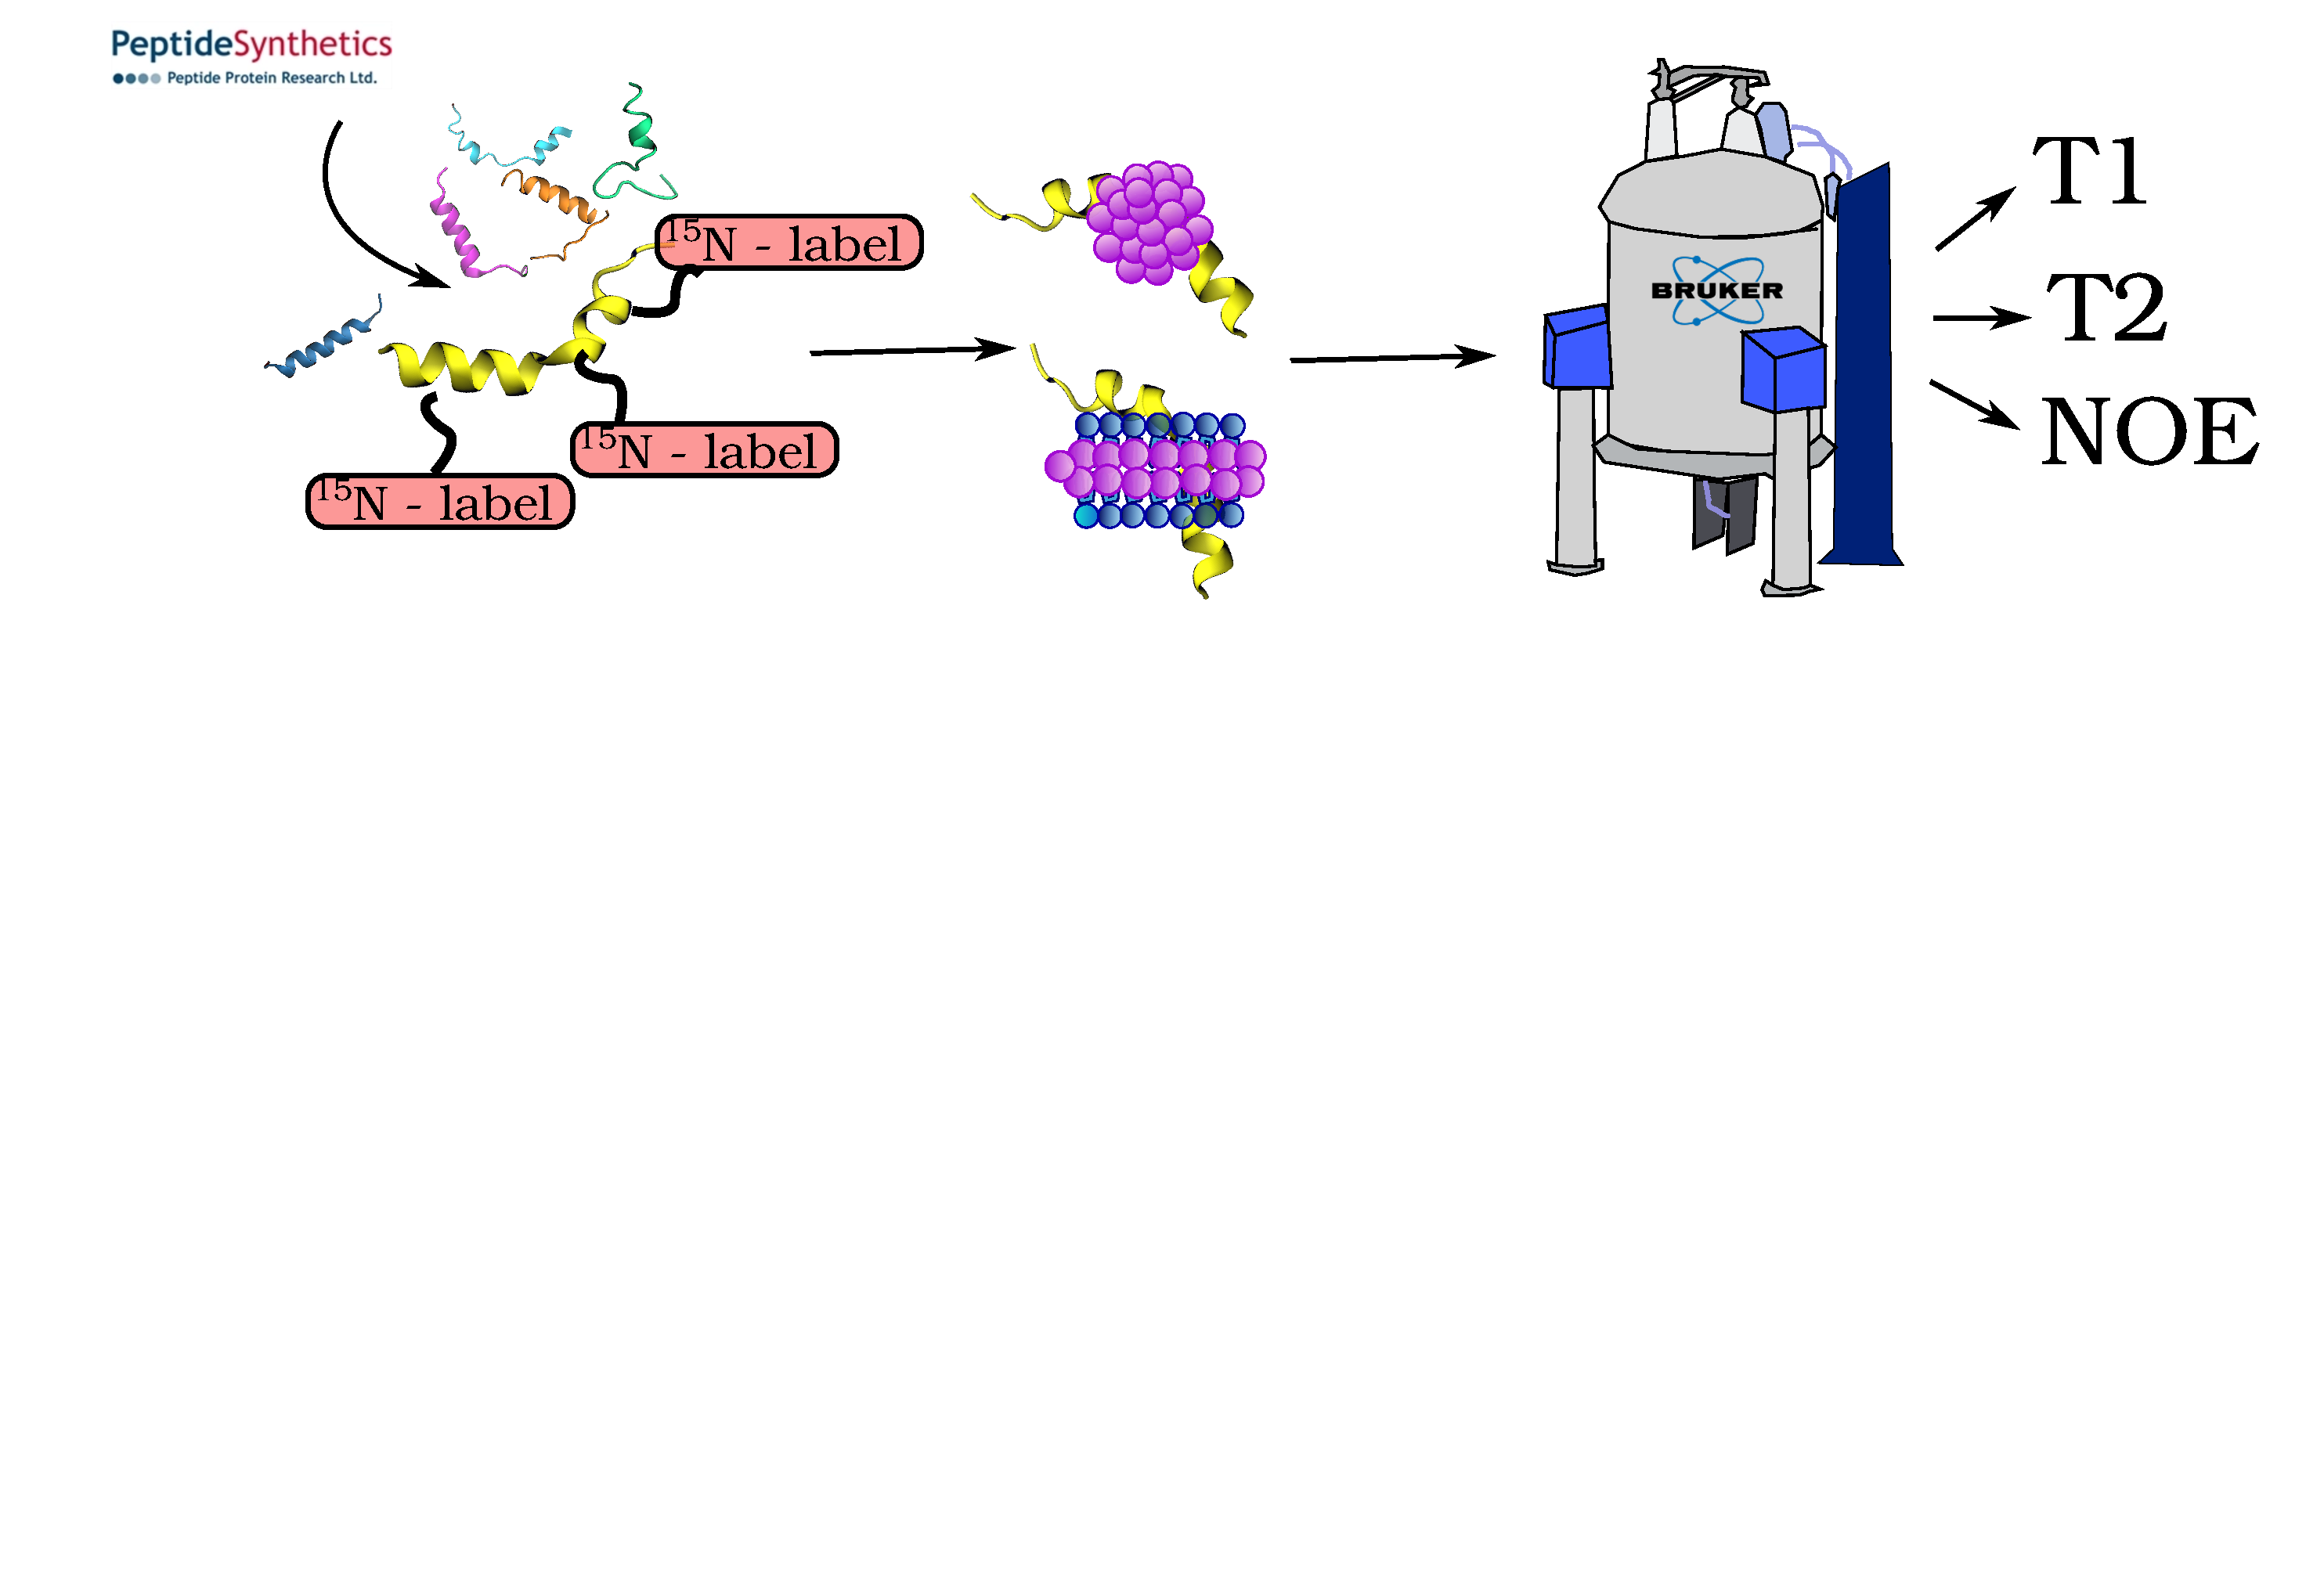
\includegraphics[height=6cm]{what_we_do6.pdf}
\end{center}
\end{frame}


\addtocounter{framenumber}{-1}
\begin{frame}
\begin{center}
\Large{\centering
\textbf{How do we actually do it?} \\}

\vspace{0.5cm}

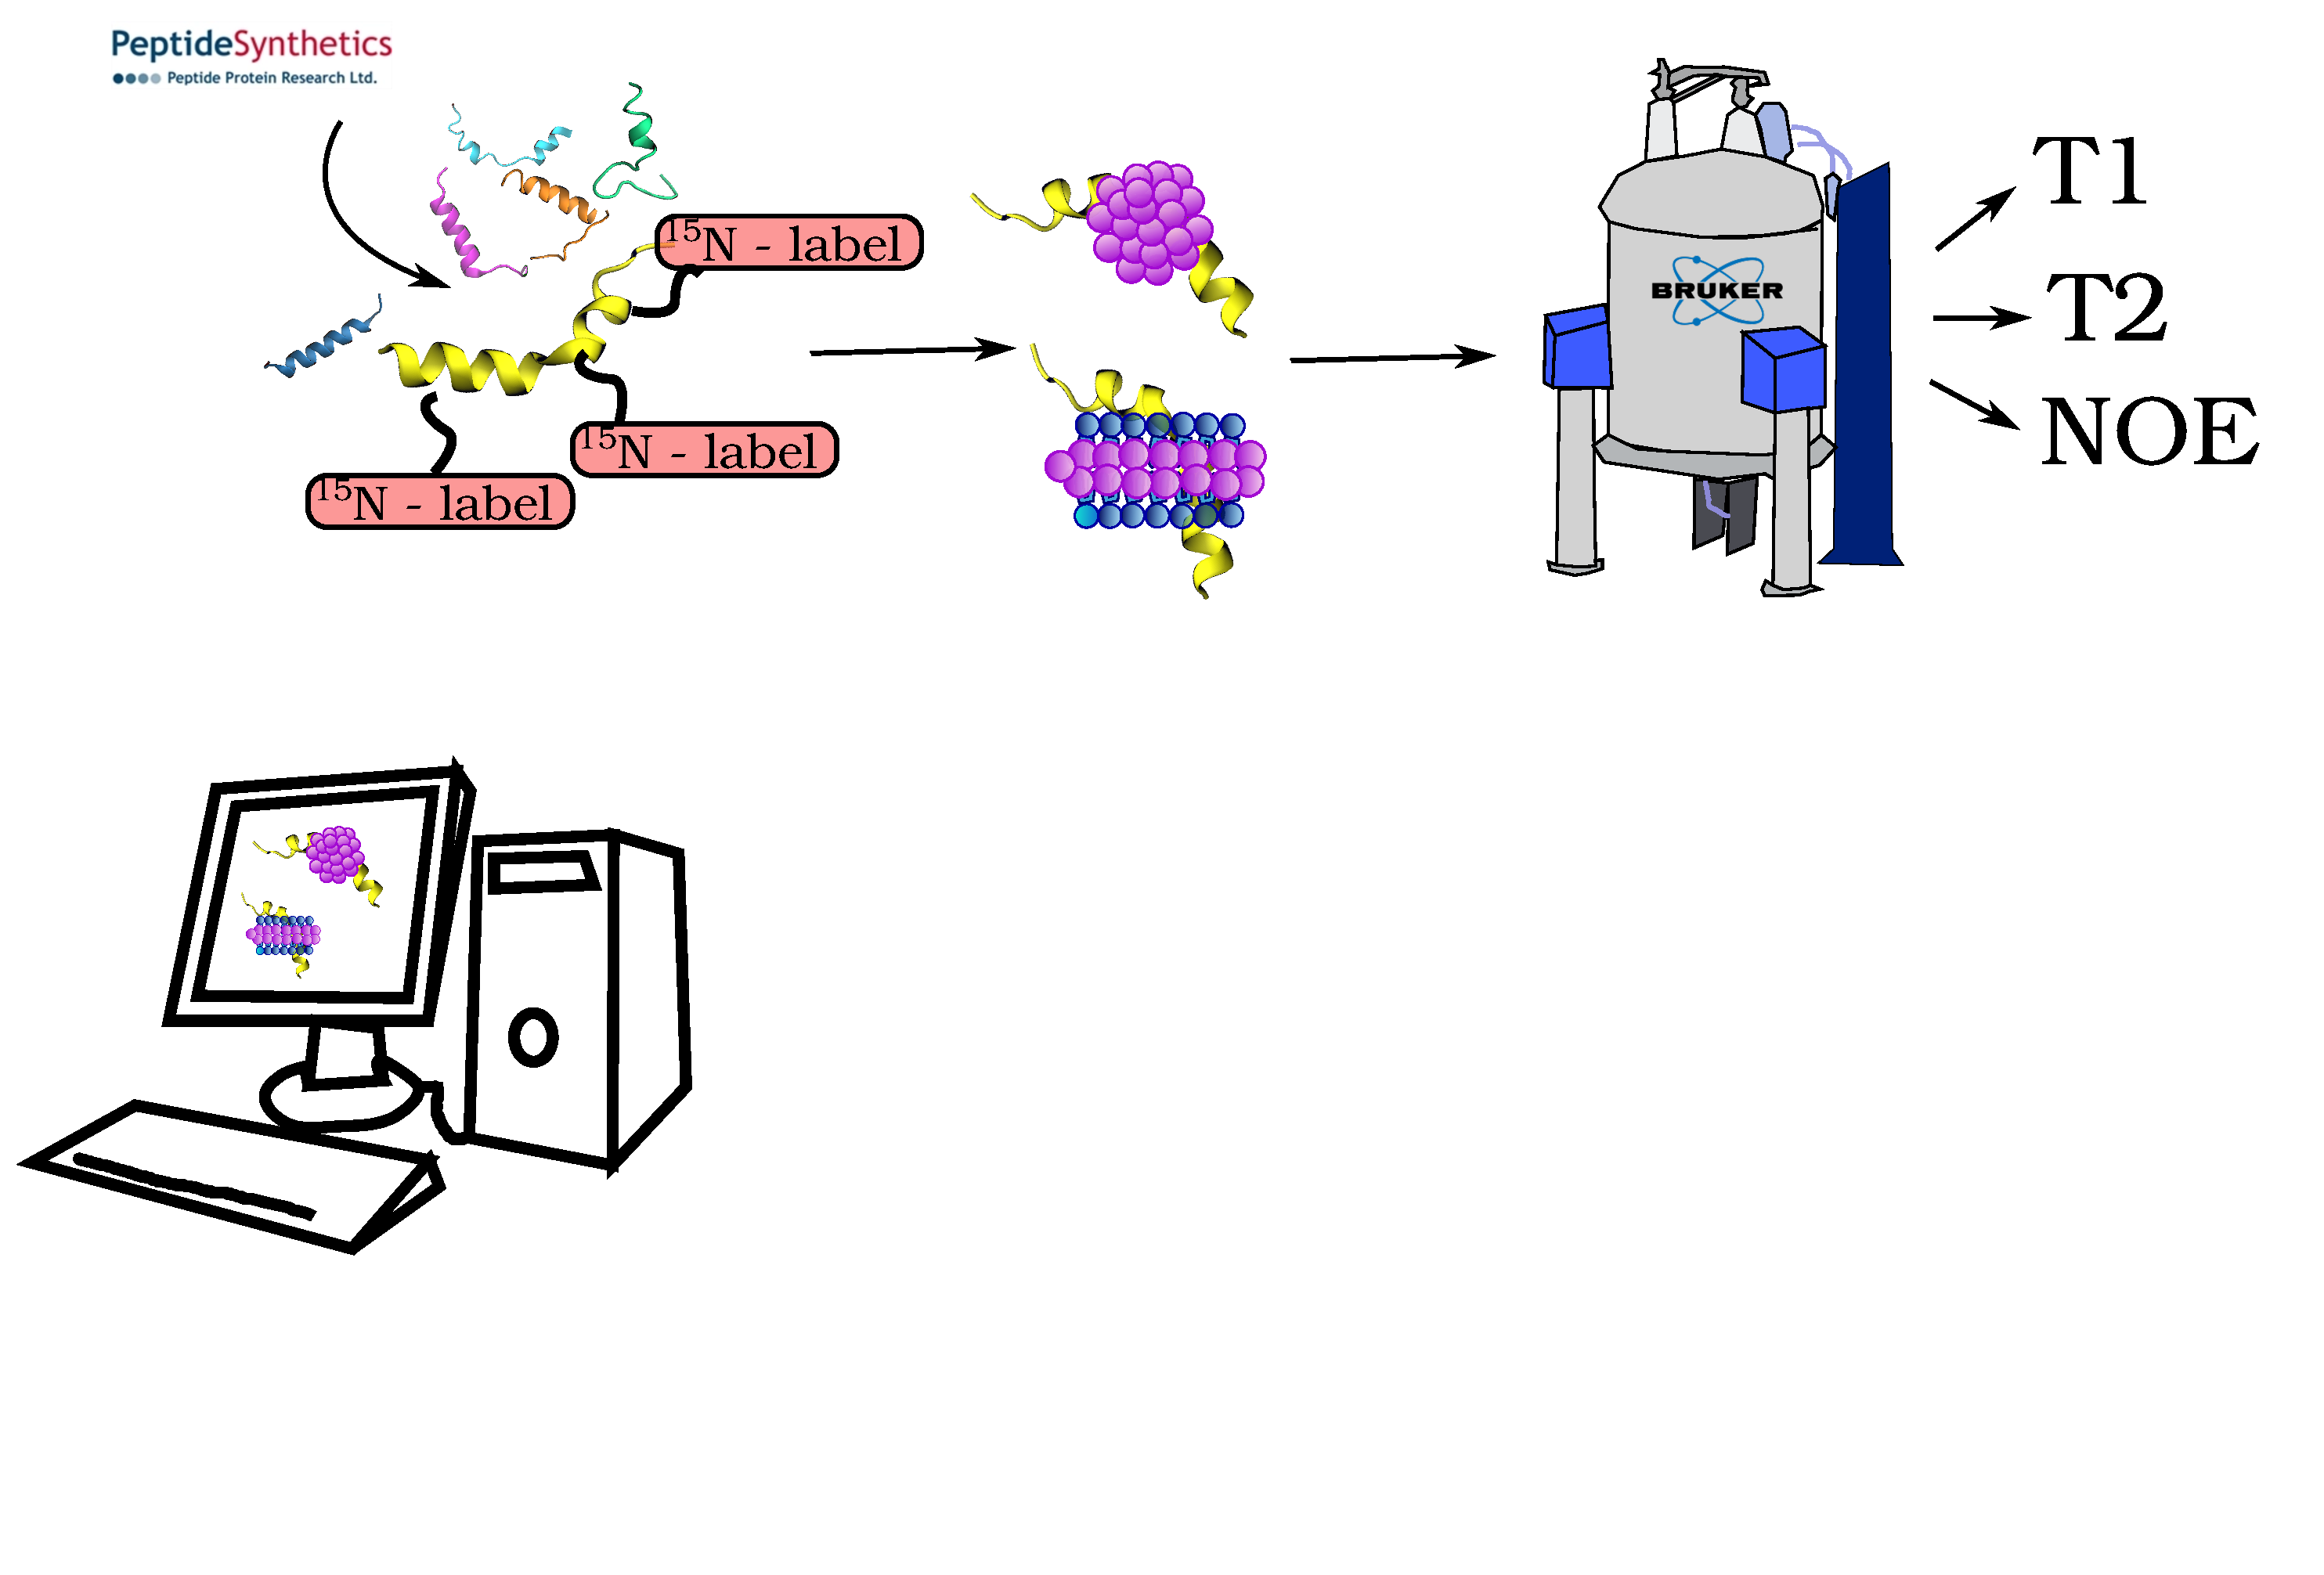
\includegraphics[height=6cm]{what_we_do5.pdf}
\end{center}
\end{frame}


\addtocounter{framenumber}{-1}
\begin{frame}
\begin{center}
\Large{\centering
\textbf{How do we actually do it?} \\}

\vspace{0.5cm}

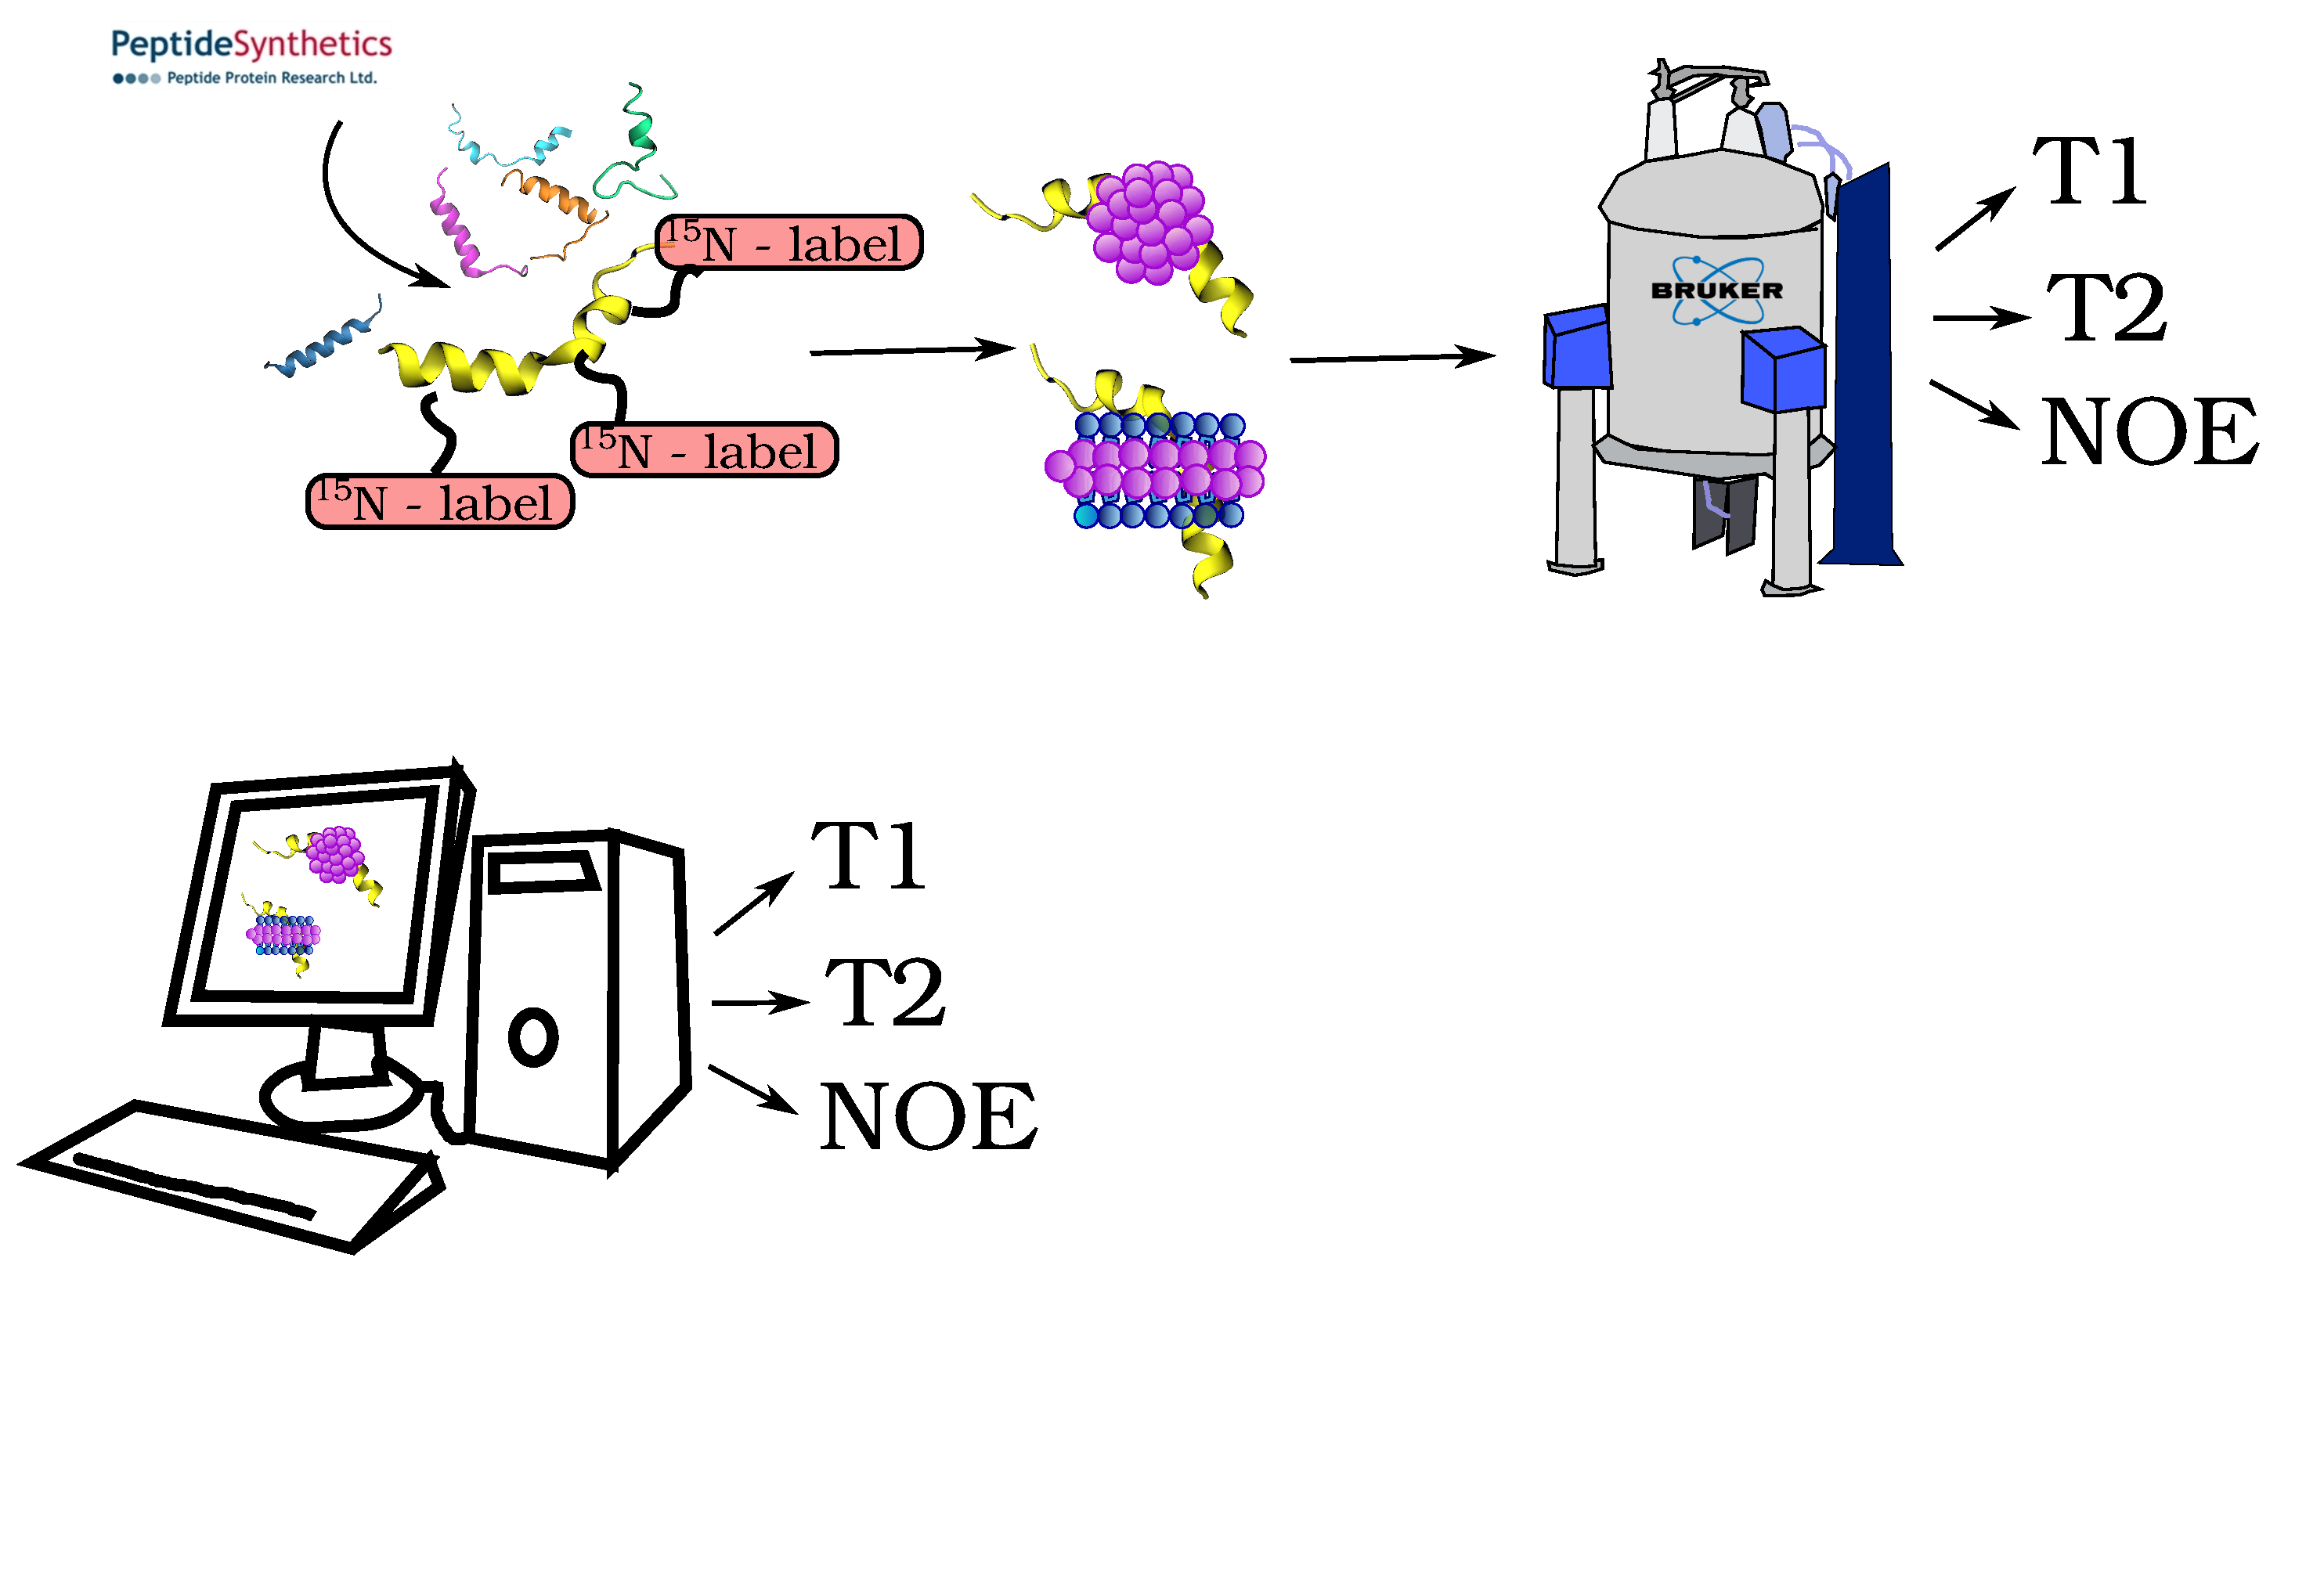
\includegraphics[height=6cm]{what_we_do4.pdf}
\end{center}
\end{frame}


\addtocounter{framenumber}{-1}
\begin{frame}
\begin{center}
\Large{\centering
\textbf{How do we actually do it?} \\}

\vspace{0.5cm}

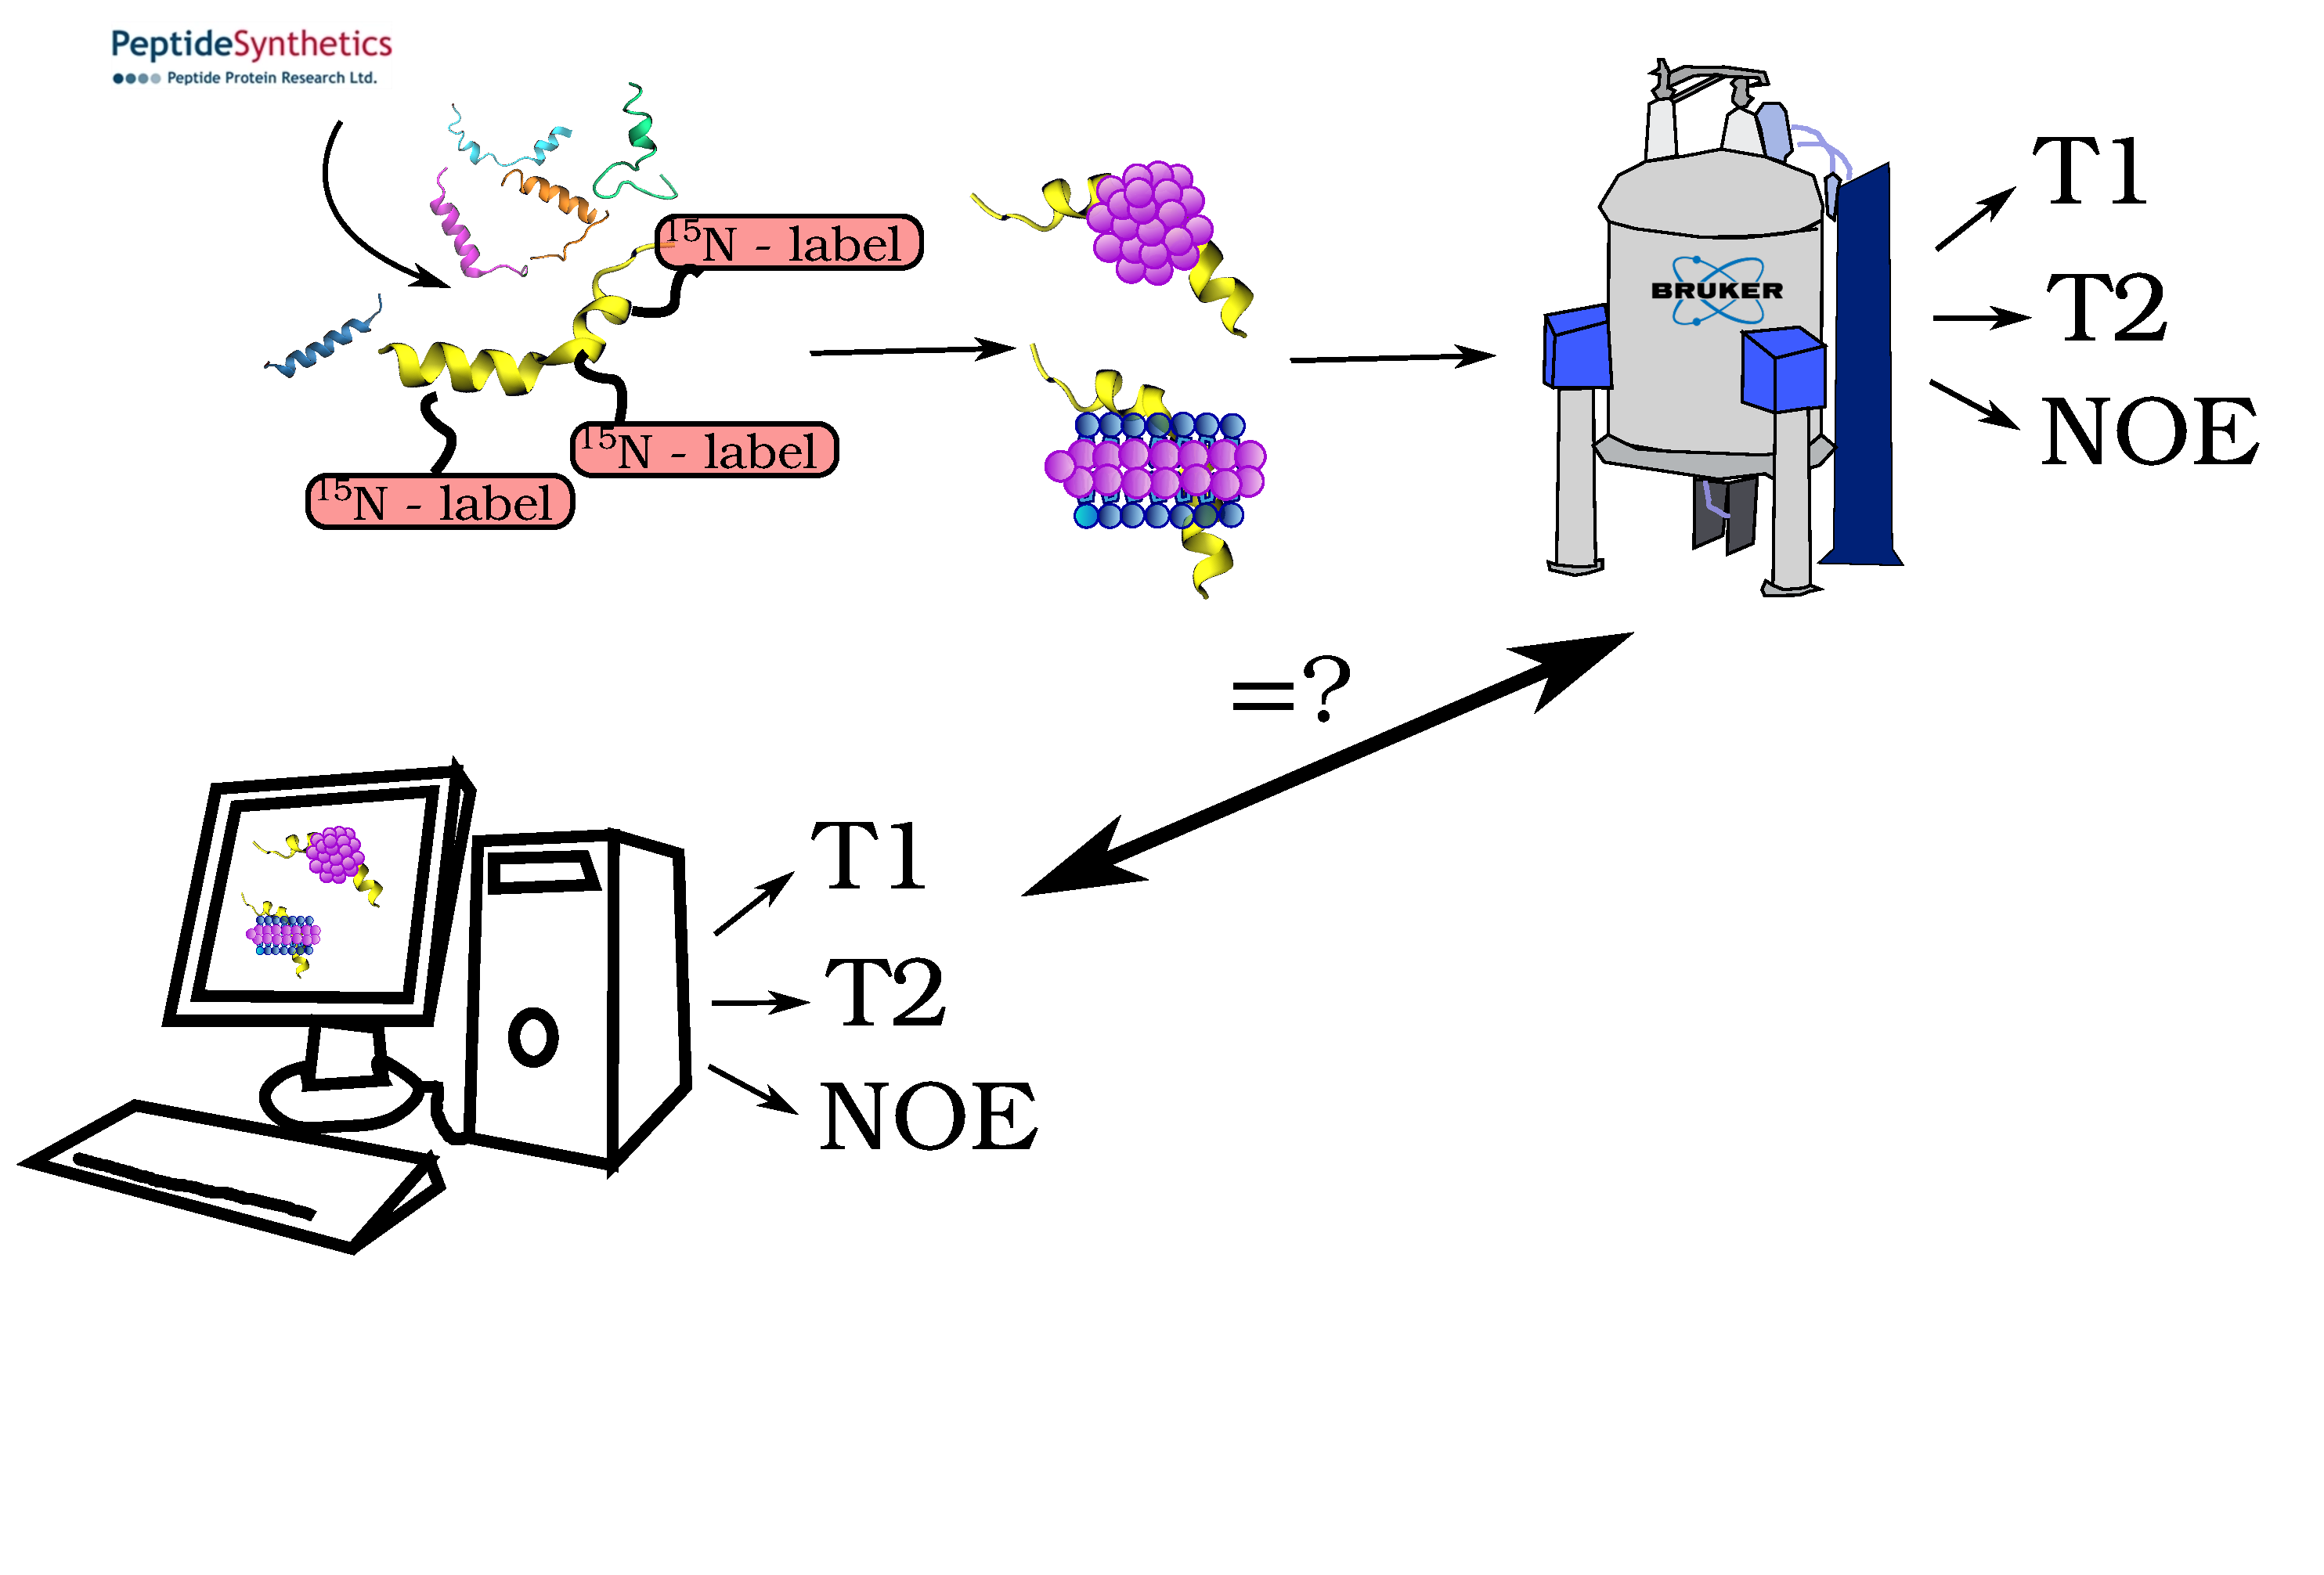
\includegraphics[height=6cm]{what_we_do3.pdf}
\end{center}
\end{frame}


\addtocounter{framenumber}{-1}
\begin{frame}
\begin{center}
\Large{\centering
\textbf{How do we actually do it?} \\}

\vspace{0.5cm}

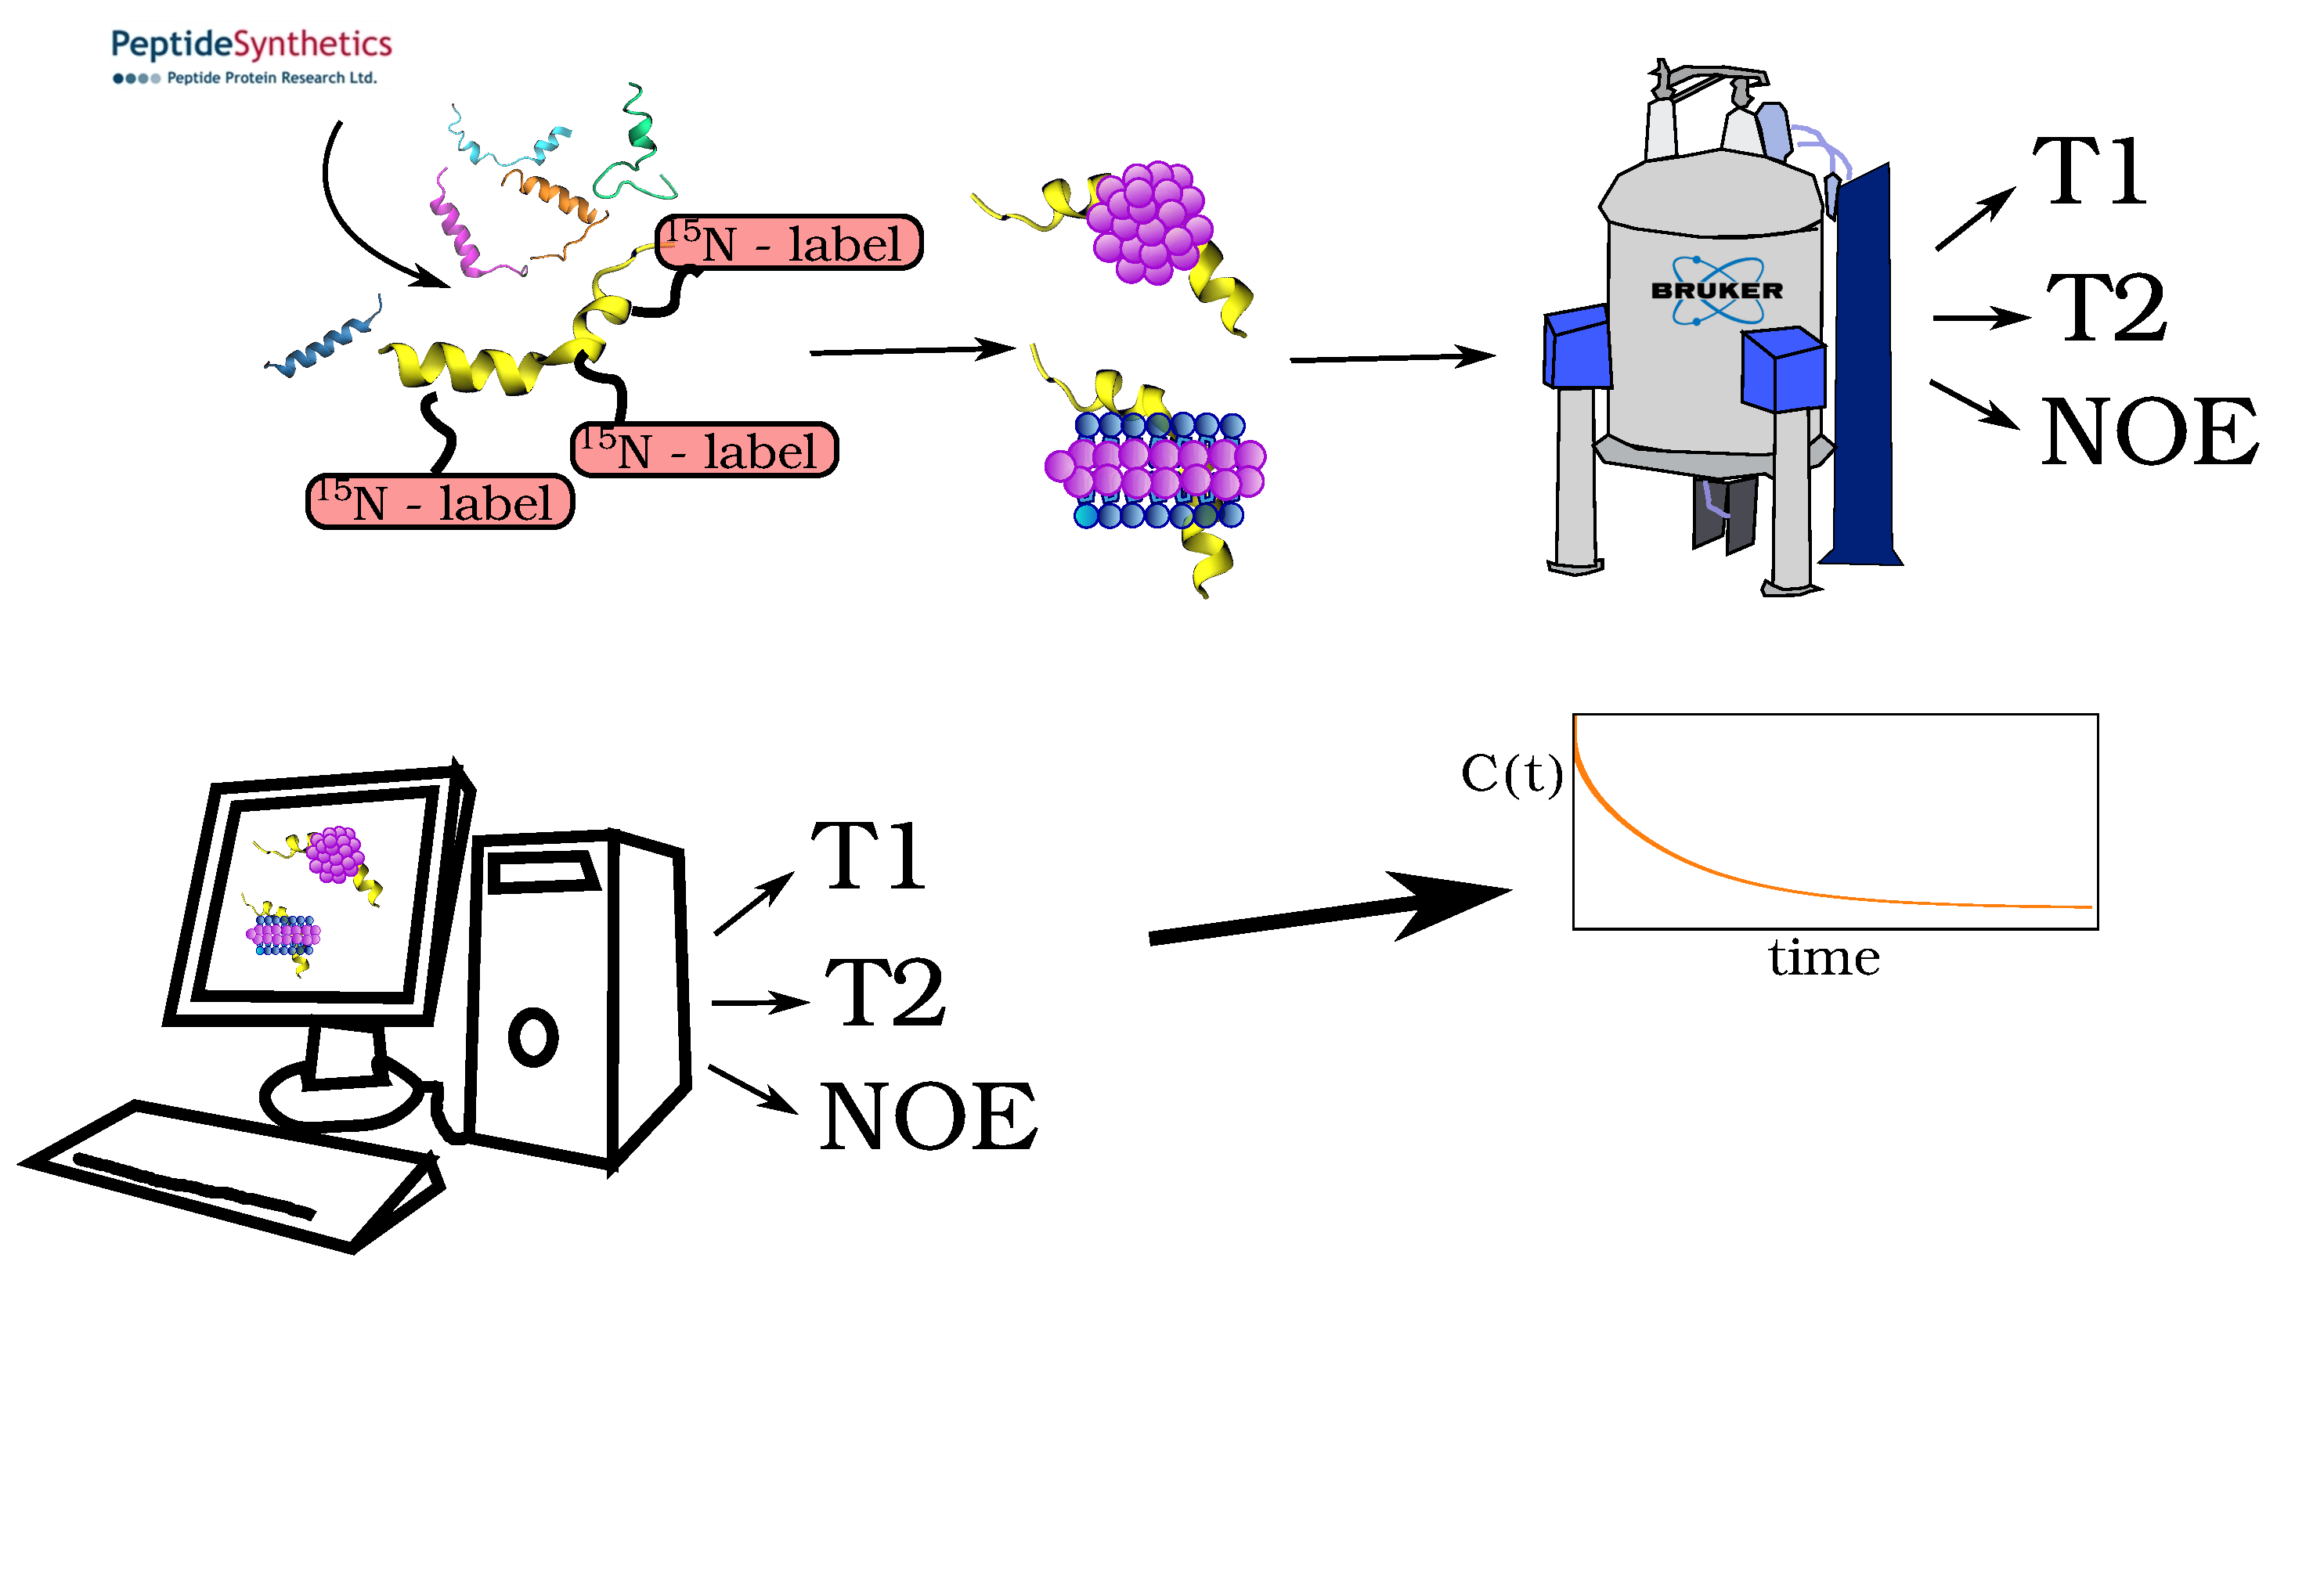
\includegraphics[height=6cm]{what_we_do2.pdf}
\end{center}
\end{frame}


\addtocounter{framenumber}{-1}
\begin{frame}
\begin{center}
\Large{\centering
\textbf{How do we actually do it?} \\}

\vspace{0.5cm}

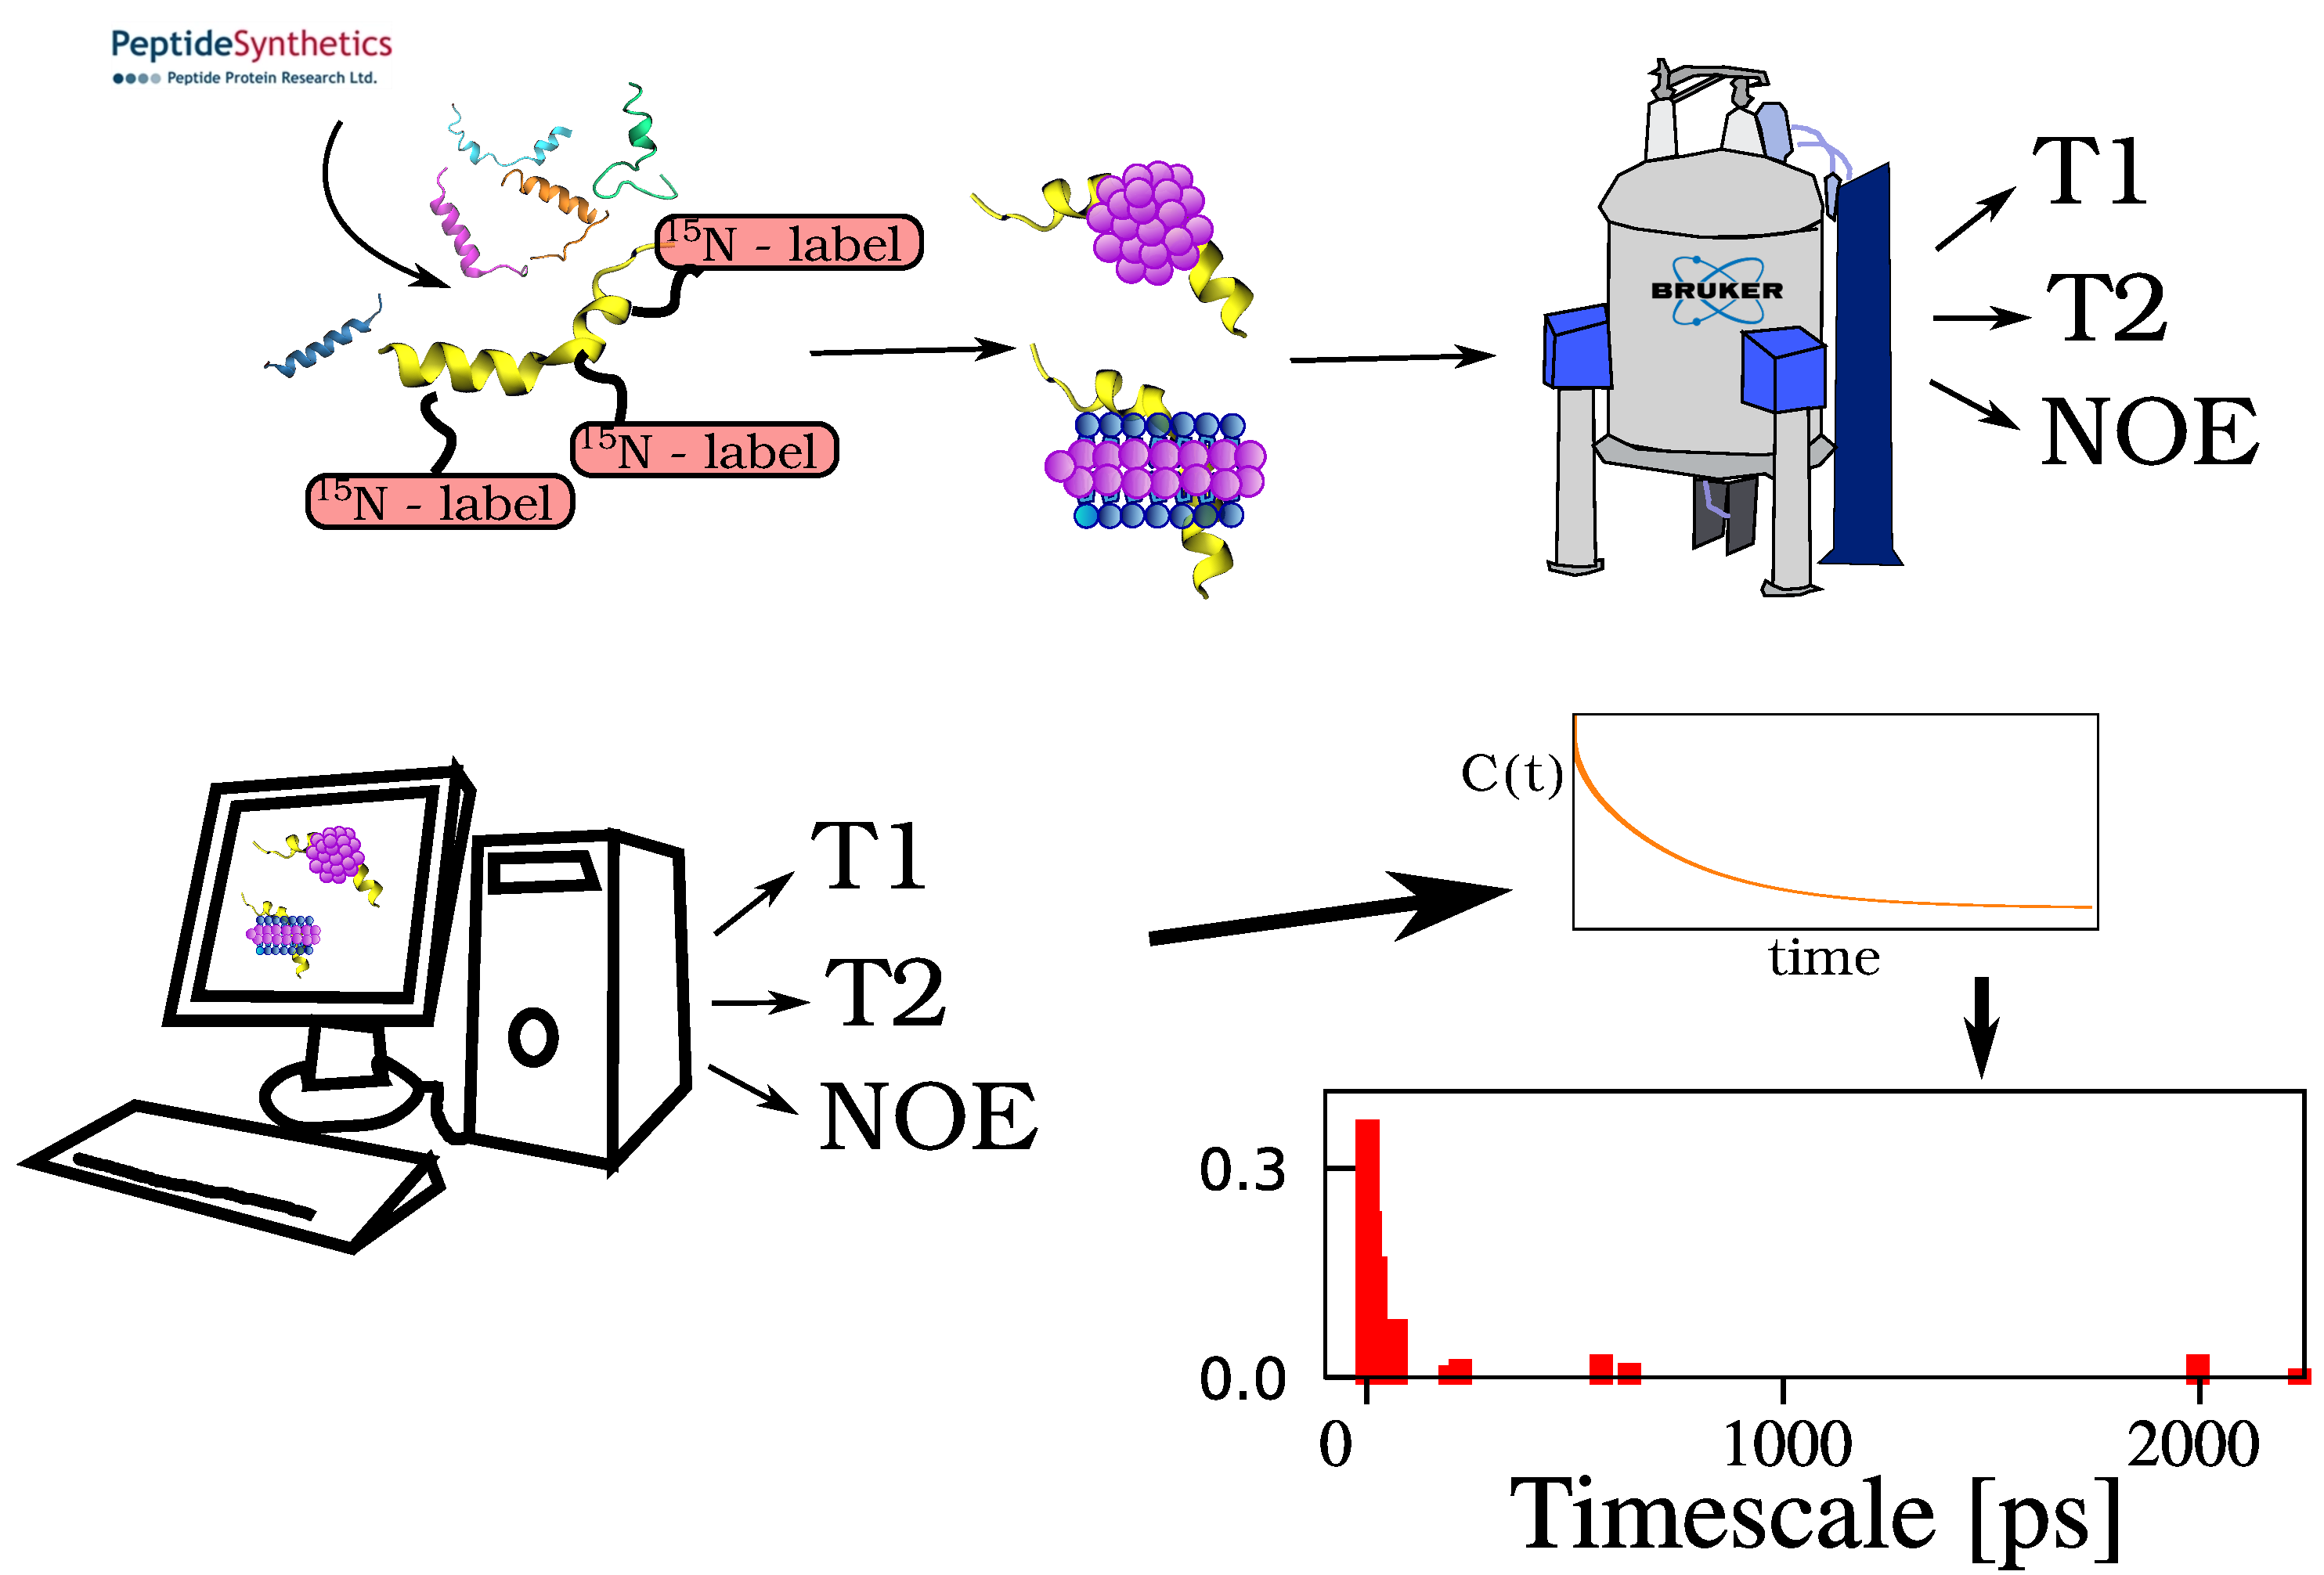
\includegraphics[height=6cm]{what_we_do1.pdf}
\end{center}
\end{frame}



\subsection{TonB}


\begin{frame}
\begin{center}
\Large{\centering
\textbf{Succesfull case: TonB} \\}

\vspace{0.5cm}

Yet to be done - Our approach shad a light on the conformational ensamble of the protein

\end{center}
\end{frame}


%\begin{frame}
%\LARGE{\centering
%\textbf{Outline} \\
%\begin{center}
% 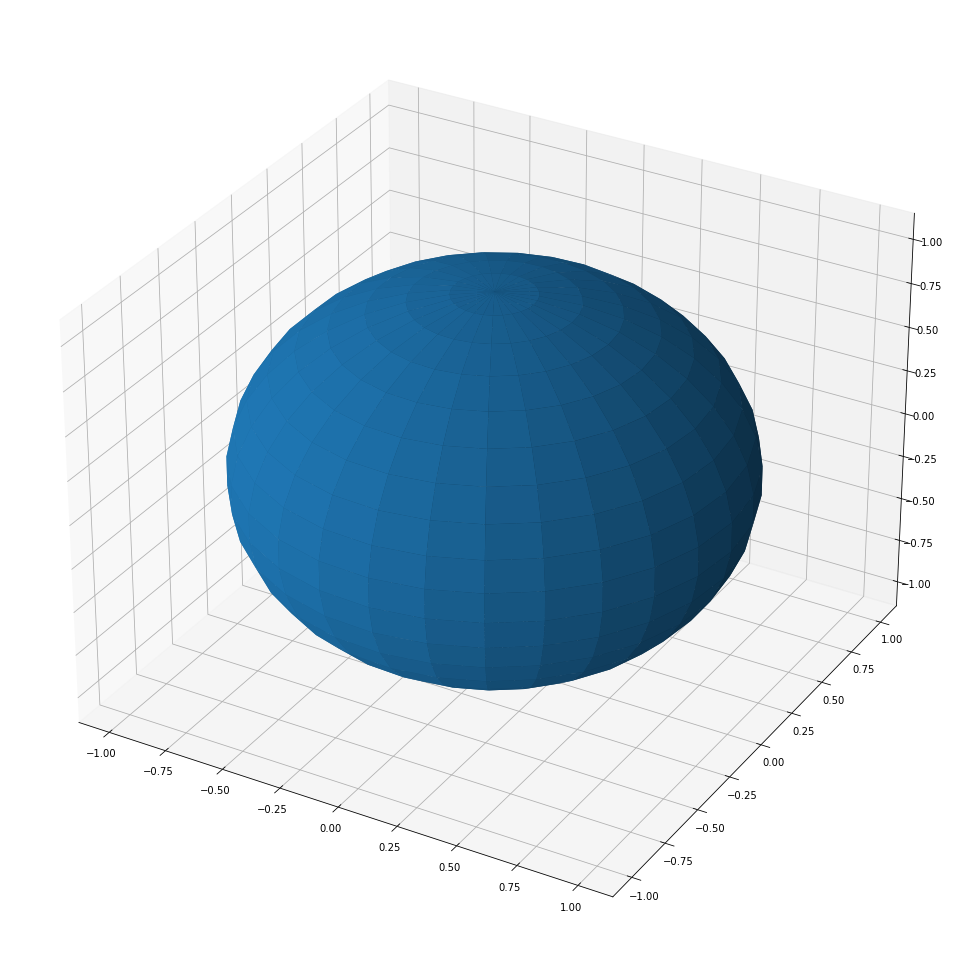
\includegraphics[height=5cm]{kolo.png}
%\end{center}
%}
%{\tiny http://www.clker.com/clipart-animal-cell-3.html }
%\end{frame}





\begin{frame}
\begin{center}
\Large{\centering
\textbf{What do T1, T2 and NOE tell us?} \\}

\includegraphics[height=5cm]{dynam4.pdf}
\end{center}
\end{frame}


\addtocounter{framenumber}{-1}
\begin{frame}
\begin{center}
\Large{\centering
\textbf{What do T1, T2 and NOE tell us?} \\}
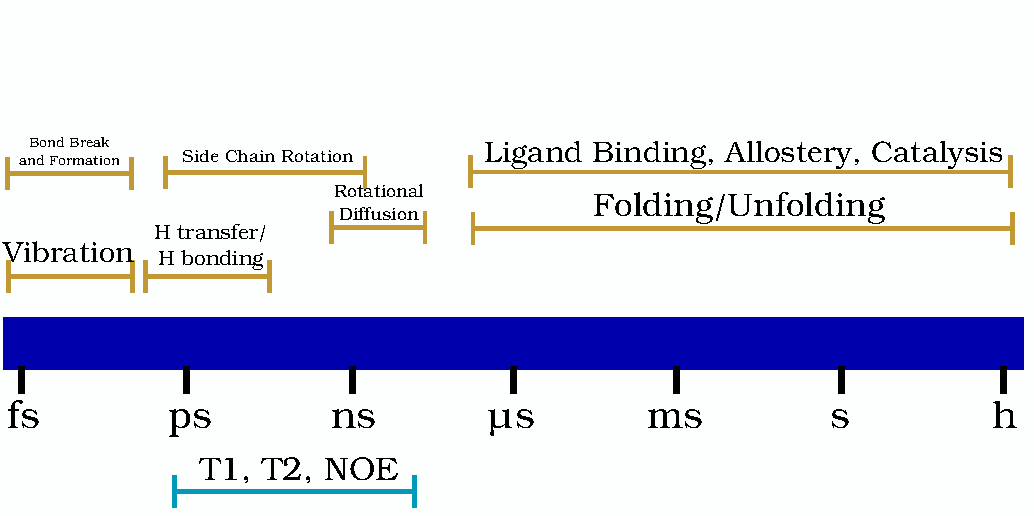
\includegraphics[height=5cm]{dynam0.pdf}
\end{center}
\end{frame}

\addtocounter{framenumber}{-1}
\begin{frame}
\begin{center}
\Large{\centering
\textbf{What do T1, T2 and NOE tell us?} \\}
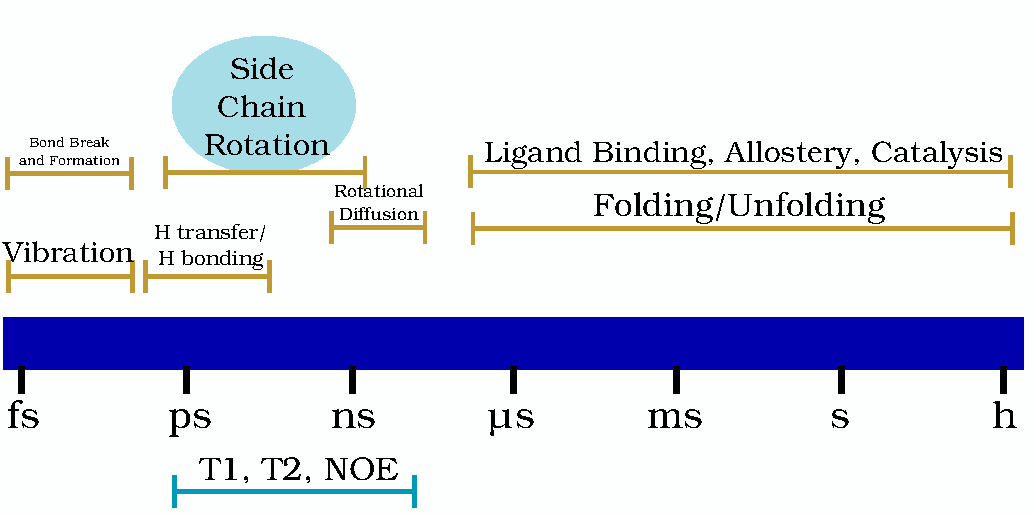
\includegraphics[height=5cm]{dynam1.pdf}
\end{center}
\end{frame}


\addtocounter{framenumber}{-1}
\begin{frame}
\begin{center}
\Large{\centering
\textbf{What do T1, T2 and NOE tell us?} \\}
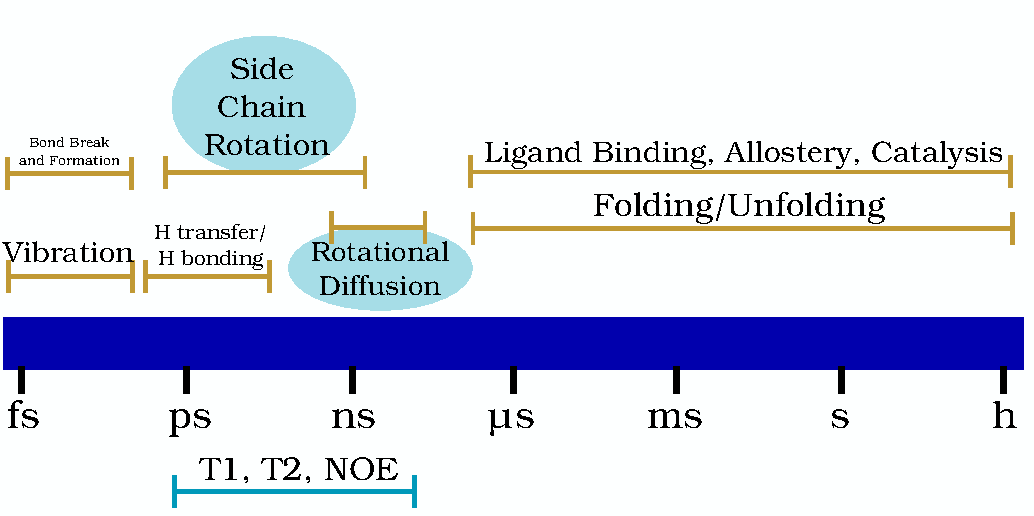
\includegraphics[height=5cm]{dynam2.pdf}
\end{center}
\end{frame}


\addtocounter{framenumber}{-1}
\begin{frame}
\begin{center}
\Large{\centering
\textbf{What do T1, T2 and NOE tell us?} \\}
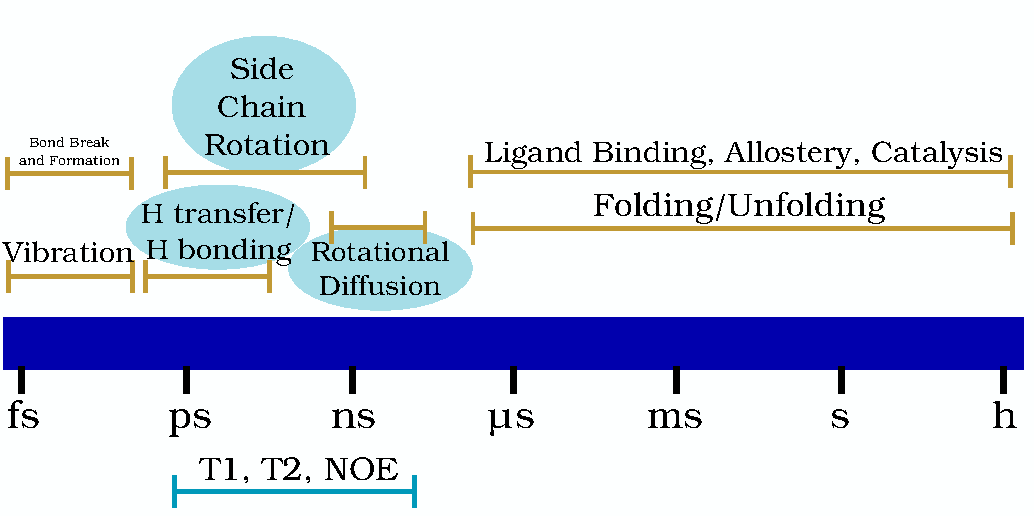
\includegraphics[height=5cm]{dynam3.pdf}
\end{center}
\end{frame}


\subsection{samples}


\begin{frame}
\begin{center}
\Large{\centering
\textbf{What samples can be prepared?} \\}

\vspace{0.5cm}


\includegraphics[height=6cm]{plots/samples0.pdf}
\end{center}
\end{frame}

\addtocounter{framenumber}{-1}
\begin{frame}
\begin{center}
\Large{\centering
\textbf{What samples can be prepared?} \\}

\vspace{0.5cm}

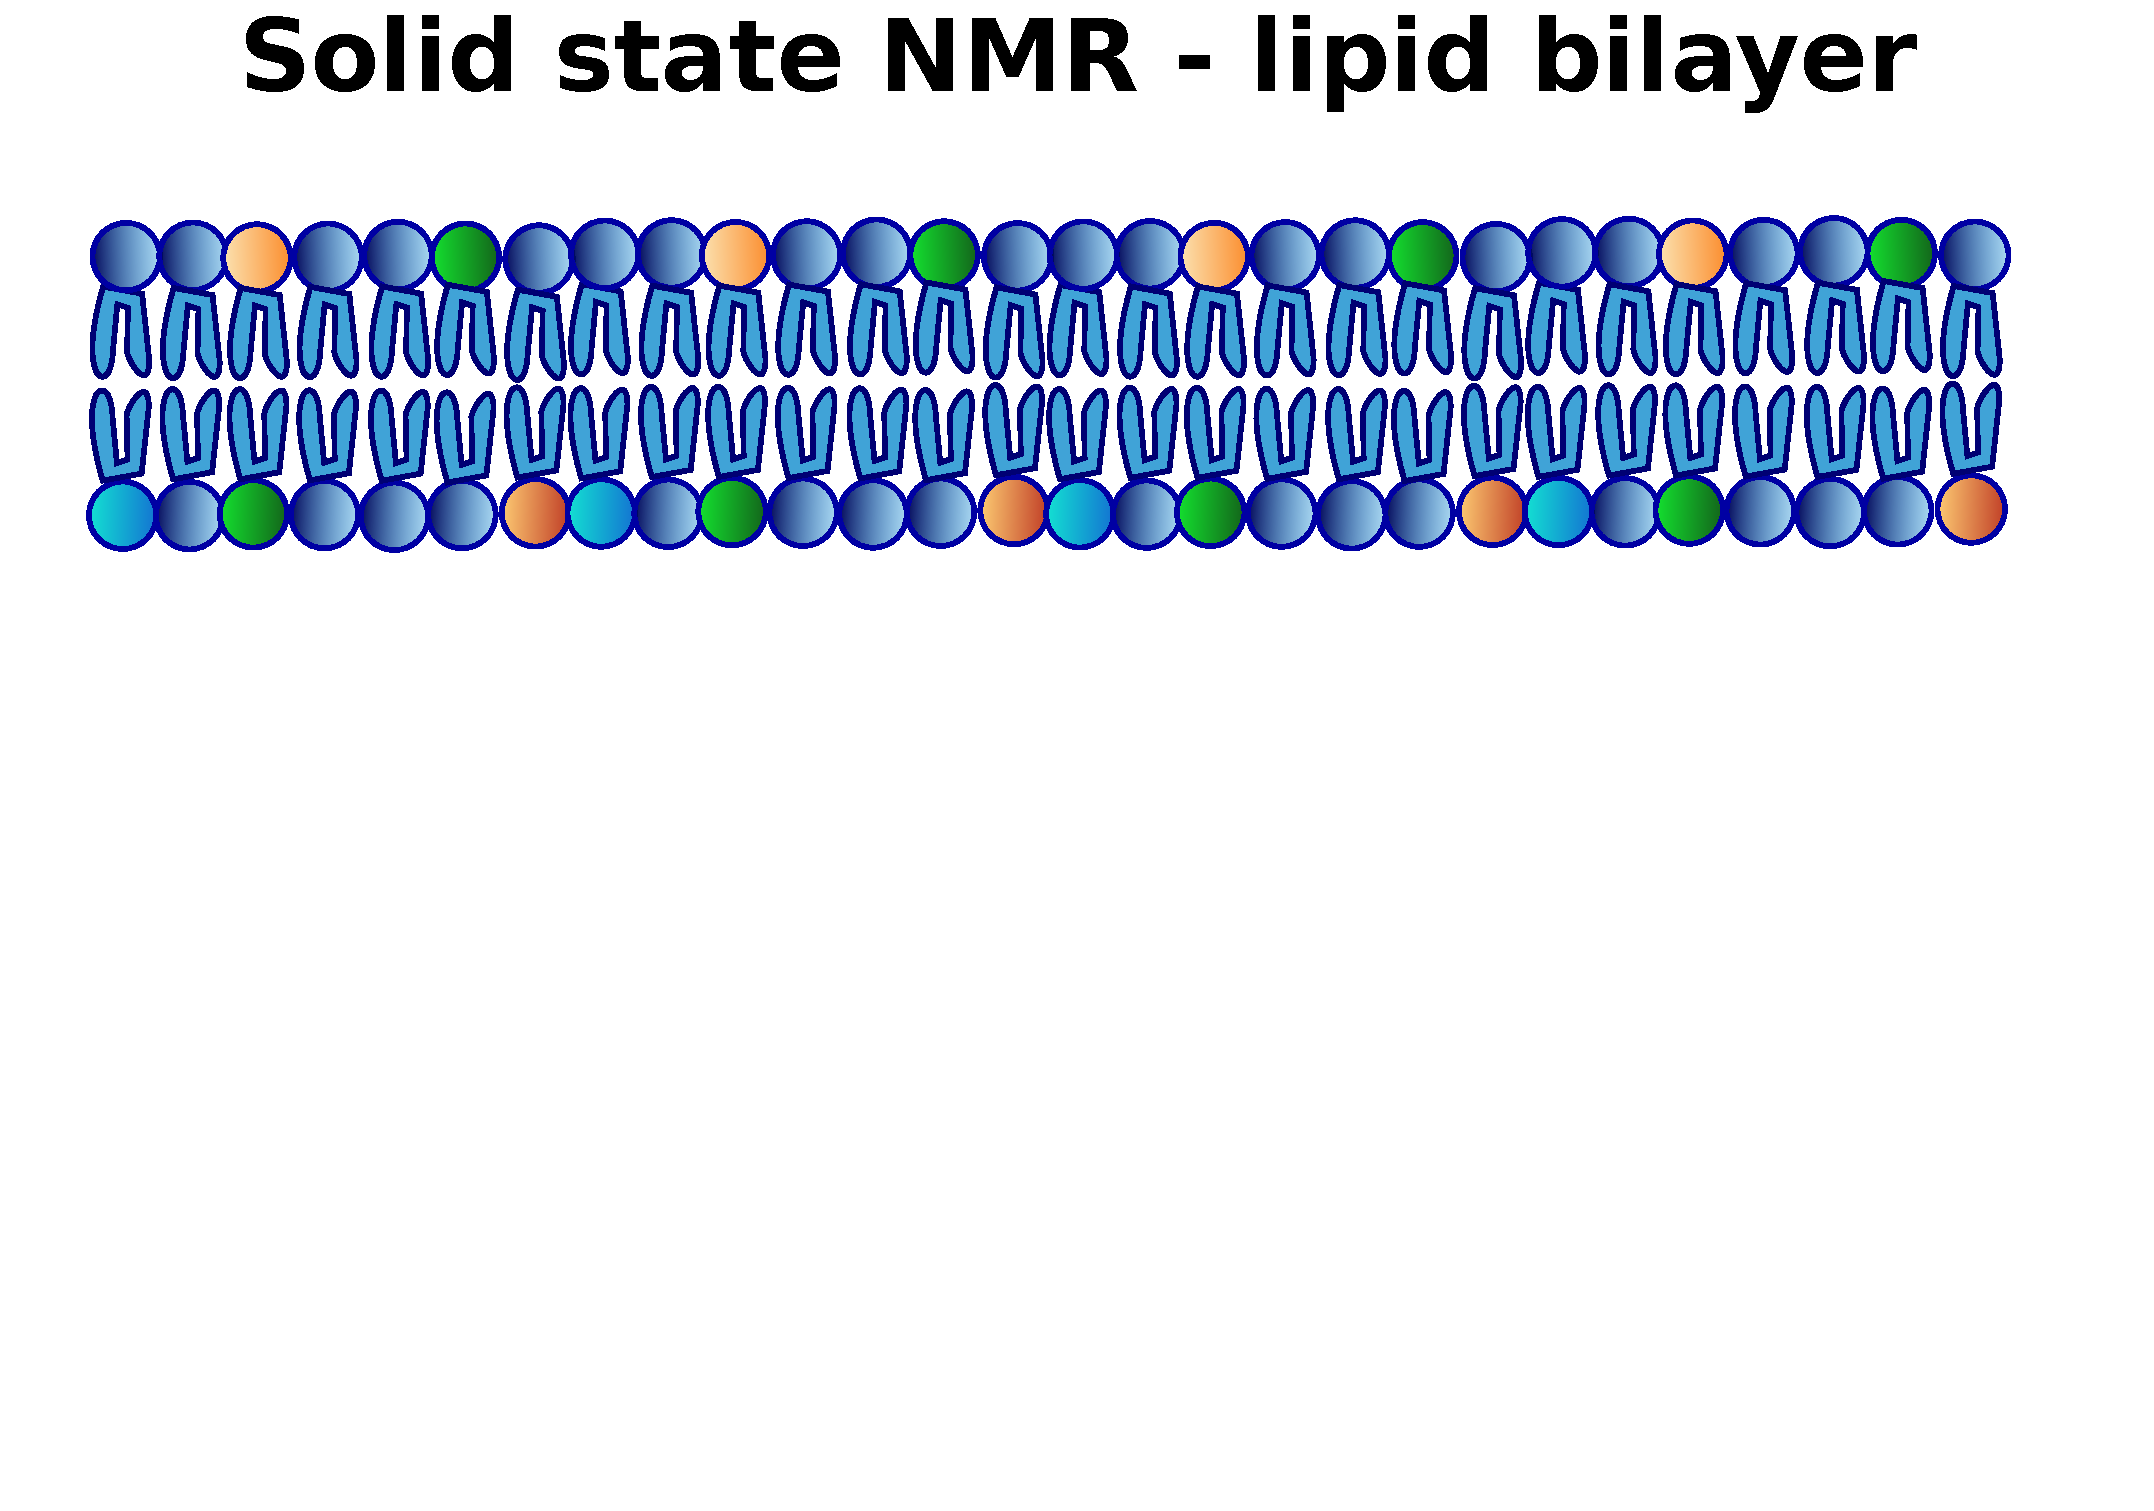
\includegraphics[height=6cm]{plots/samples9.pdf}
\end{center}
\end{frame}


\addtocounter{framenumber}{-1}
\begin{frame}
\begin{center}
\Large{\centering
\textbf{What samples can be prepared?} \\}

\vspace{0.5cm}

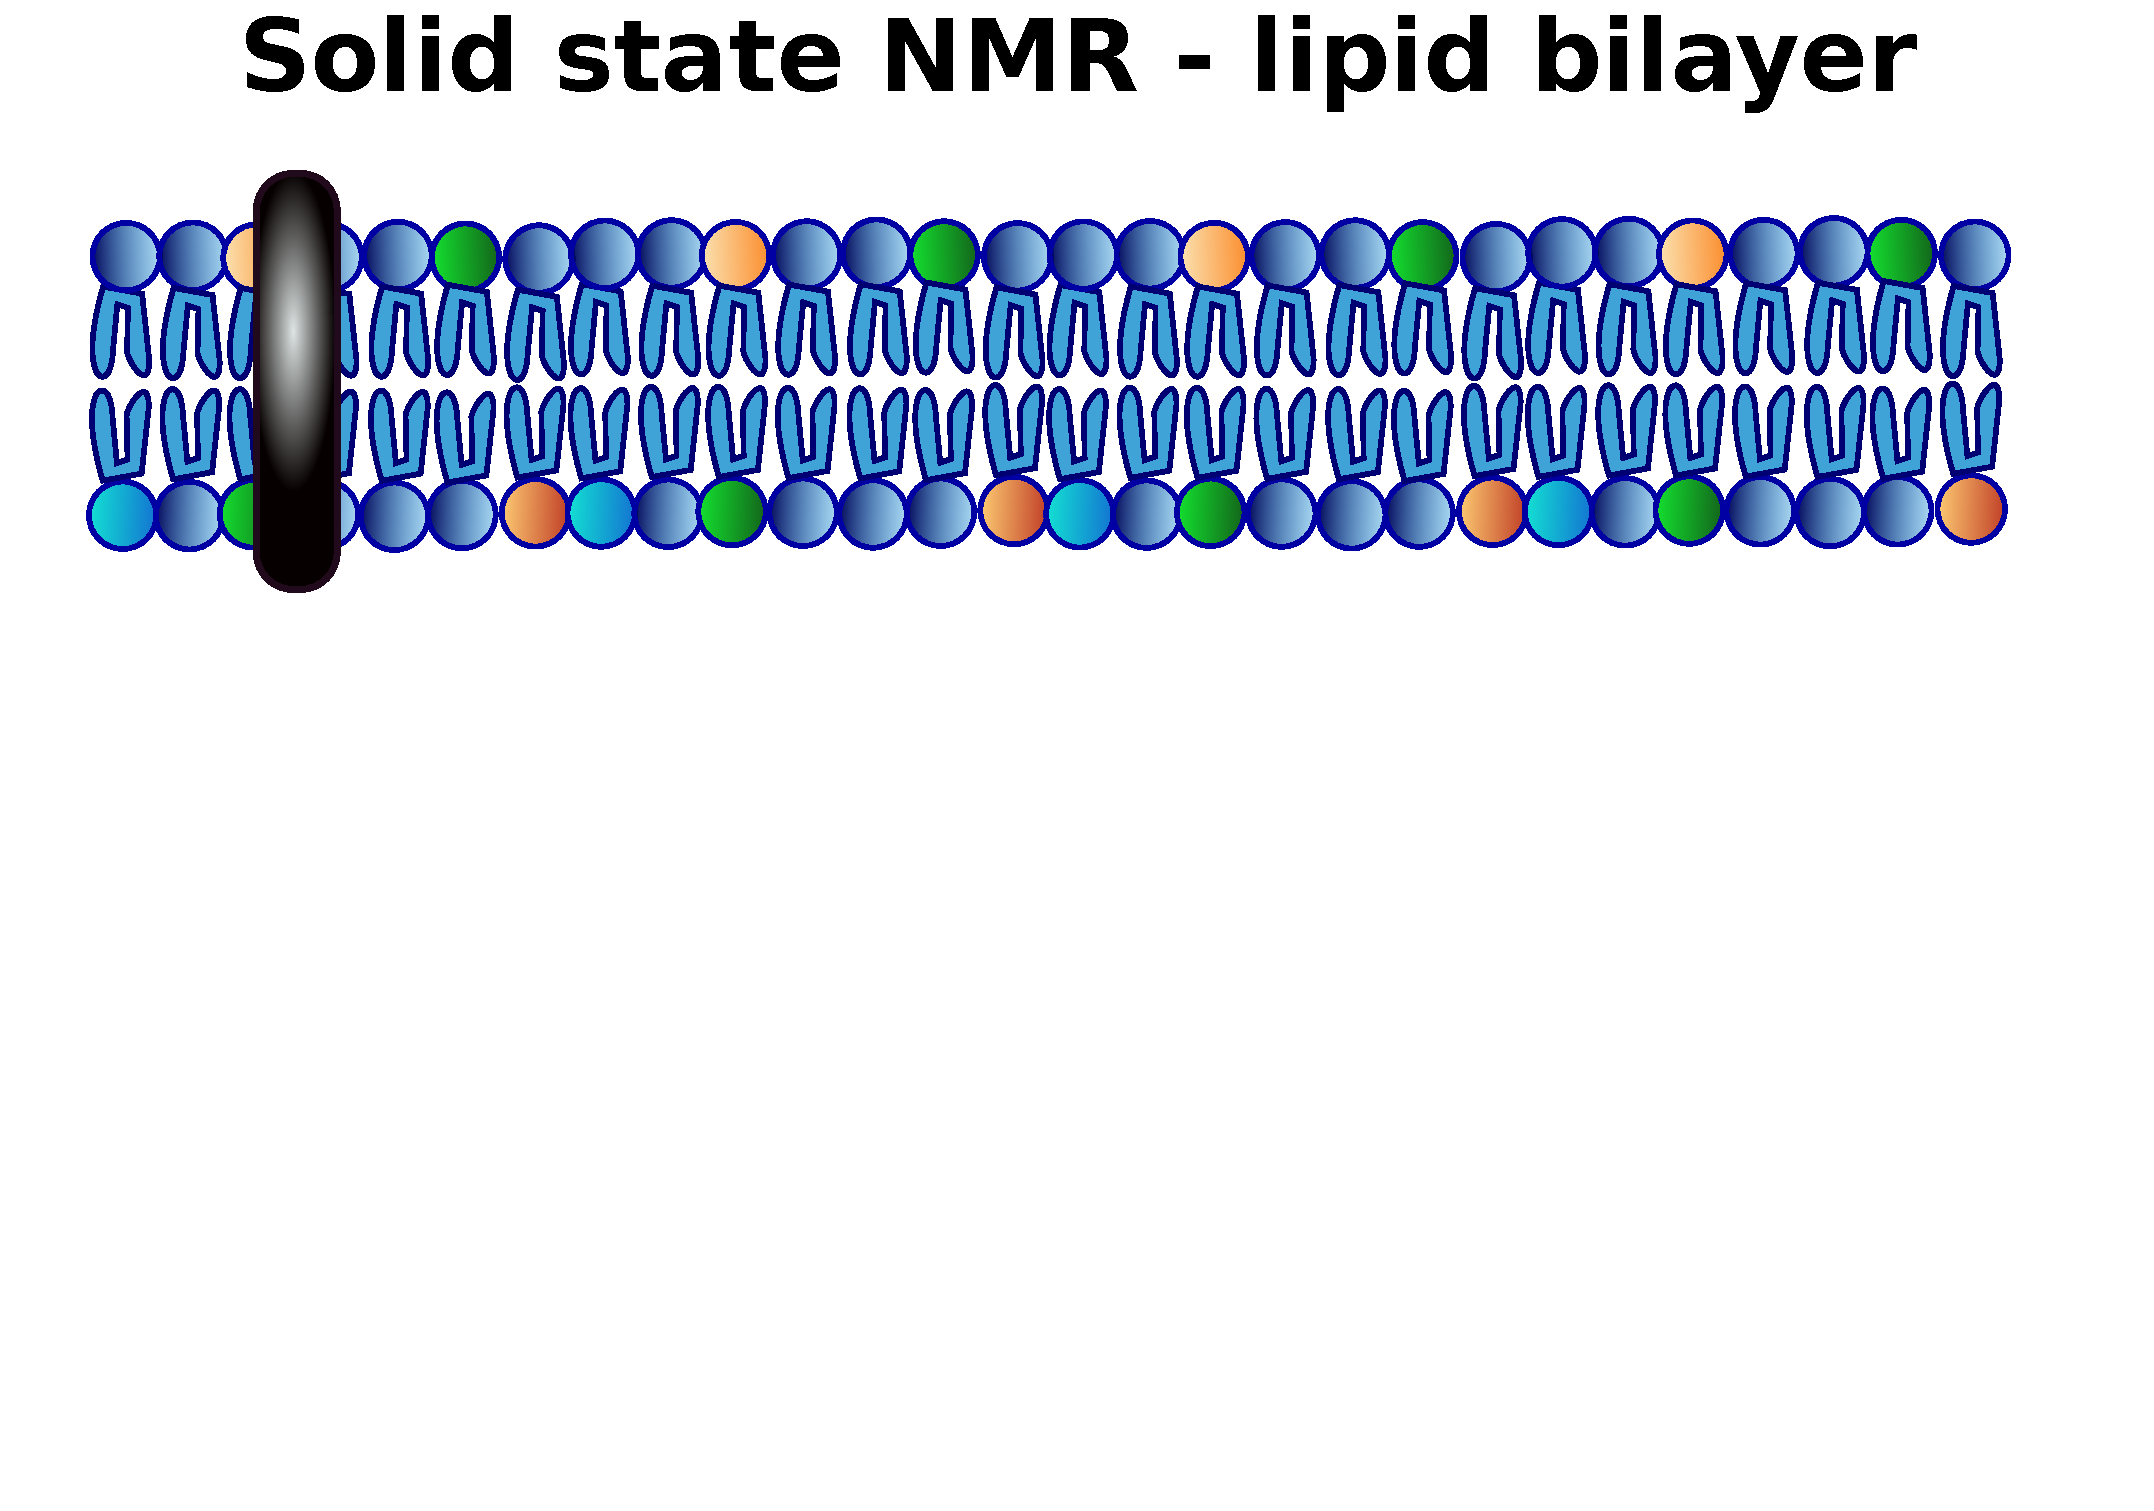
\includegraphics[height=6cm]{plots/samples8.pdf}
\end{center}
\end{frame}



\addtocounter{framenumber}{-1}
\begin{frame}
\begin{center}
\Large{\centering
\textbf{What samples can be prepared?} \\}

\vspace{0.5cm}

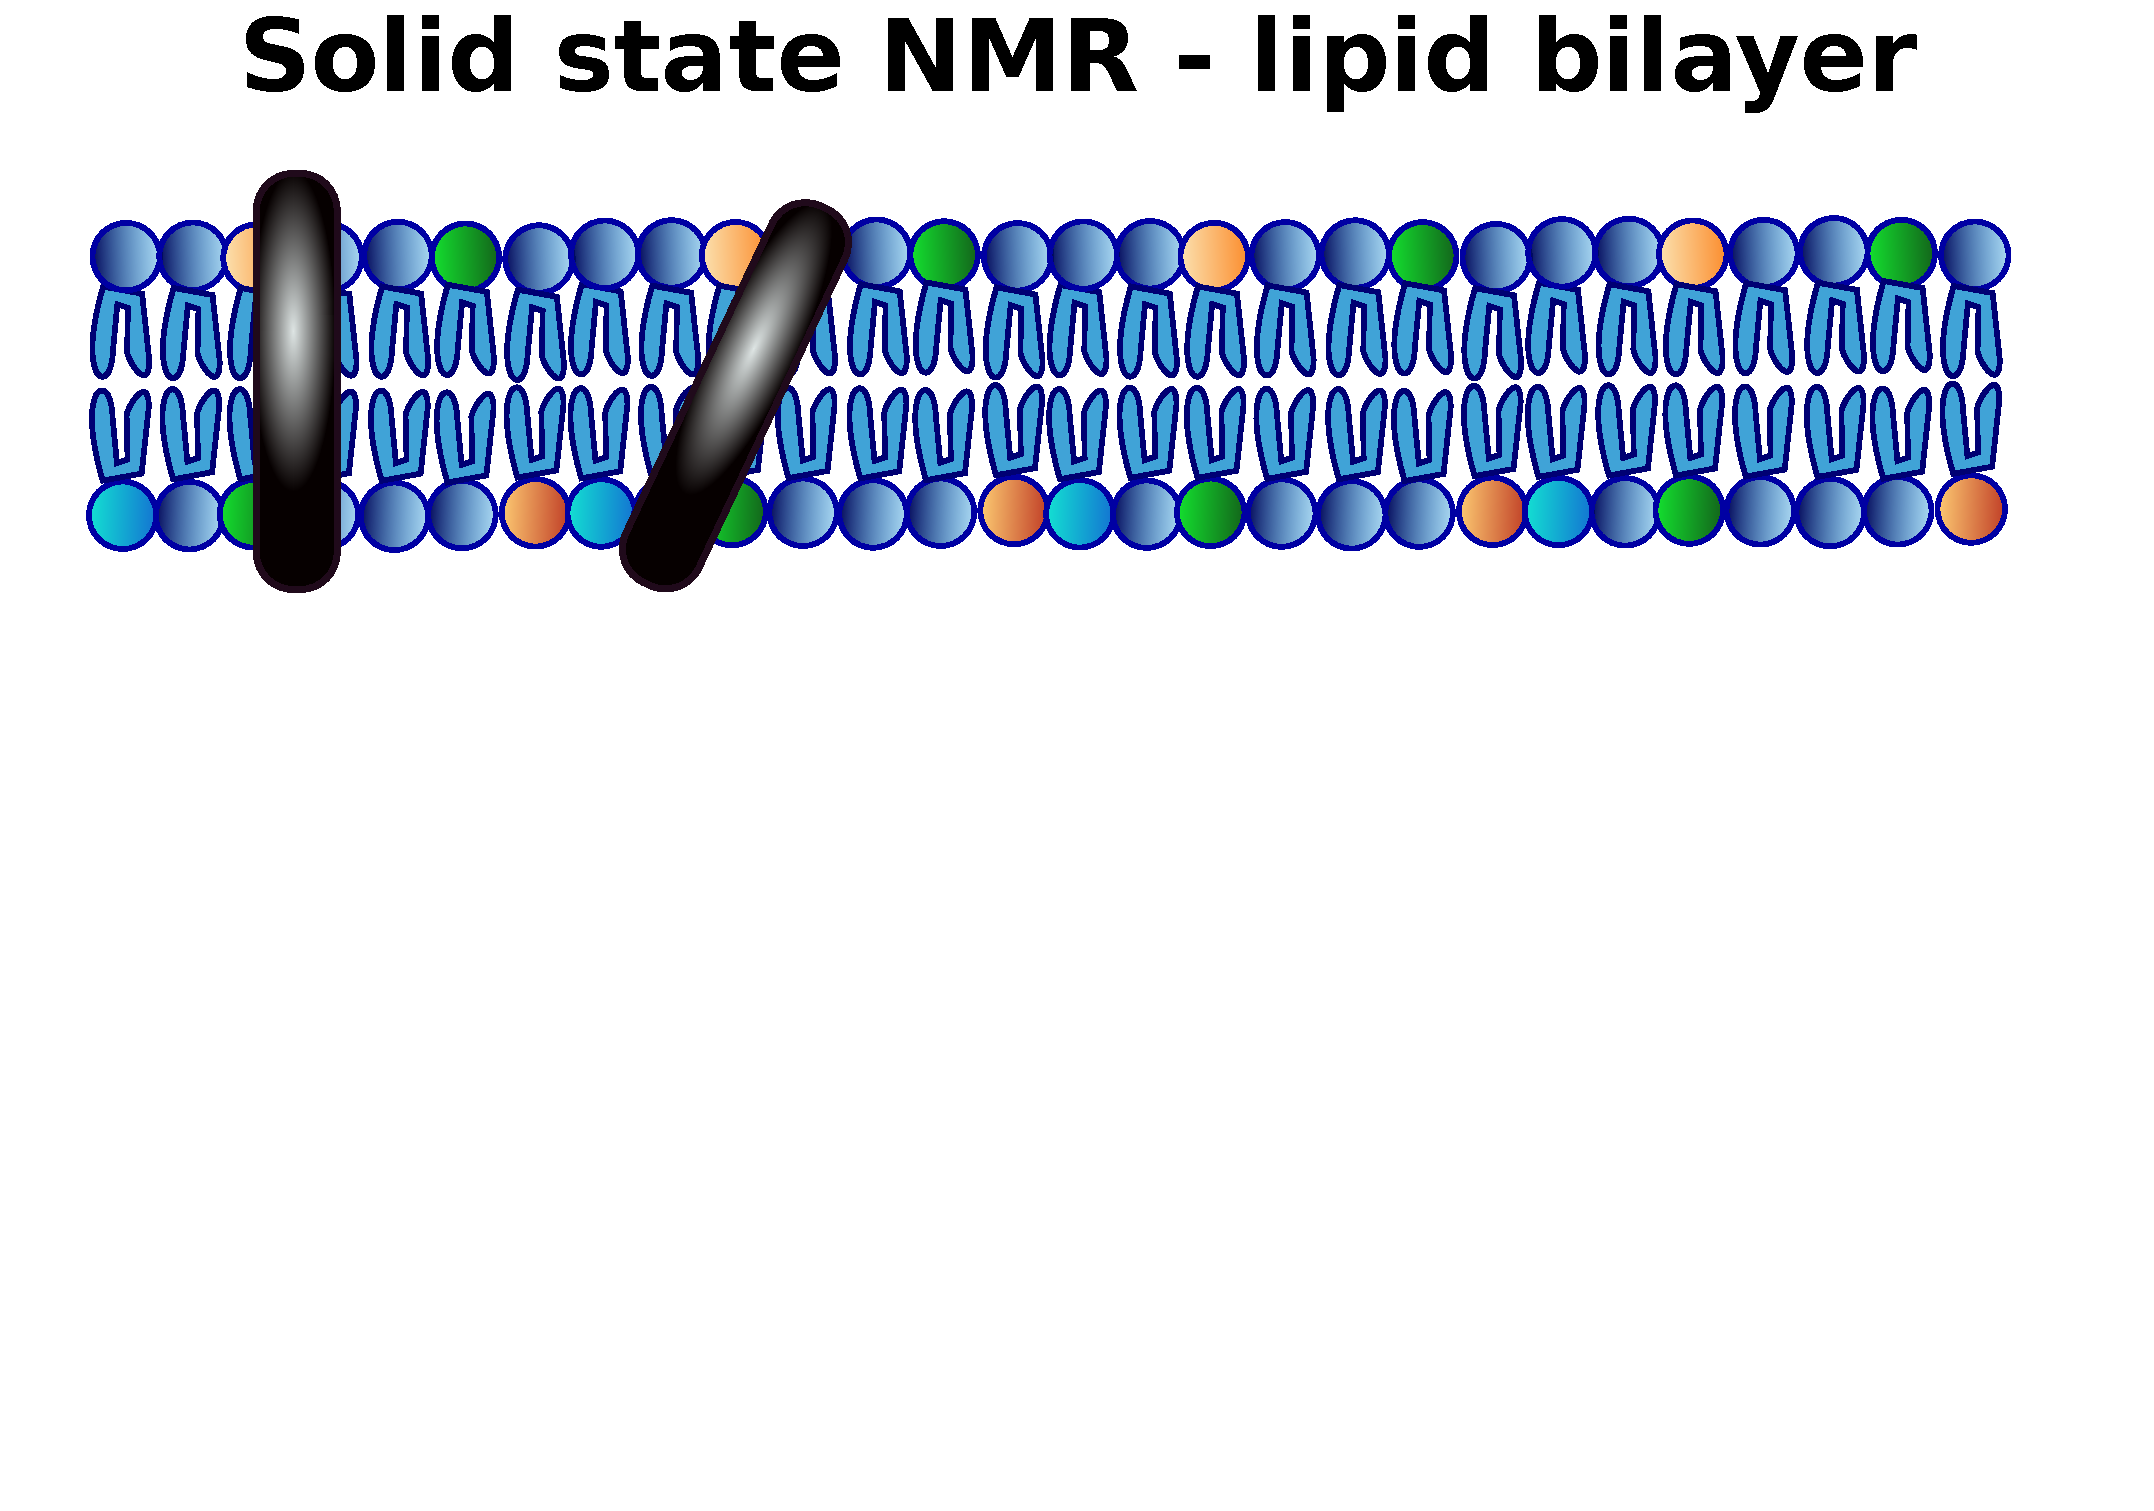
\includegraphics[height=6cm]{plots/samples7.pdf}
\end{center}
\end{frame}

\addtocounter{framenumber}{-1}
\begin{frame}
\begin{center}
\Large{\centering
\textbf{What samples can be prepared?} \\}

\vspace{0.5cm}

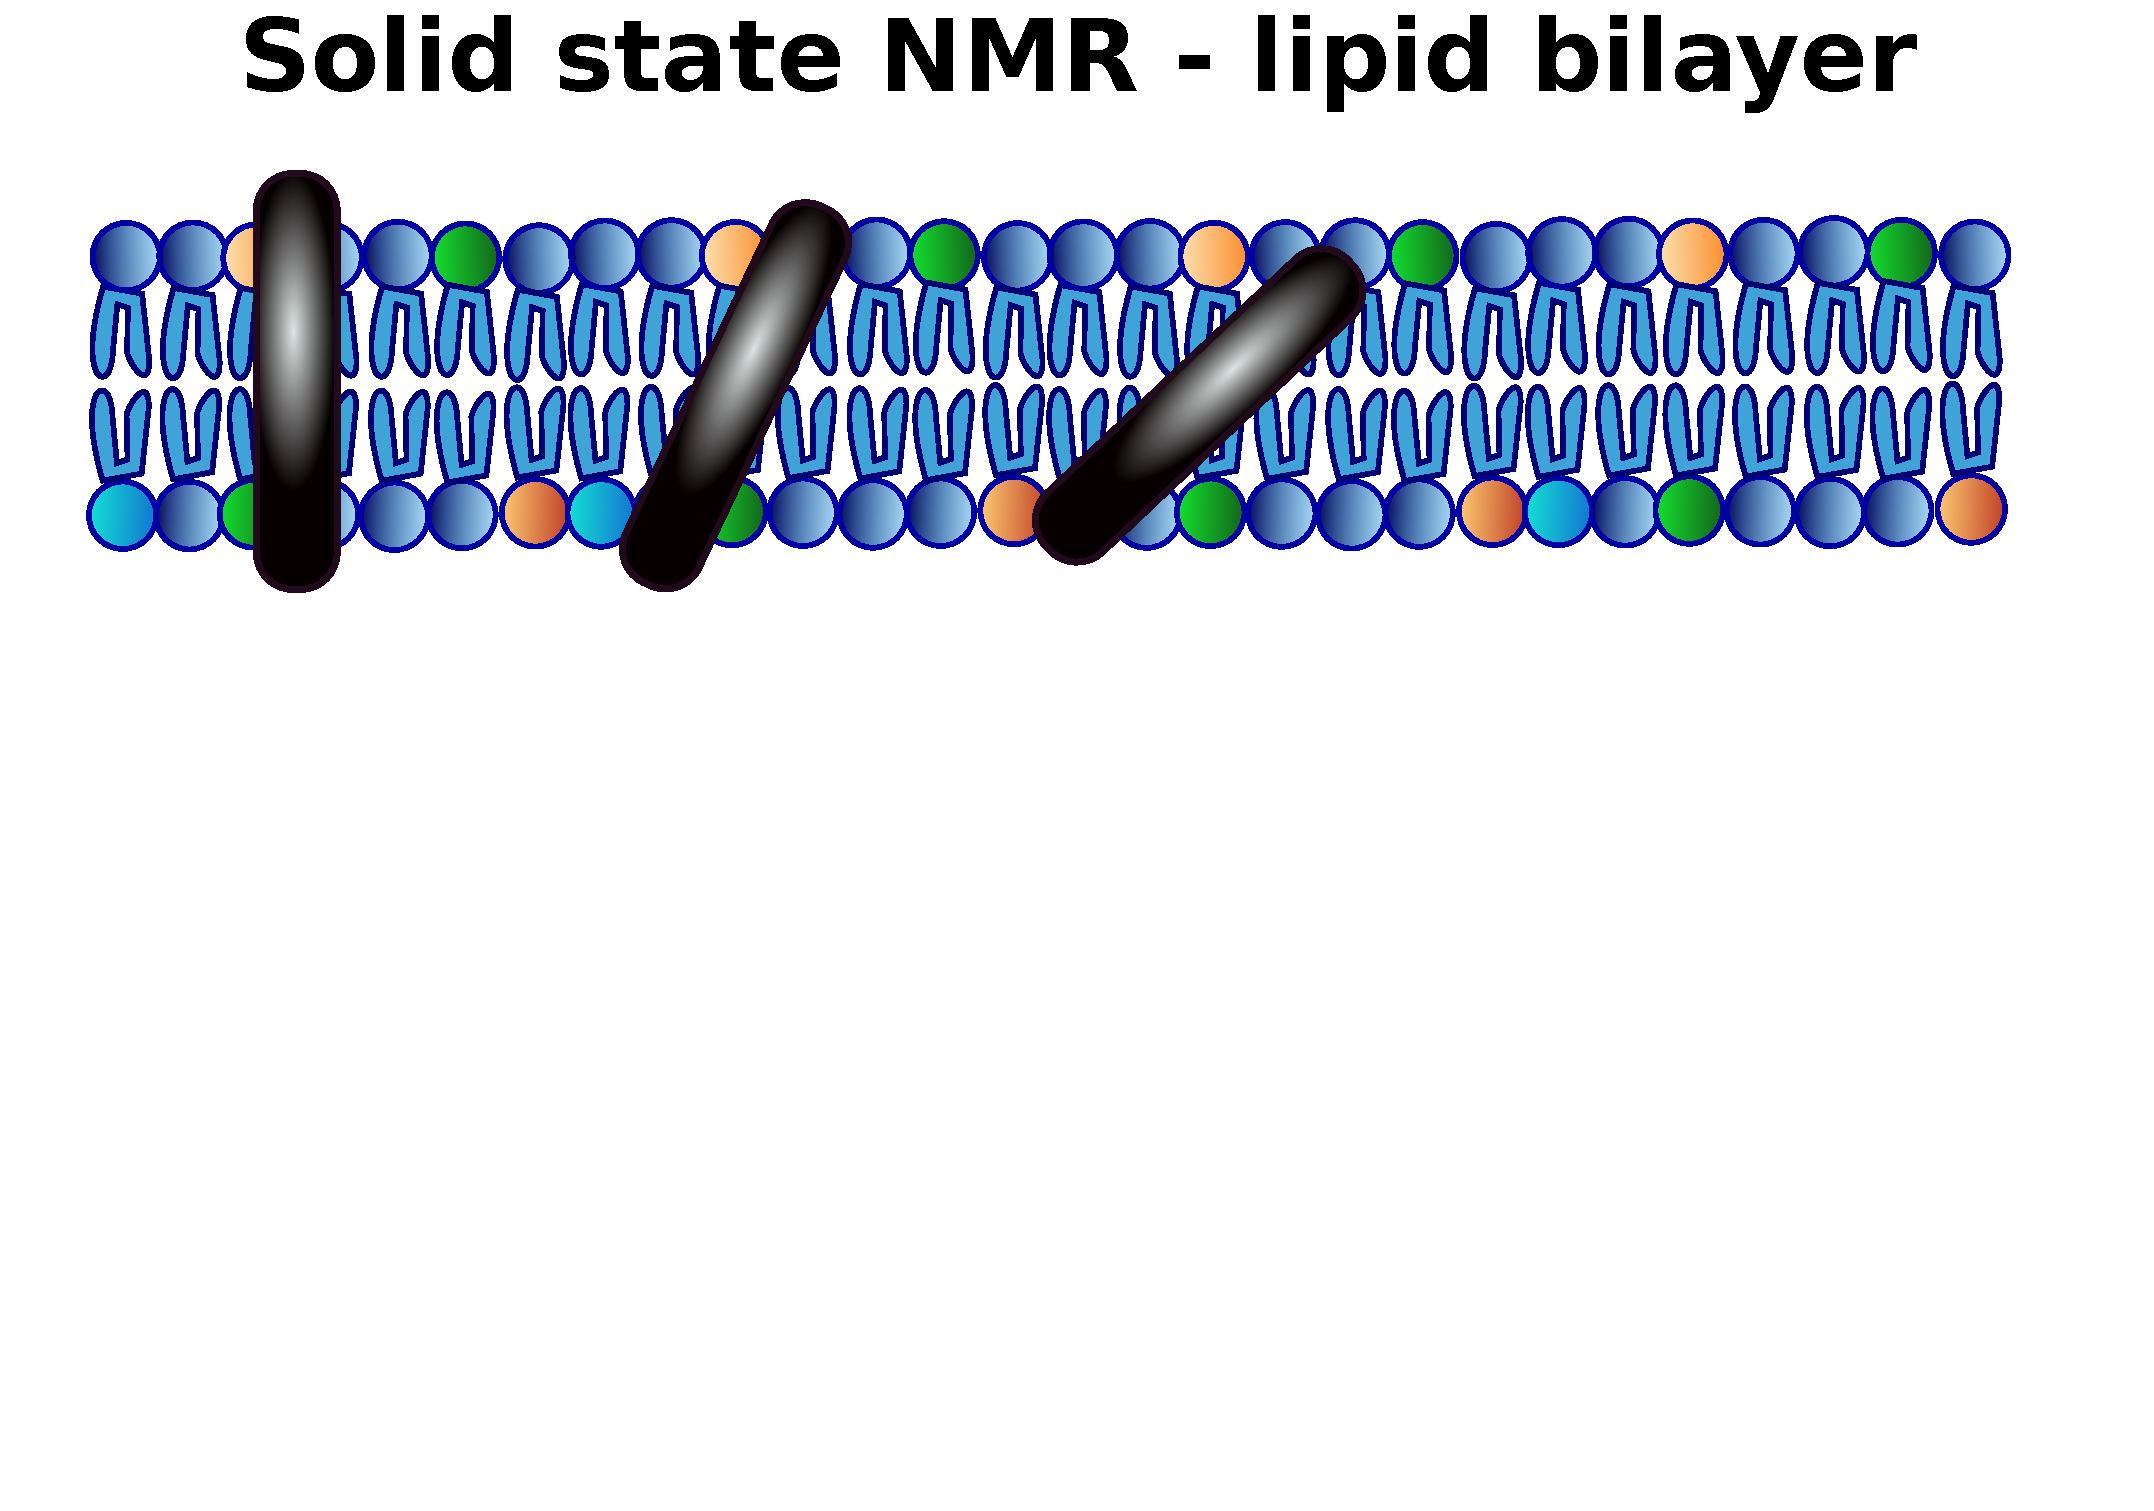
\includegraphics[height=6cm]{plots/samples6.pdf}
\end{center}
\end{frame}

\addtocounter{framenumber}{-1}
\begin{frame}
\begin{center}
\Large{\centering
\textbf{What samples can be prepared?} \\}

\vspace{0.5cm}

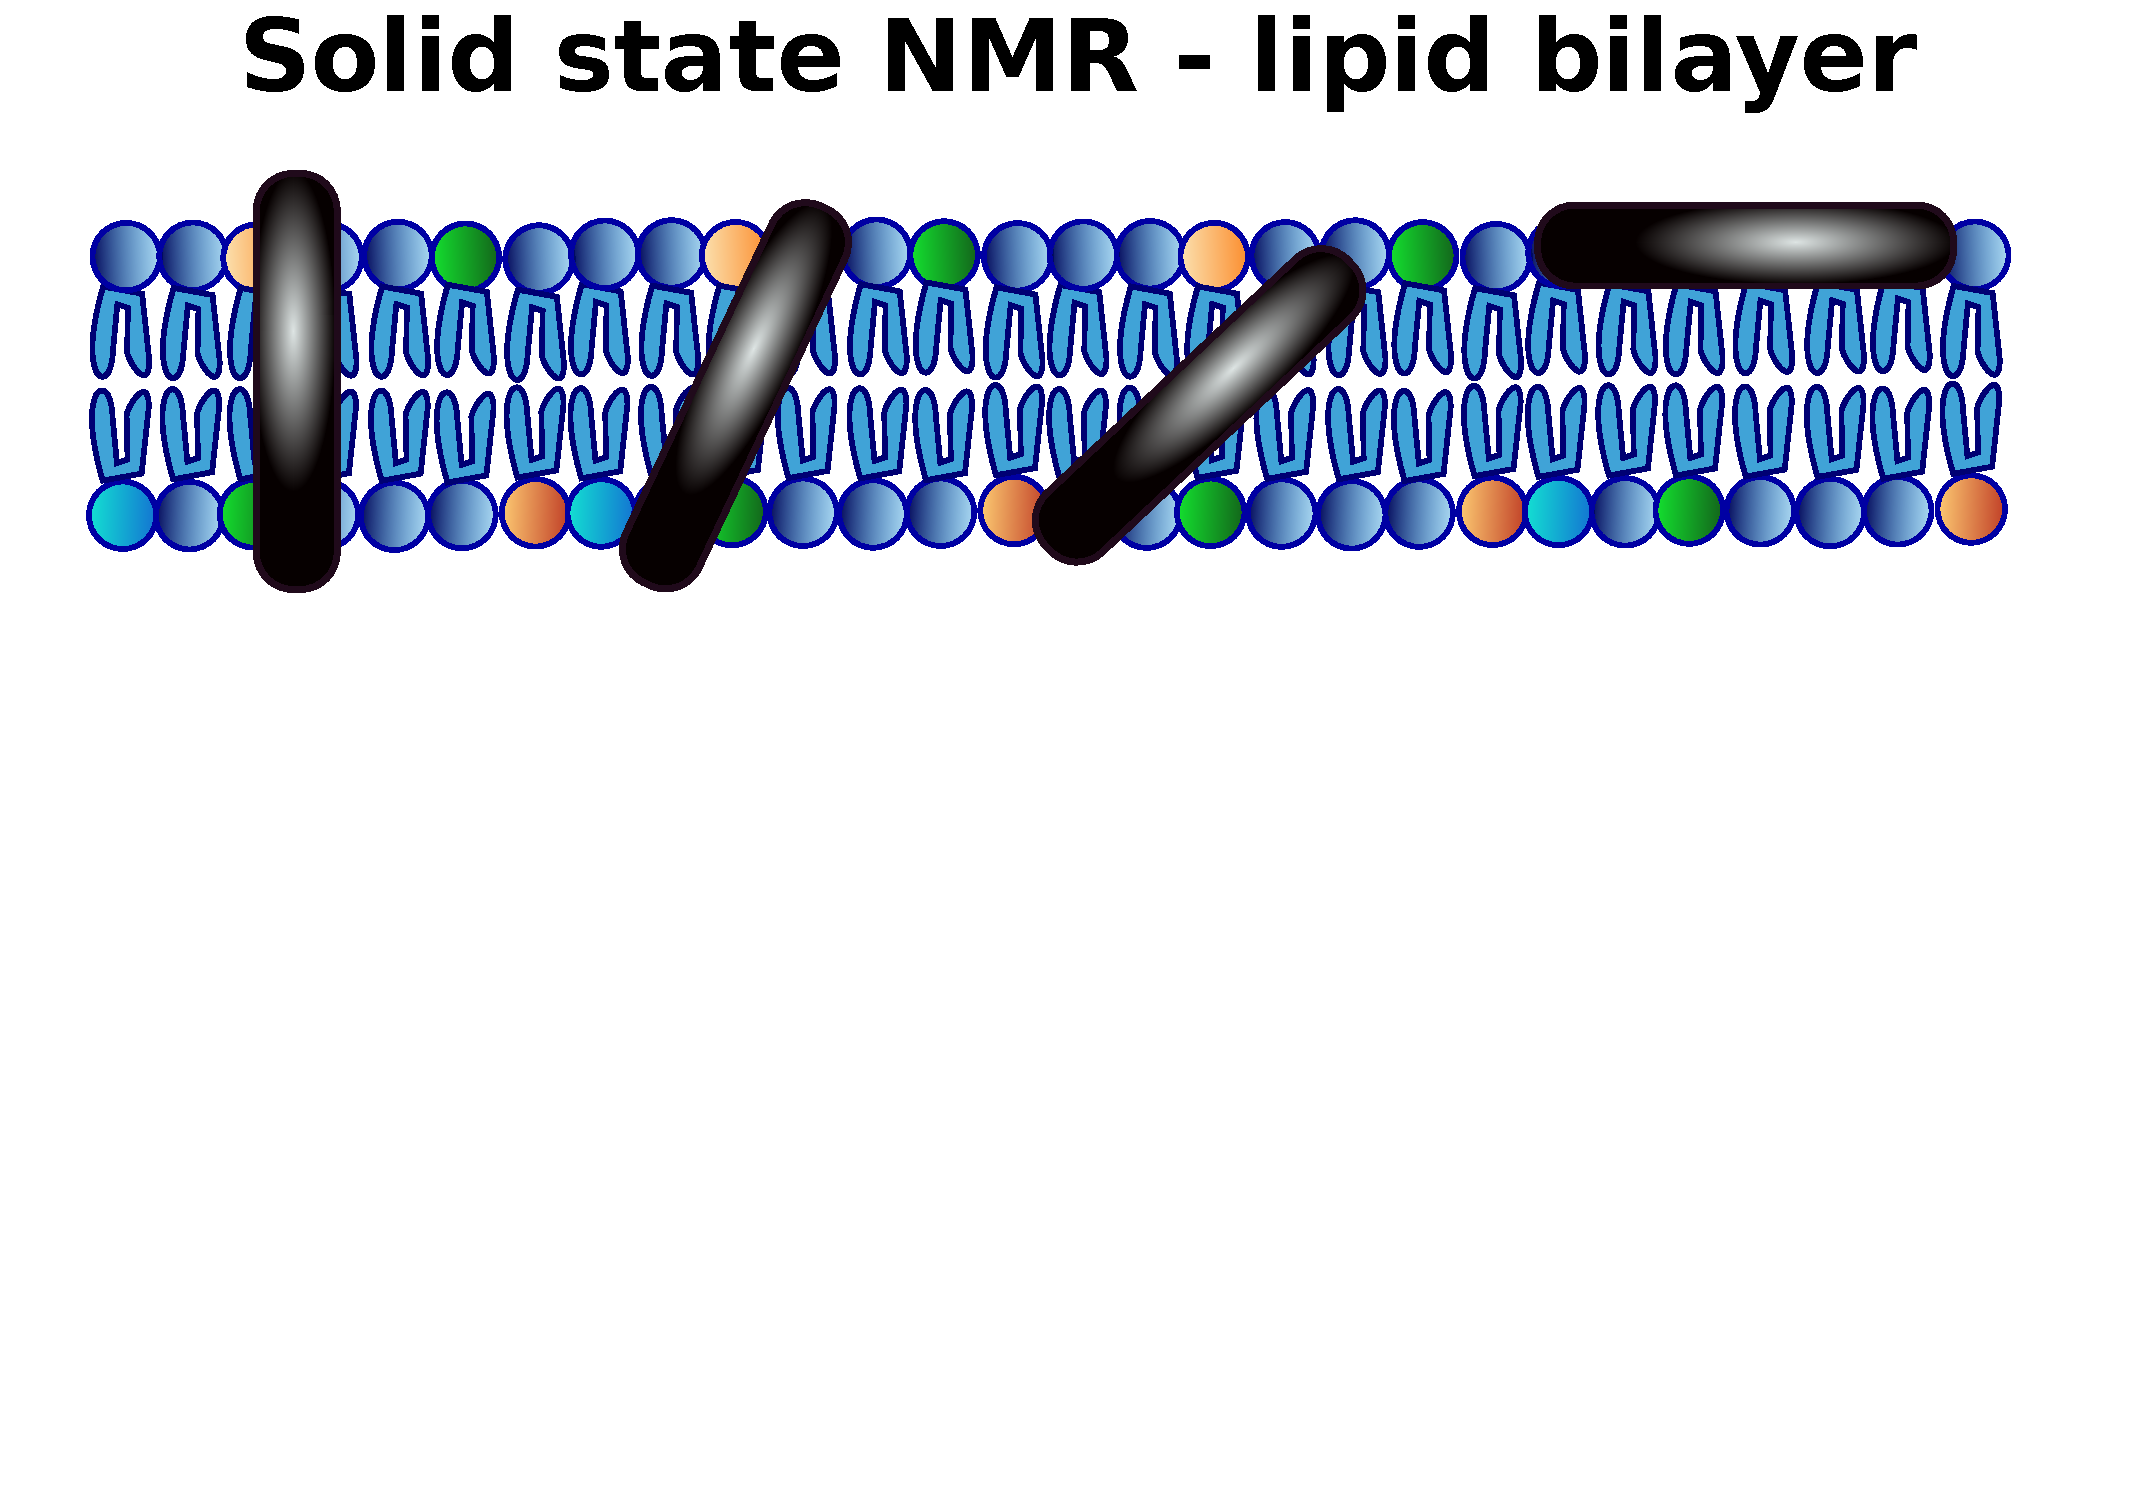
\includegraphics[height=6cm]{plots/samples5.pdf}
\end{center}
\end{frame}

\addtocounter{framenumber}{-1}
\begin{frame}
\begin{center}
\Large{\centering
\textbf{What samples can be prepared?} \\}

\vspace{0.5cm}

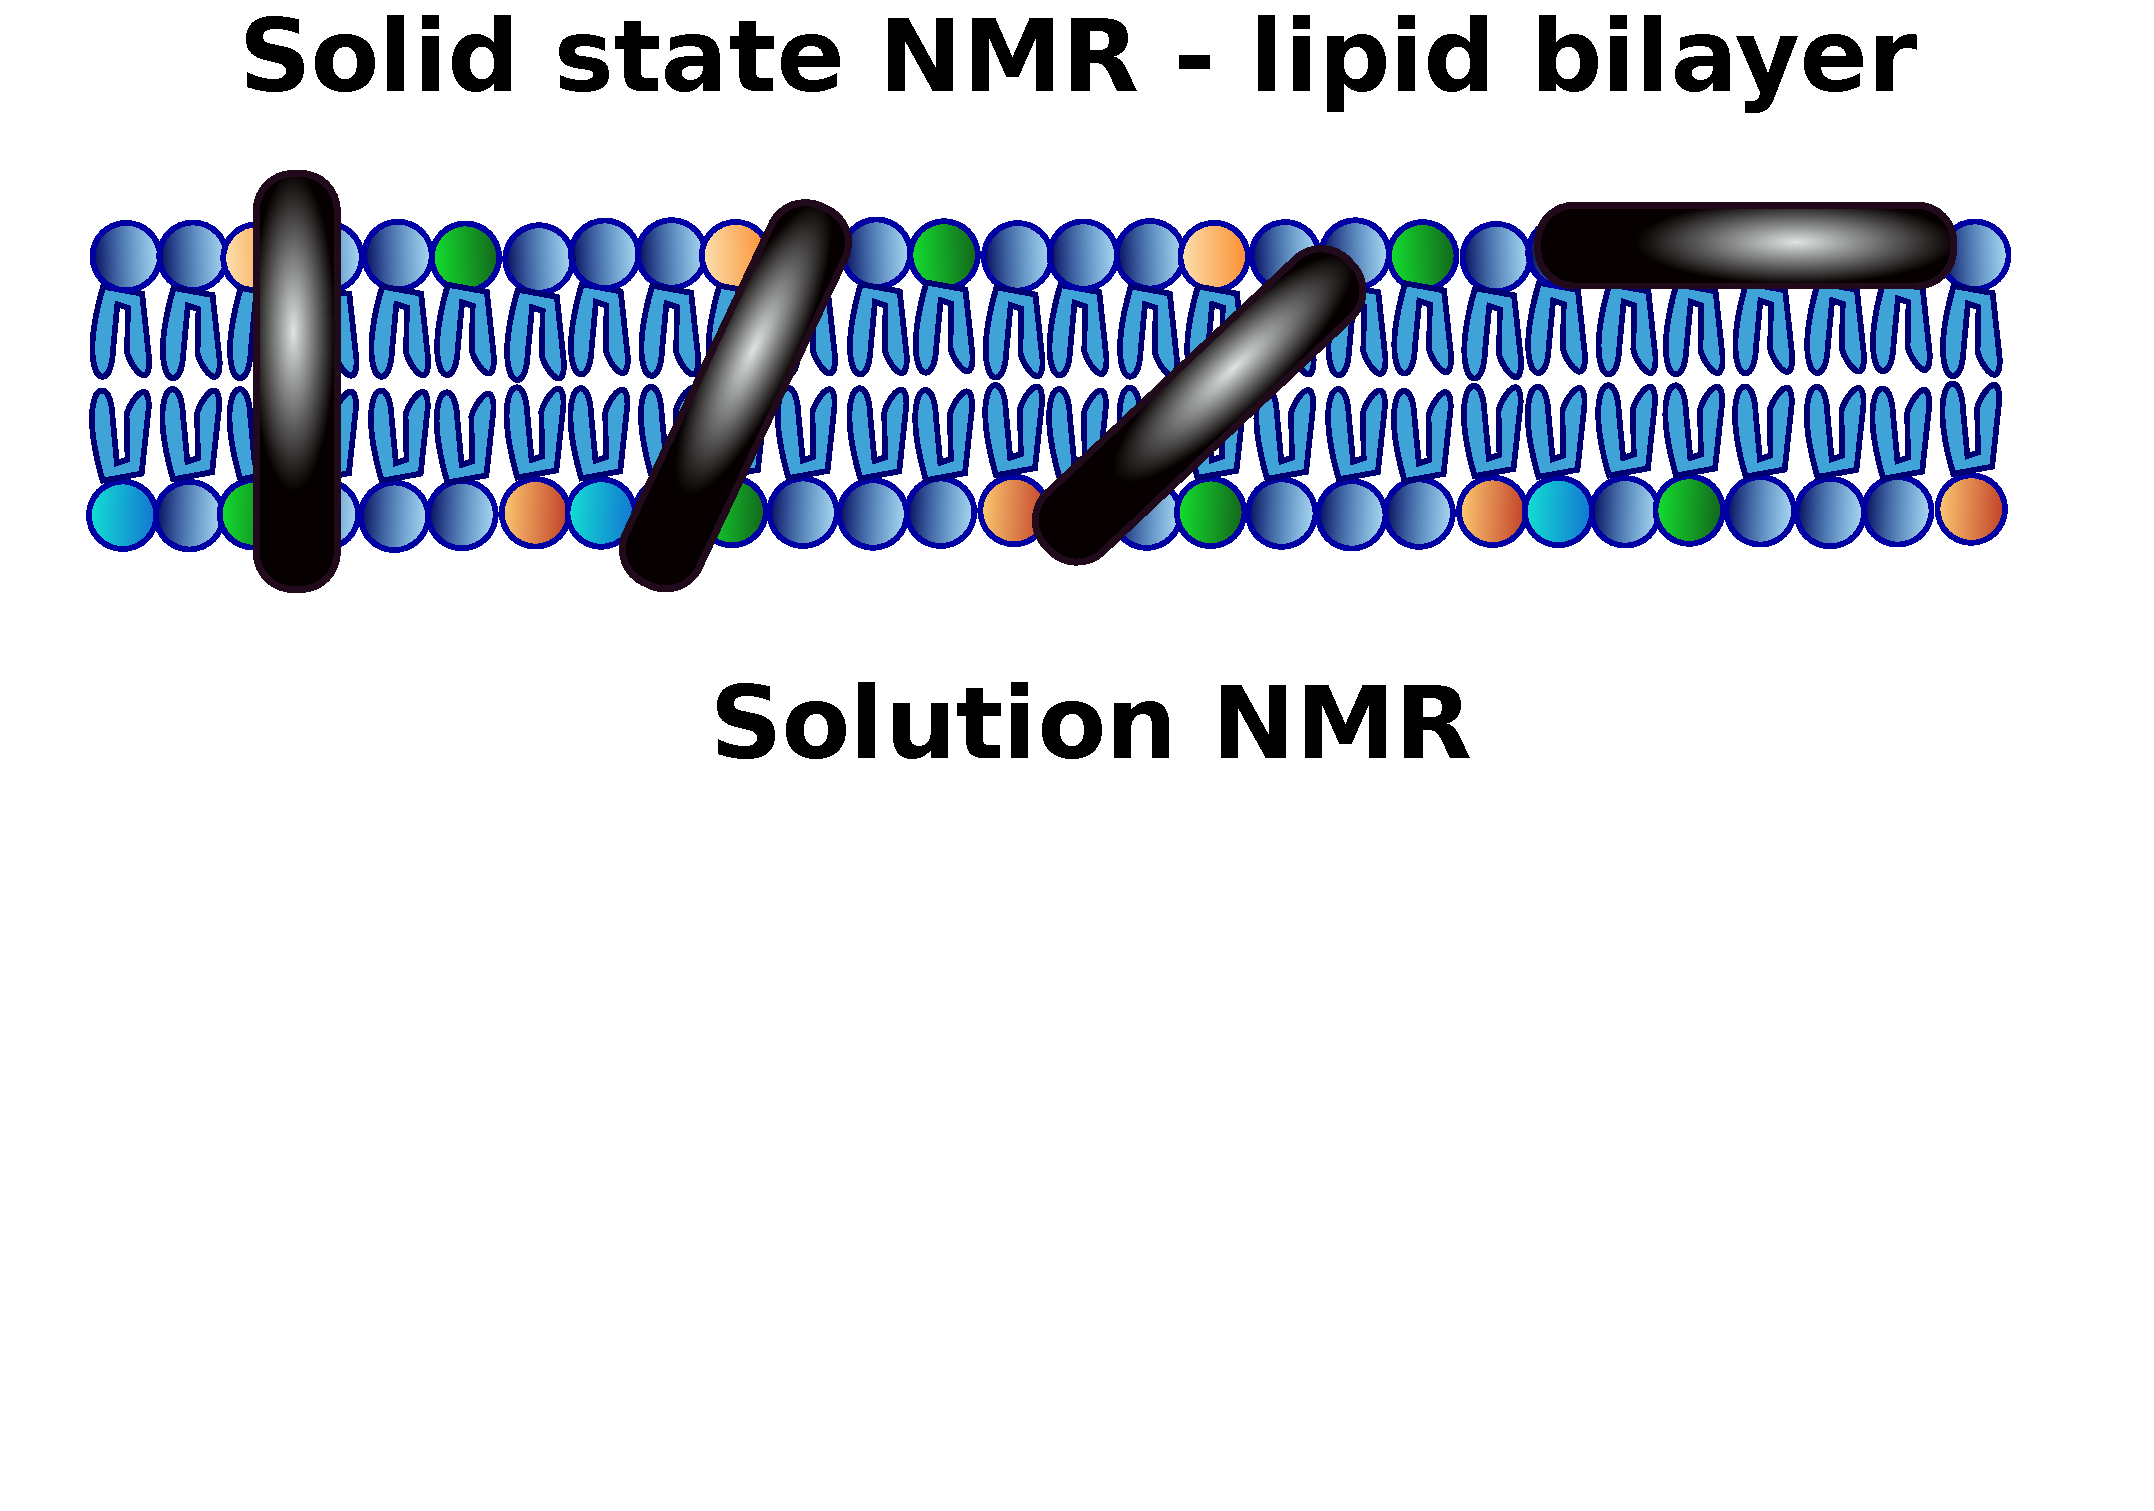
\includegraphics[height=6cm]{plots/samples4.pdf}
\end{center}
\end{frame}

\addtocounter{framenumber}{-1}
\begin{frame}
\begin{center}
\Large{\centering
\textbf{What samples can be prepared?} \\}

\vspace{0.5cm}

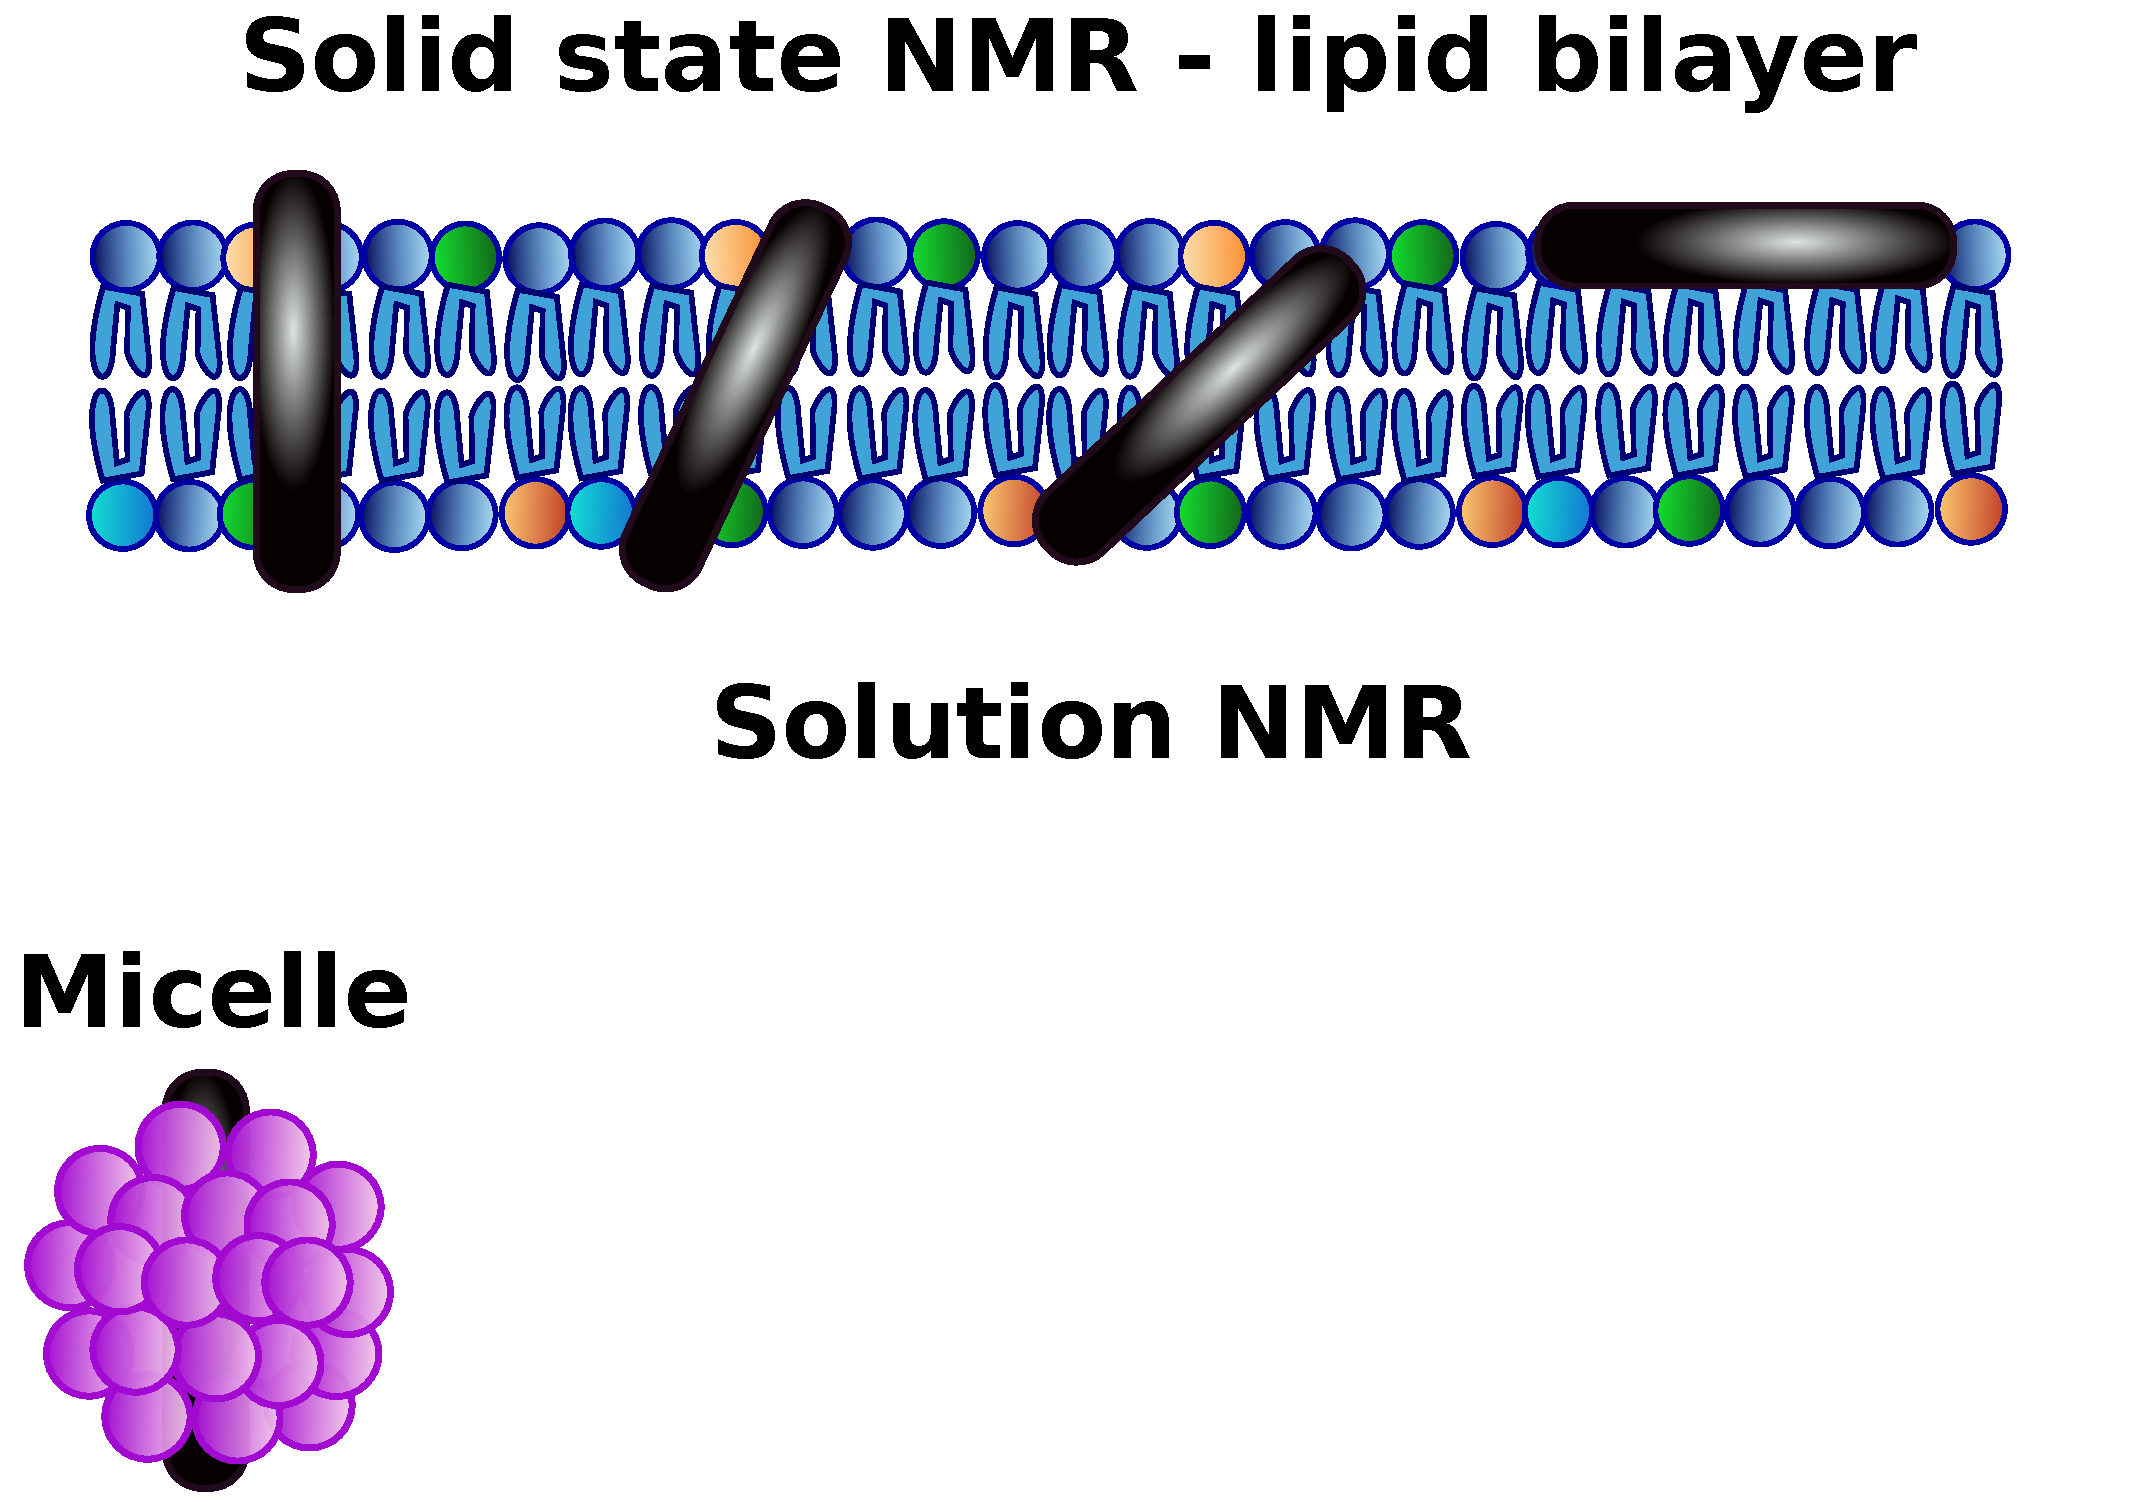
\includegraphics[height=6cm]{plots/samples3.pdf}
\end{center}
\end{frame}

\addtocounter{framenumber}{-1}
\begin{frame}
\begin{center}
\Large{\centering
\textbf{What samples can be prepared?} \\}

\vspace{0.5cm}

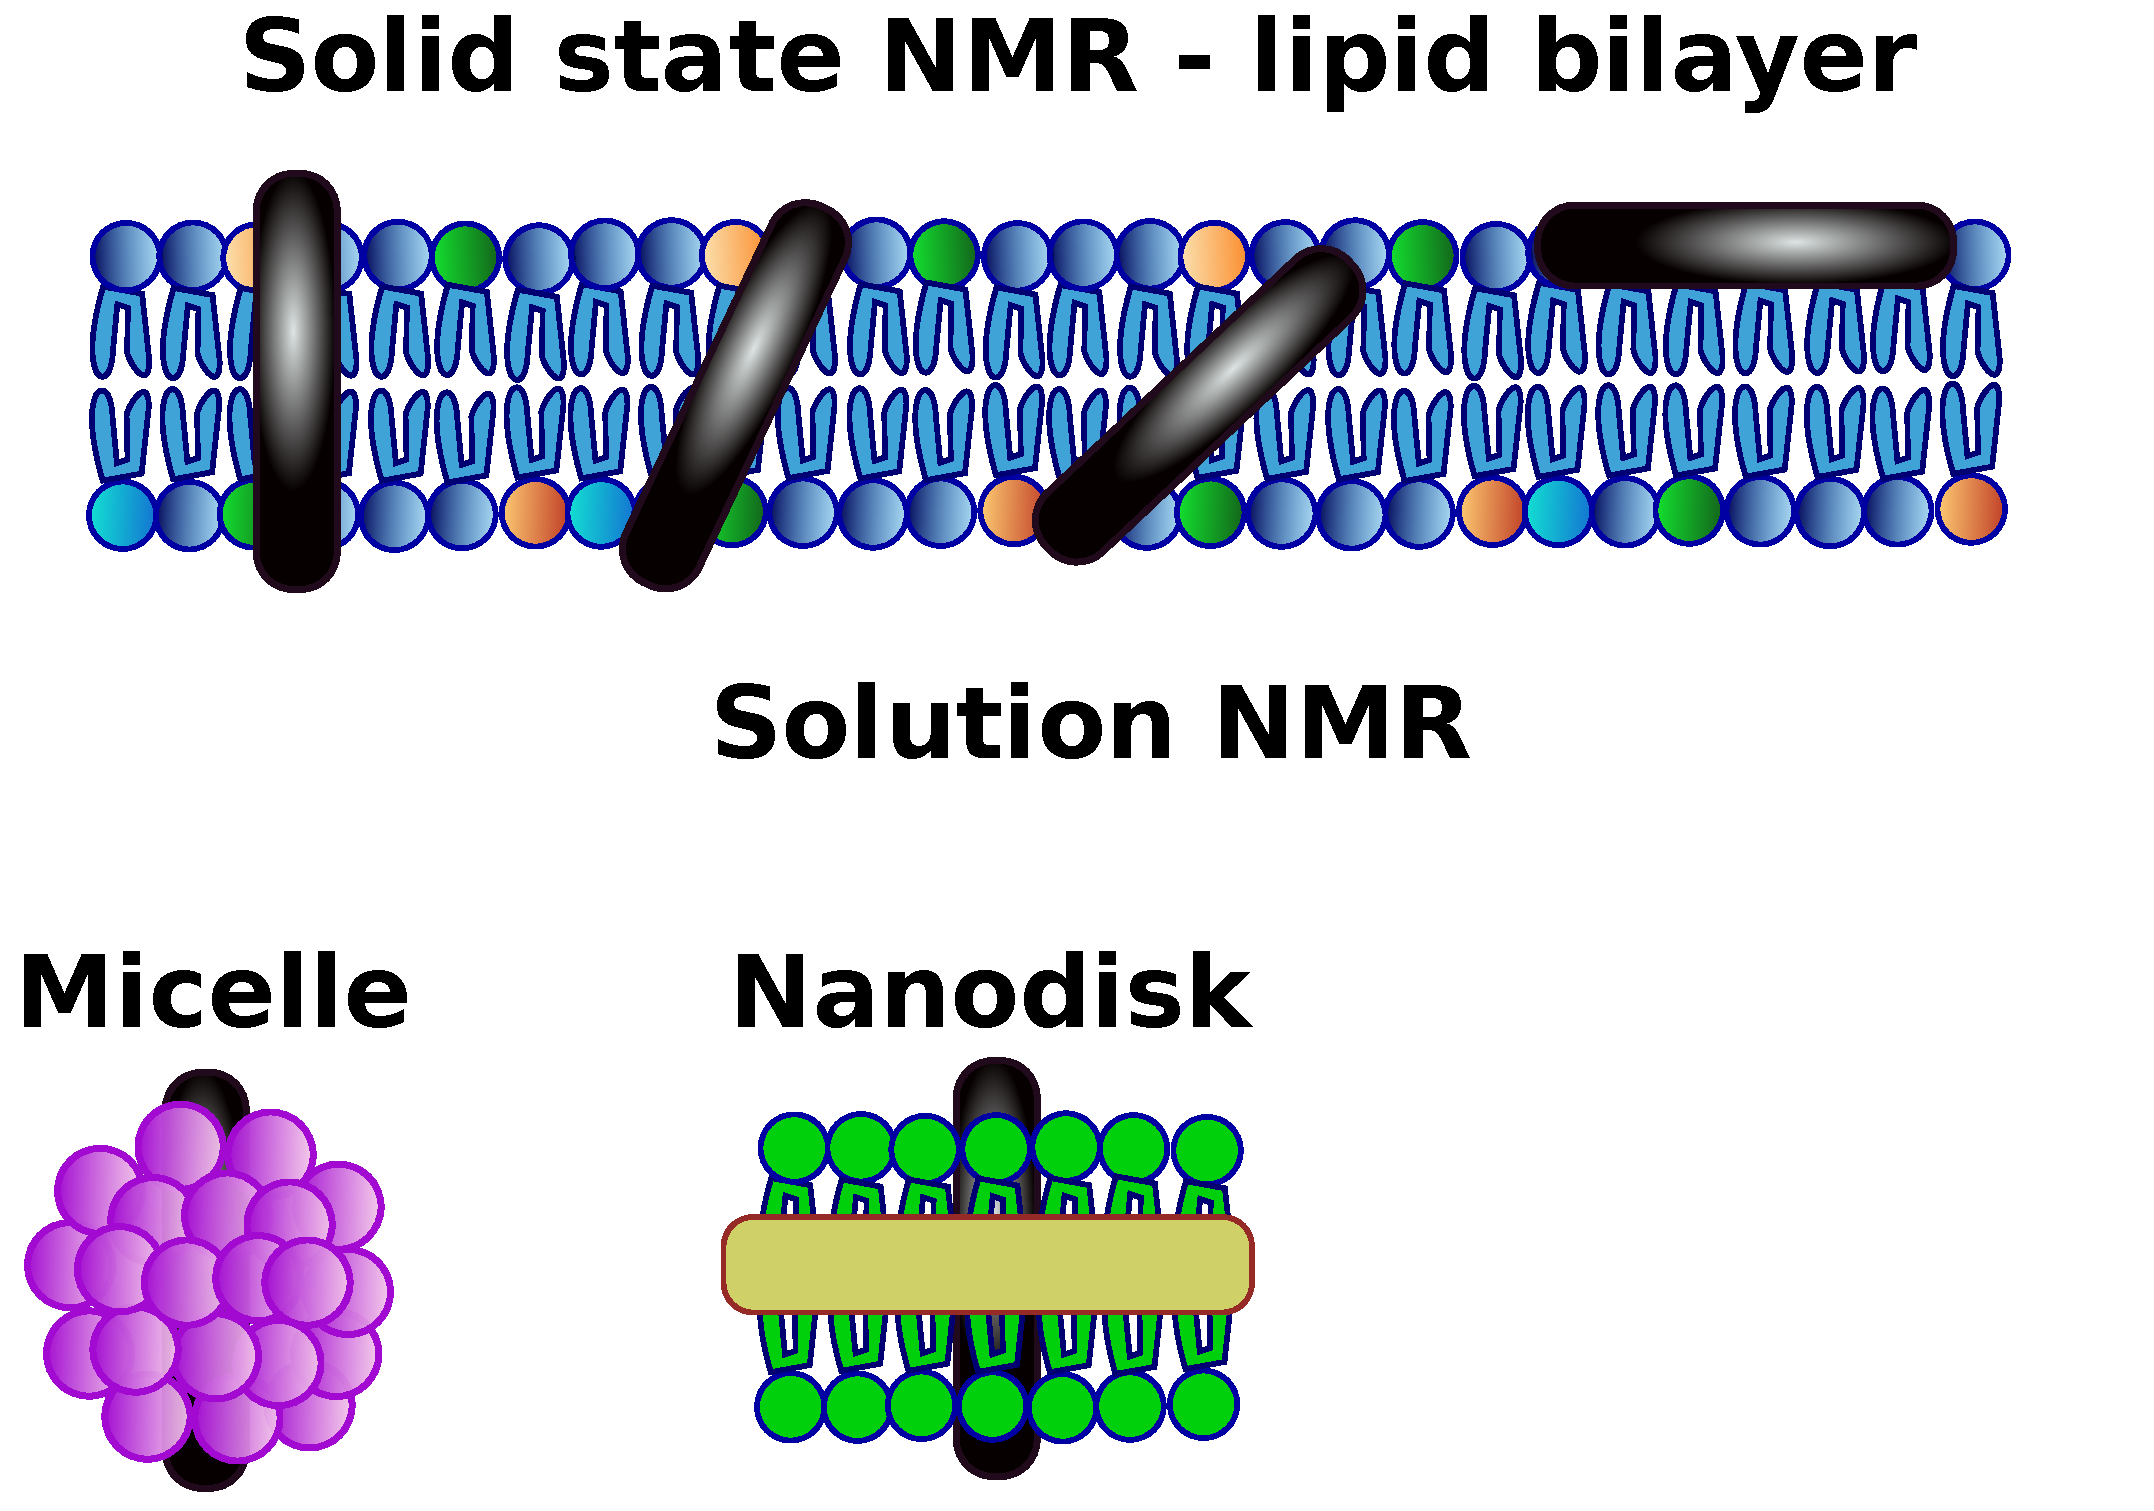
\includegraphics[height=6cm]{plots/samples2.pdf}
\end{center}
\end{frame}

\addtocounter{framenumber}{-1}
\begin{frame}
\begin{center}
\Large{\centering
\textbf{What samples can be prepared?} \\}

\vspace{0.5cm}

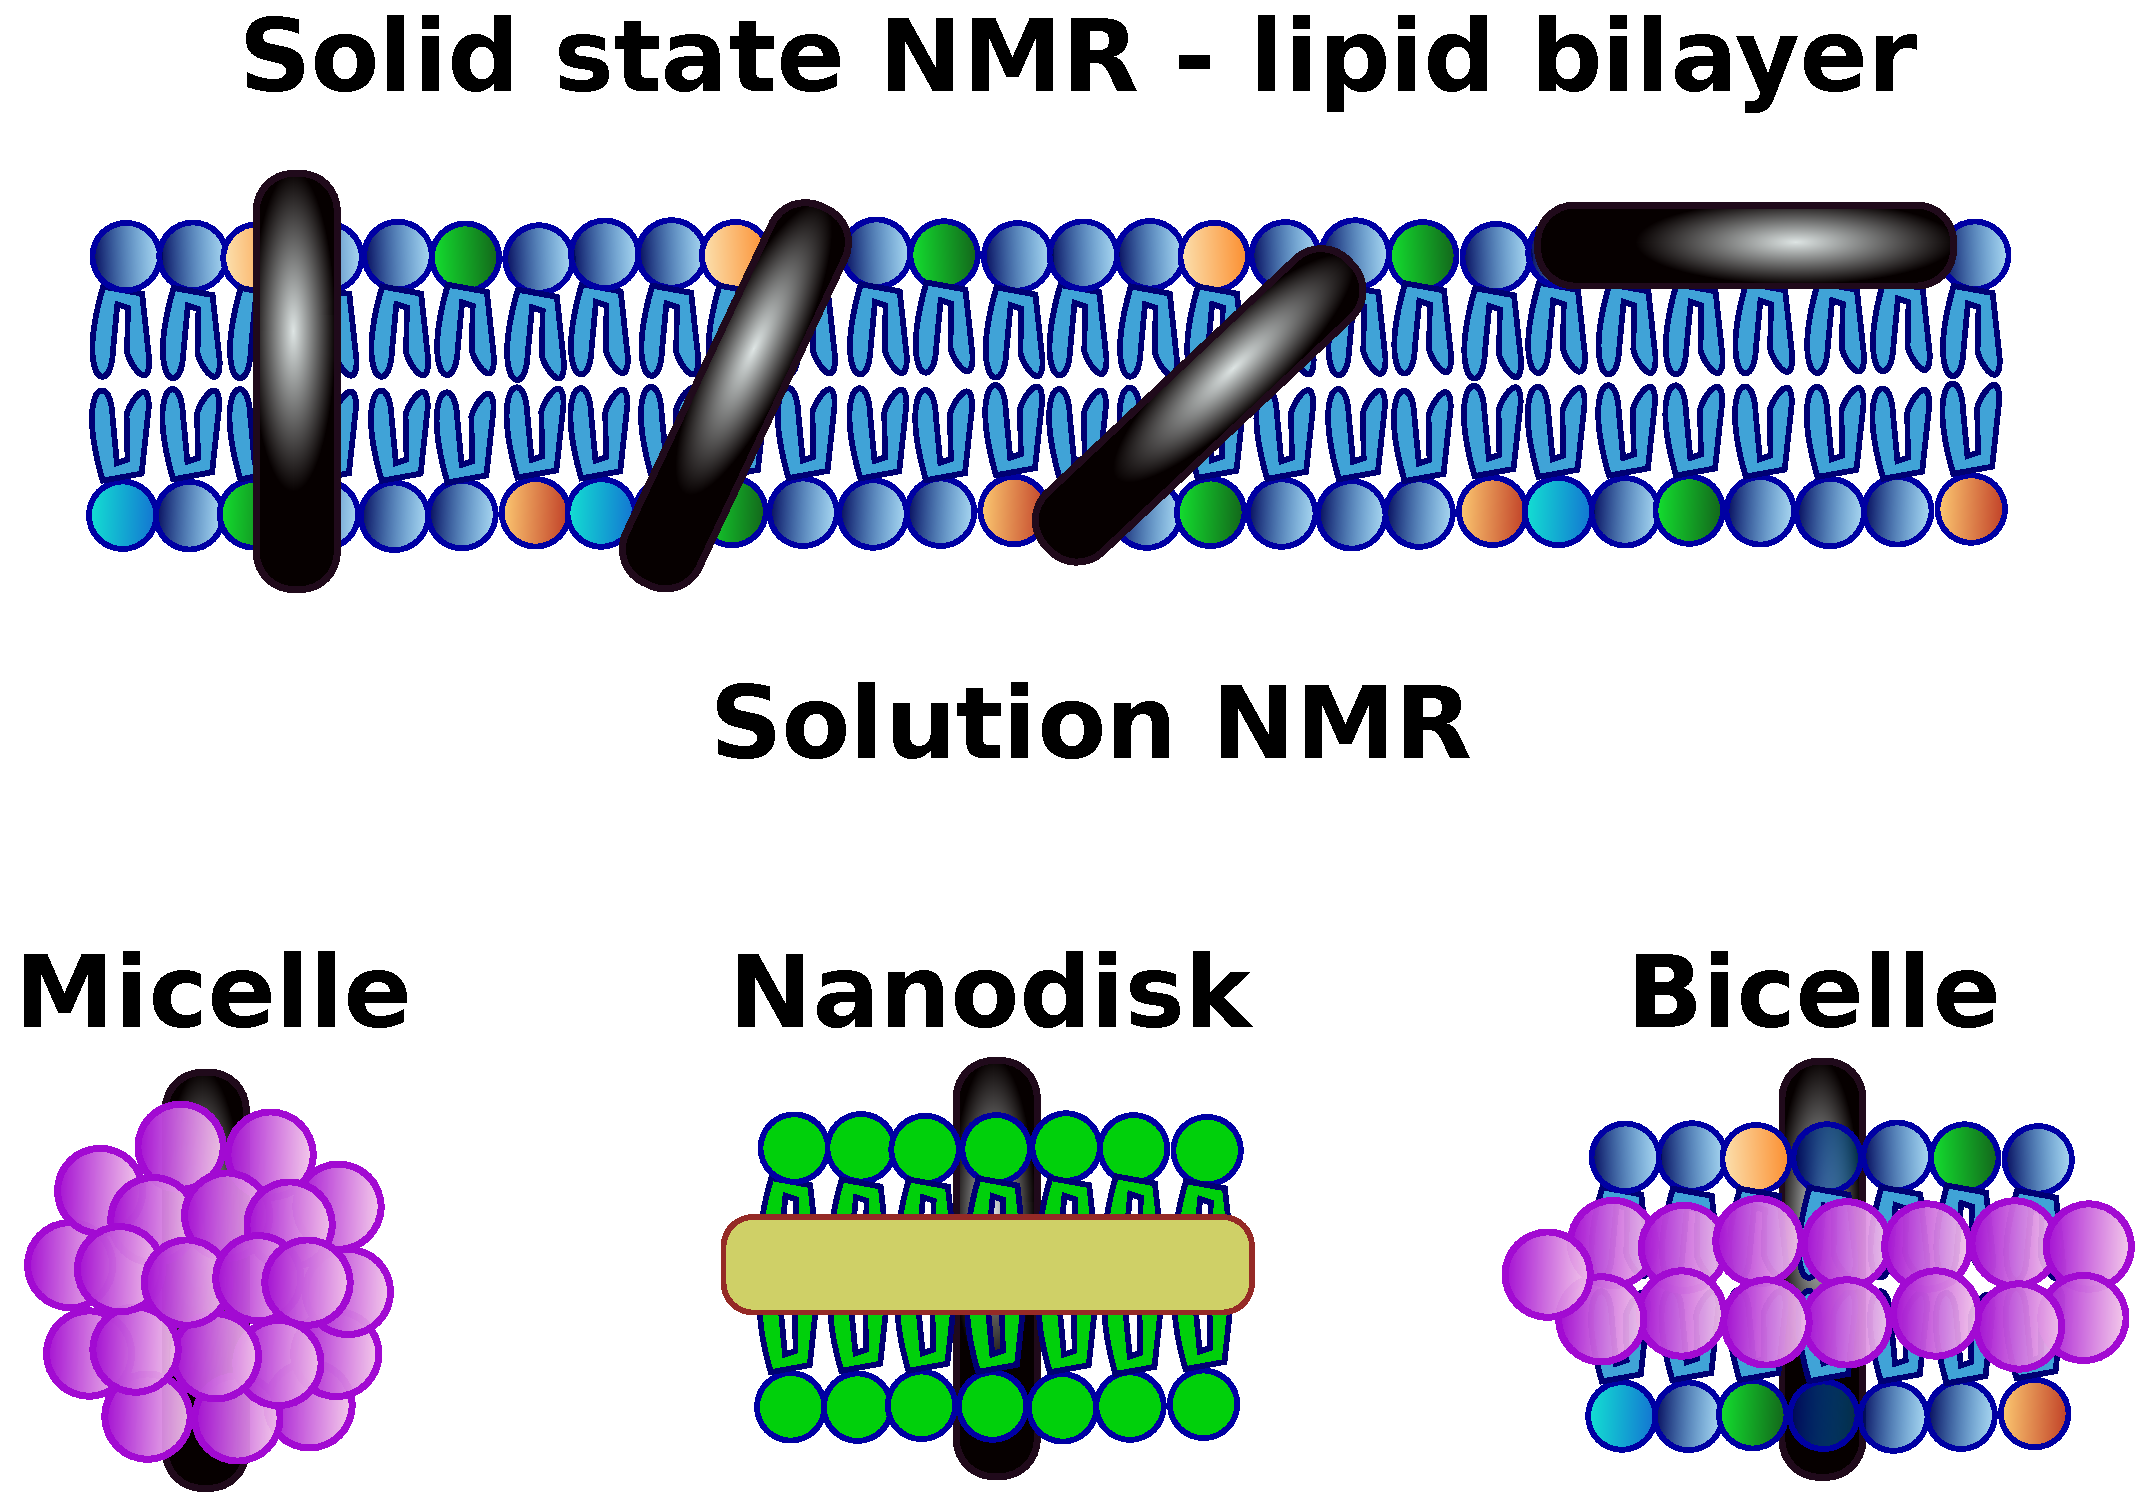
\includegraphics[height=6cm]{plots/samples1.pdf}
\end{center}
\end{frame}





\subsection{Tail Anchors}


\begin{frame}
\Large{\centering
\textbf{Case study: Tail anchored mitochondria targeted peptides} \\
to be developed
\begin{center}
 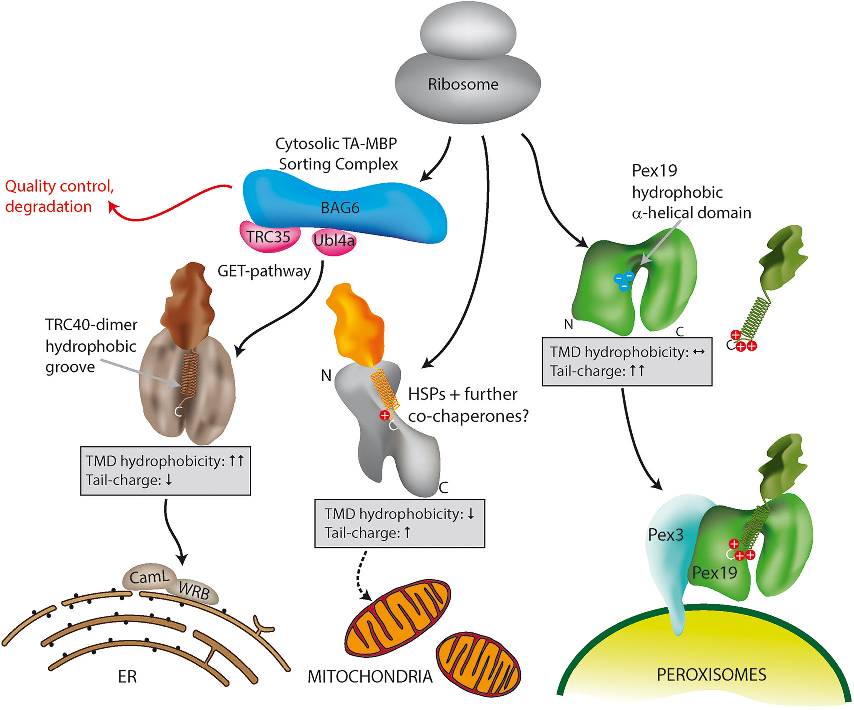
\includegraphics[height=4cm]{organels.pdf}
 %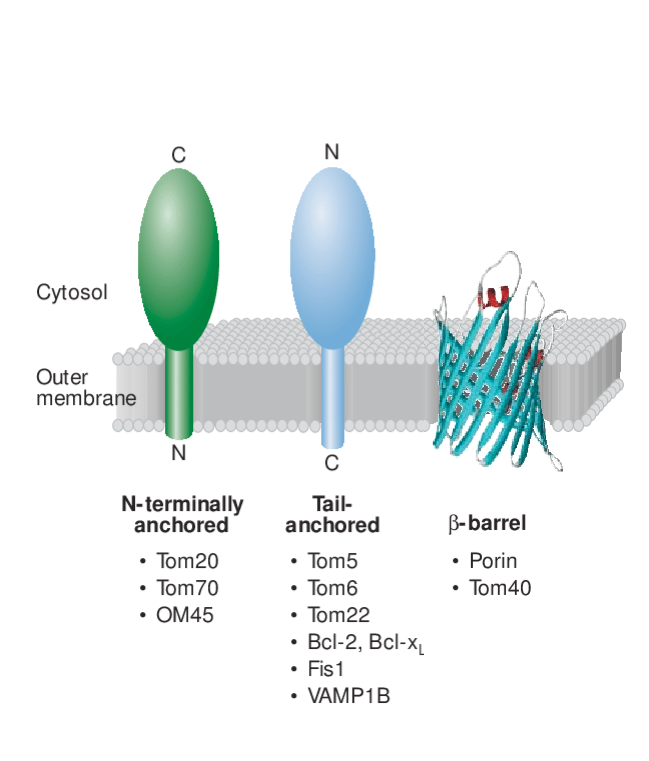
\includegraphics[height=3cm]{mitochondria2_0.png}
  % 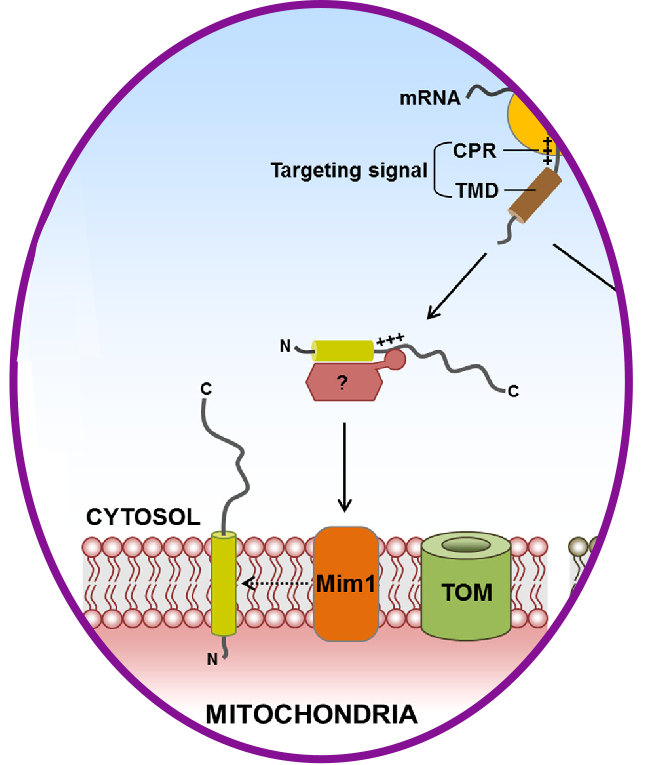
\includegraphics[height=3cm]{mitochondria2_4.png}
\end{center}
}
%{\tiny http://www.clker.com/clipart-animal-cell-3.html }
\end{frame}





\begin{frame}
\centering
\Large
Studied peptides\\

\vspace{0.3cm}

\resizebox{\textwidth}{!}{
\begin{tabular}{l l }
\hline
E.coli - ElaB & \texttt{PWQGIGVG\textcolor{red}{A}AVG\textcolor{red}{L}V\textcolor{red}{L}G\textcolor{red}{L}LL\textcolor{red}{A}RR} \\
E.coli - YqjD & \texttt{WT\textcolor{red}{G}VGIG\textcolor{red}{A}AIGVV\textcolor{red}{L}GVL\textcolor{red}{L}SRR}  \\
human - Mff & \texttt{\textcolor{red}{A}KREMVMISITV\textcolor{red}{A}FWL\textcolor{red}{L}NSW\textcolor{red}{L}WFRR}  \\
yeast - Fis1 & \texttt{\textcolor{red}{L}KGVVV\textcolor{red}{A}GGVL\textcolor{red}{A}GAVAV\textcolor{red}{A}SFF\textcolor{red}{L}RNKRR}  \\
\hline
Model - GWALP & \texttt{Ac-GG\textcolor{red}{A}LWL\textcolor{red}{A}LAL\textcolor{red}{A}LAL\textcolor{red}{A}LALWL\textcolor{red}{A}GA-NH-CH$_2$-CH$_2$OH}  \\
Model - Magainin 2 & \texttt{GIGKF\textcolor{red}{L}HS\textcolor{red}{A}KK\textcolor{red}{F}GK\textcolor{red}{A}F\textcolor{red}{V}GEIMNS } \\
\hline
\end{tabular}
}

\vspace{0.3cm}


\includegraphics[height=5cm]{tail5.pdf}
\end{frame}


\addtocounter{framenumber}{-1}
\begin{frame}
\centering
\Large
Studied peptides\\

\vspace{0.3cm}

\resizebox{\textwidth}{!}{
\begin{tabular}{l l }
\hline
E.coli - ElaB & \texttt{PWQGIGVG\textcolor{red}{A}AVG\textcolor{red}{L}V\textcolor{red}{L}G\textcolor{red}{L}LL\textcolor{red}{A}RR} \\
E.coli - YqjD & \texttt{WT\textcolor{red}{G}VGIG\textcolor{red}{A}AIGVV\textcolor{red}{L}GVL\textcolor{red}{L}SRR}  \\
human - Mff & \texttt{\textcolor{red}{A}KREMVMISITV\textcolor{red}{A}FWL\textcolor{red}{L}NSW\textcolor{red}{L}WFRR}  \\
yeast - Fis1 & \texttt{\textcolor{red}{L}KGVVV\textcolor{red}{A}GGVL\textcolor{red}{A}GAVAV\textcolor{red}{A}SFF\textcolor{red}{L}RNKRR}  \\
\hline
Model - GWALP & \texttt{Ac-GG\textcolor{red}{A}LWL\textcolor{red}{A}LAL\textcolor{red}{A}LAL\textcolor{red}{A}LALWL\textcolor{red}{A}GA-NH-CH$_2$-CH$_2$OH}  \\
Model - Magainin 2 & \texttt{GIGKF\textcolor{red}{L}HS\textcolor{red}{A}KK\textcolor{red}{F}GK\textcolor{red}{A}F\textcolor{red}{V}GEIMNS } \\
\hline
\end{tabular}
}

\vspace{0.3cm}

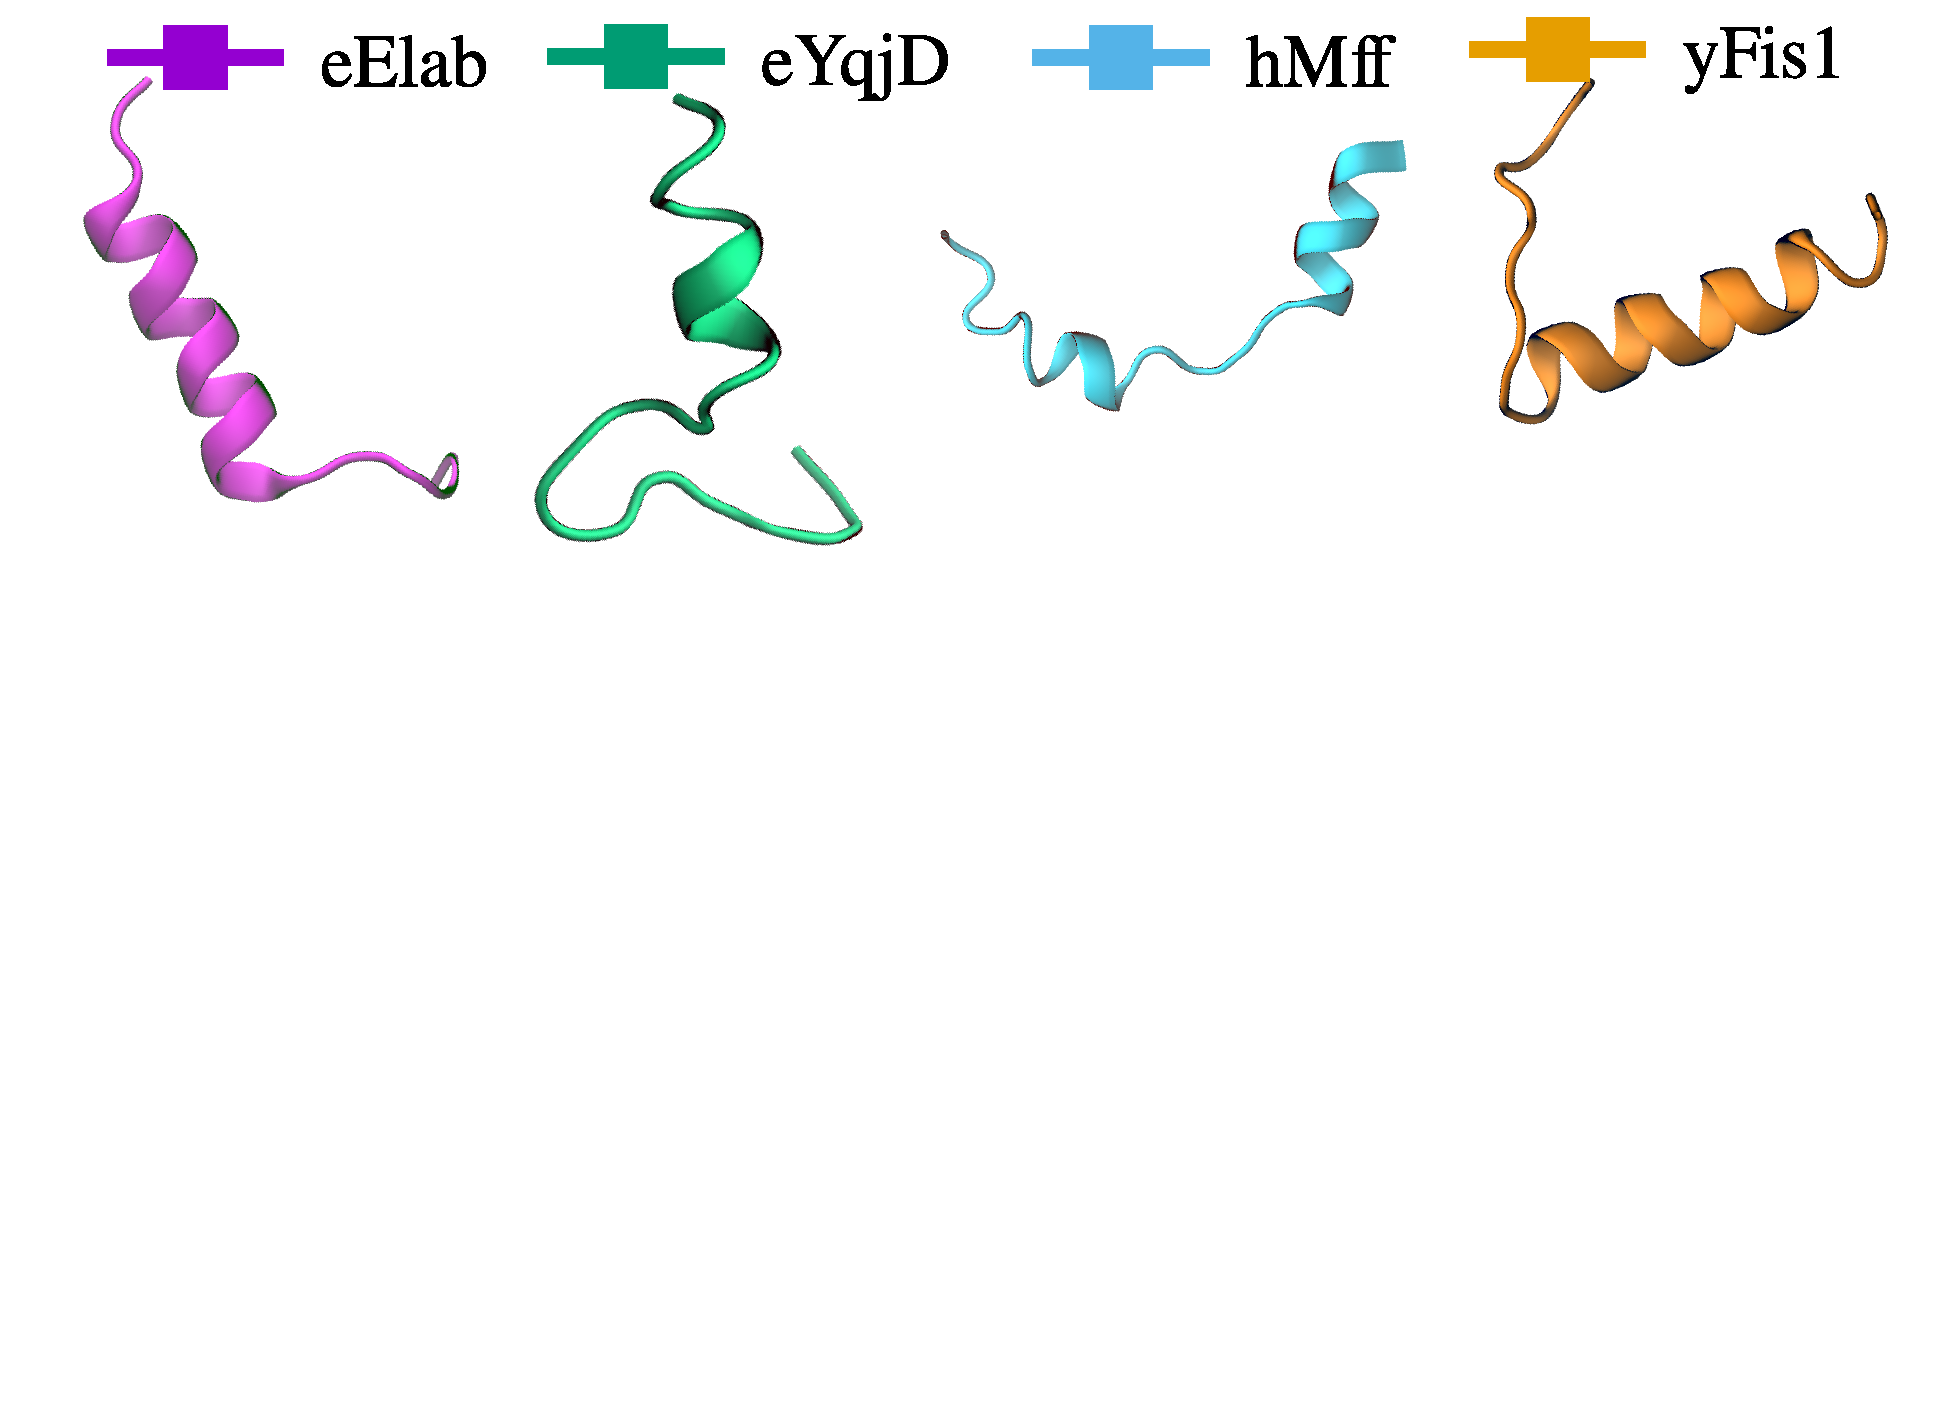
\includegraphics[height=5cm]{tail4.pdf}
\end{frame}



\addtocounter{framenumber}{-1}
\begin{frame}
\centering
\Large
Studied peptides\\

\vspace{0.3cm}

\resizebox{\textwidth}{!}{
\begin{tabular}{l l }
\hline
E.coli - ElaB & \texttt{PWQGIGVG\textcolor{red}{A}AVG\textcolor{red}{L}V\textcolor{red}{L}G\textcolor{red}{L}LL\textcolor{red}{A}RR} \\
E.coli - YqjD & \texttt{WT\textcolor{red}{G}VGIG\textcolor{red}{A}AIGVV\textcolor{red}{L}GVL\textcolor{red}{L}SRR}  \\
human - Mff & \texttt{\textcolor{red}{A}KREMVMISITV\textcolor{red}{A}FWL\textcolor{red}{L}NSW\textcolor{red}{L}WFRR}  \\
yeast - Fis1 & \texttt{\textcolor{red}{L}KGVVV\textcolor{red}{A}GGVL\textcolor{red}{A}GAVAV\textcolor{red}{A}SFF\textcolor{red}{L}RNKRR}  \\
\hline
Model - GWALP & \texttt{Ac-GG\textcolor{red}{A}LWL\textcolor{red}{A}LAL\textcolor{red}{A}LAL\textcolor{red}{A}LALWL\textcolor{red}{A}GA-NH-CH$_2$-CH$_2$OH}  \\
Model - Magainin 2 & \texttt{GIGKF\textcolor{red}{L}HS\textcolor{red}{A}KK\textcolor{red}{F}GK\textcolor{red}{A}F\textcolor{red}{V}GEIMNS } \\
\hline
\end{tabular}
}

\vspace{0.3cm}

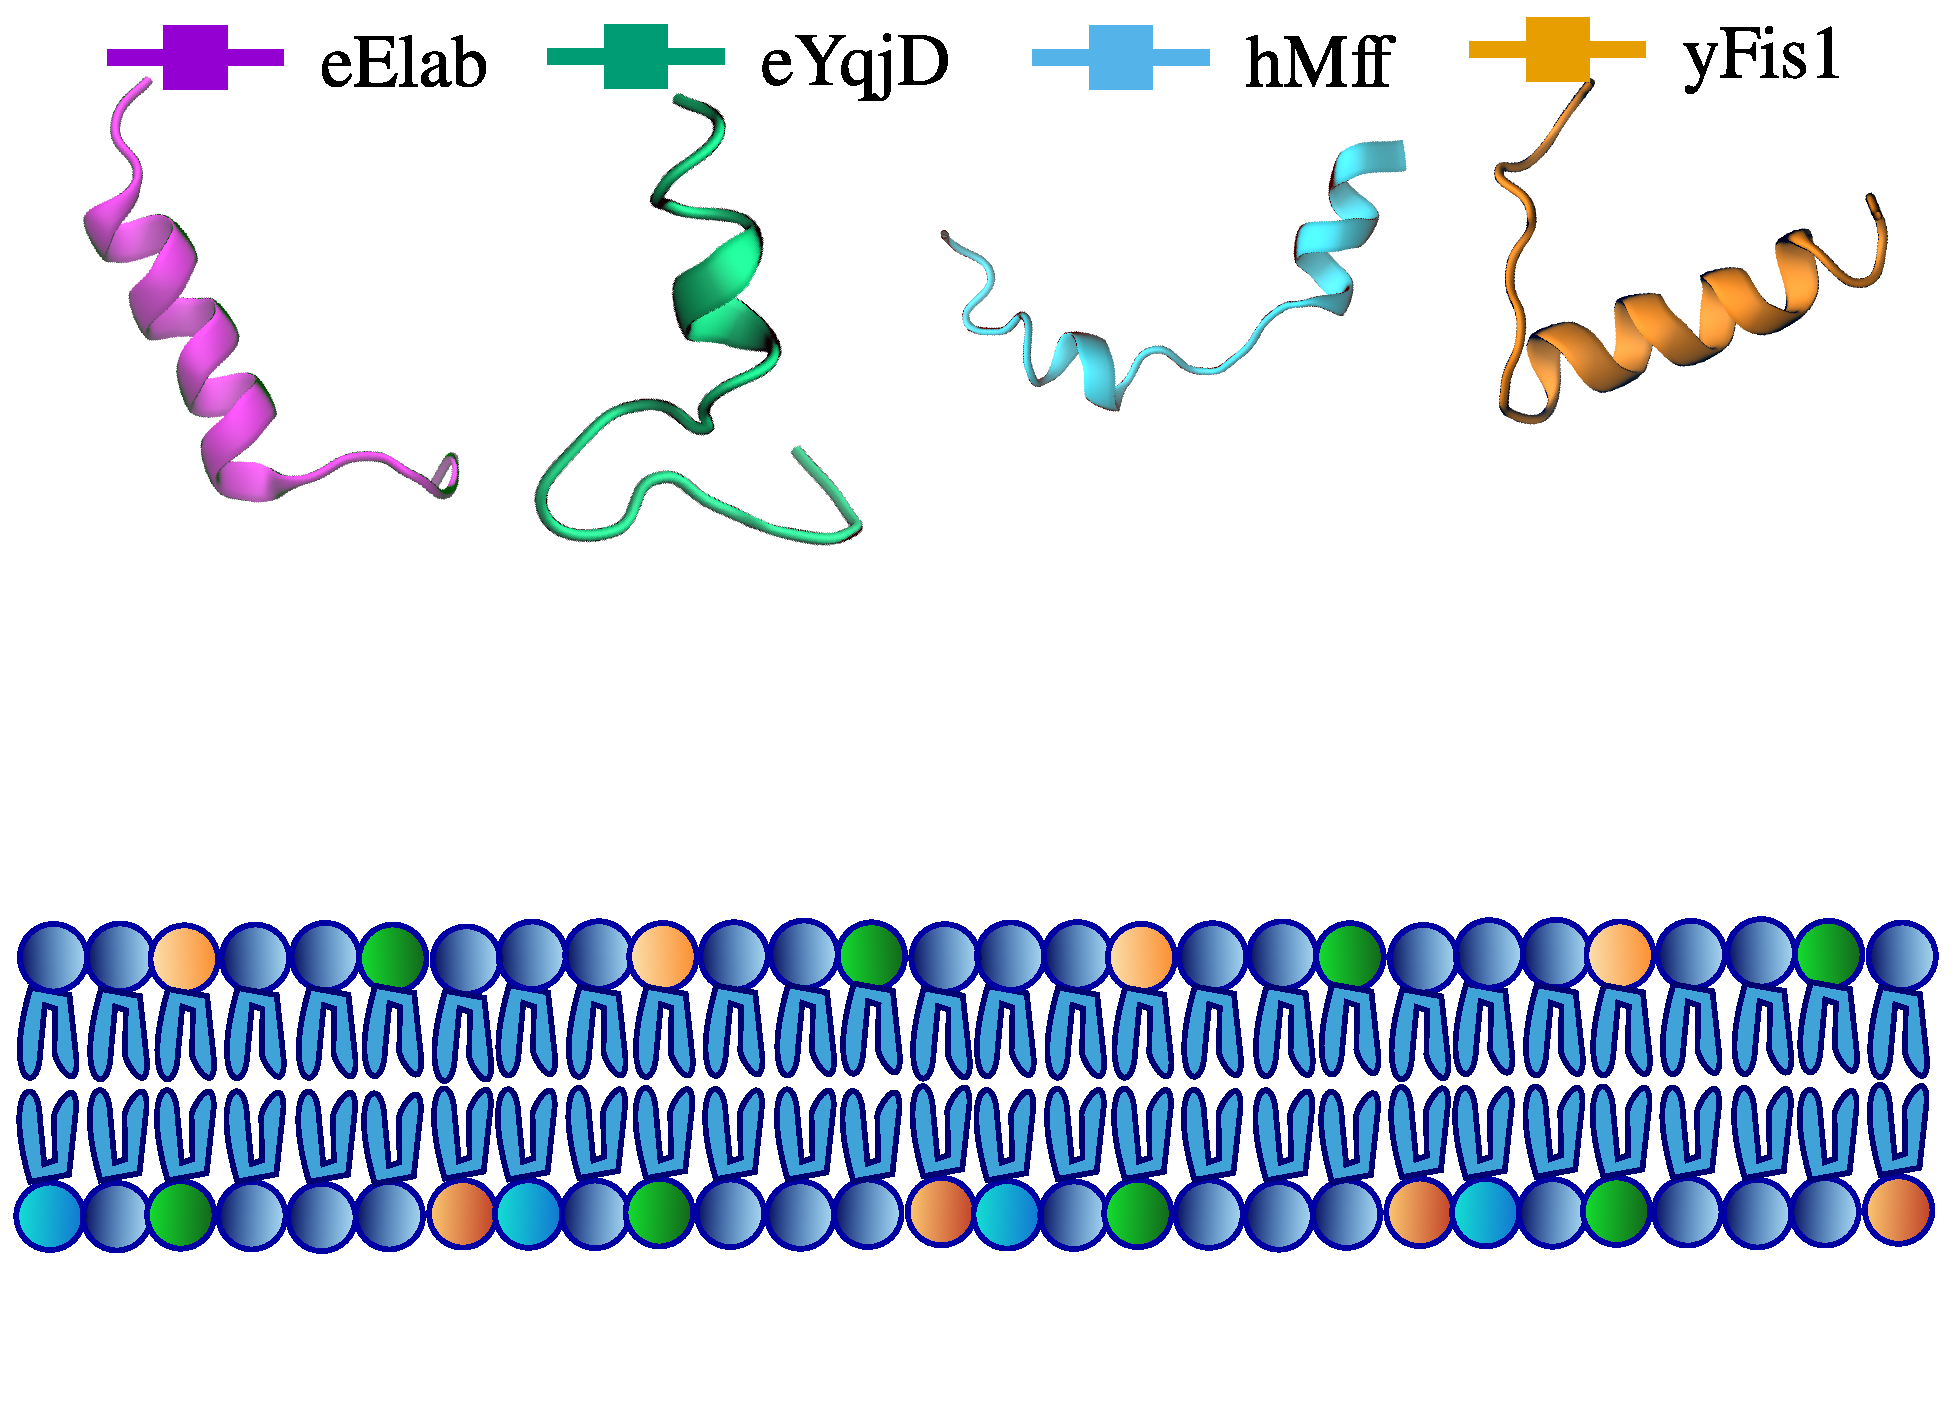
\includegraphics[height=5cm]{tail3.pdf}
\end{frame}



\addtocounter{framenumber}{-1}
\begin{frame}
\centering
\Large
Studied peptides\\

\vspace{0.3cm}

\resizebox{\textwidth}{!}{
\begin{tabular}{l l }
\hline
E.coli - ElaB & \texttt{PWQGIGVG\textcolor{red}{A}AVG\textcolor{red}{L}V\textcolor{red}{L}G\textcolor{red}{L}LL\textcolor{red}{A}RR} \\
E.coli - YqjD & \texttt{WT\textcolor{red}{G}VGIG\textcolor{red}{A}AIGVV\textcolor{red}{L}GVL\textcolor{red}{L}SRR}  \\
human - Mff & \texttt{\textcolor{red}{A}KREMVMISITV\textcolor{red}{A}FWL\textcolor{red}{L}NSW\textcolor{red}{L}WFRR}  \\
yeast - Fis1 & \texttt{\textcolor{red}{L}KGVVV\textcolor{red}{A}GGVL\textcolor{red}{A}GAVAV\textcolor{red}{A}SFF\textcolor{red}{L}RNKRR}  \\
\hline
Model - GWALP & \texttt{Ac-GG\textcolor{red}{A}LWL\textcolor{red}{A}LAL\textcolor{red}{A}LAL\textcolor{red}{A}LALWL\textcolor{red}{A}GA-NH-CH$_2$-CH$_2$OH}  \\
Model - Magainin 2 & \texttt{GIGKF\textcolor{red}{L}HS\textcolor{red}{A}KK\textcolor{red}{F}GK\textcolor{red}{A}F\textcolor{red}{V}GEIMNS } \\
\hline
\end{tabular}
}

\vspace{0.3cm}

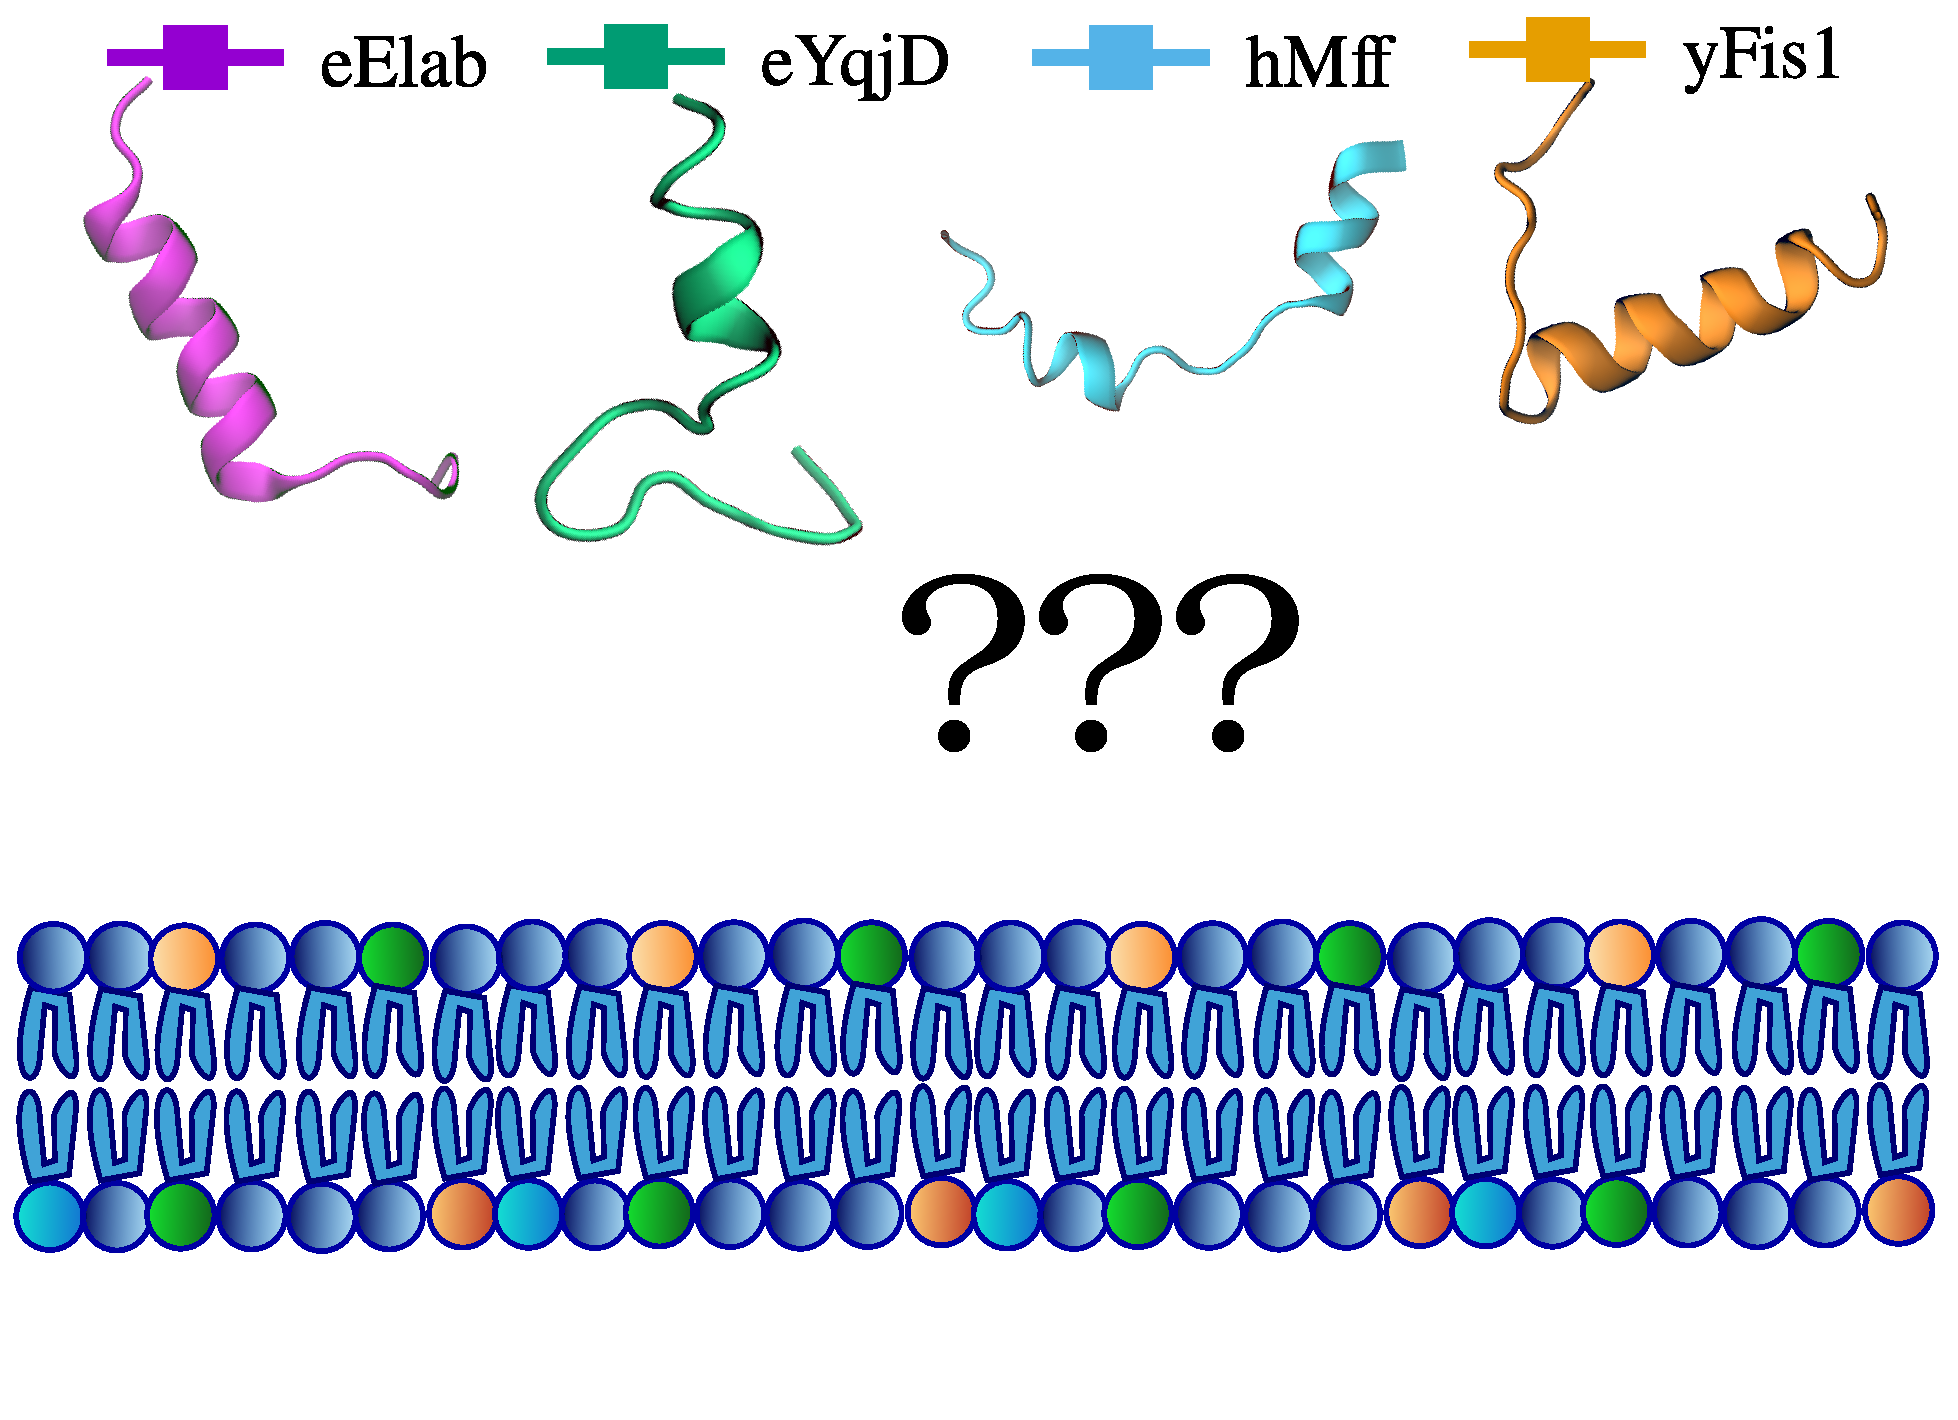
\includegraphics[height=5cm]{tail2.pdf}
\end{frame}



\addtocounter{framenumber}{-1}
\begin{frame}
\centering
\Large
Studied peptides\\

\vspace{0.3cm}

\resizebox{\textwidth}{!}{
\begin{tabular}{l l }
\hline
E.coli - ElaB & \texttt{PWQGIGVG\textcolor{red}{A}AVG\textcolor{red}{L}V\textcolor{red}{L}G\textcolor{red}{L}LL\textcolor{red}{A}RR} \\
E.coli - YqjD & \texttt{WT\textcolor{red}{G}VGIG\textcolor{red}{A}AIGVV\textcolor{red}{L}GVL\textcolor{red}{L}SRR}  \\
human - Mff & \texttt{\textcolor{red}{A}KREMVMISITV\textcolor{red}{A}FWL\textcolor{red}{L}NSW\textcolor{red}{L}WFRR}  \\
yeast - Fis1 & \texttt{\textcolor{red}{L}KGVVV\textcolor{red}{A}GGVL\textcolor{red}{A}GAVAV\textcolor{red}{A}SFF\textcolor{red}{L}RNKRR}  \\
\hline
Model - GWALP & \texttt{Ac-GG\textcolor{red}{A}LWL\textcolor{red}{A}LAL\textcolor{red}{A}LAL\textcolor{red}{A}LALWL\textcolor{red}{A}GA-NH-CH$_2$-CH$_2$OH}  \\
Model - Magainin 2 & \texttt{GIGKF\textcolor{red}{L}HS\textcolor{red}{A}KK\textcolor{red}{F}GK\textcolor{red}{A}F\textcolor{red}{V}GEIMNS } \\
\hline
\end{tabular}
}

\vspace{0.3cm}

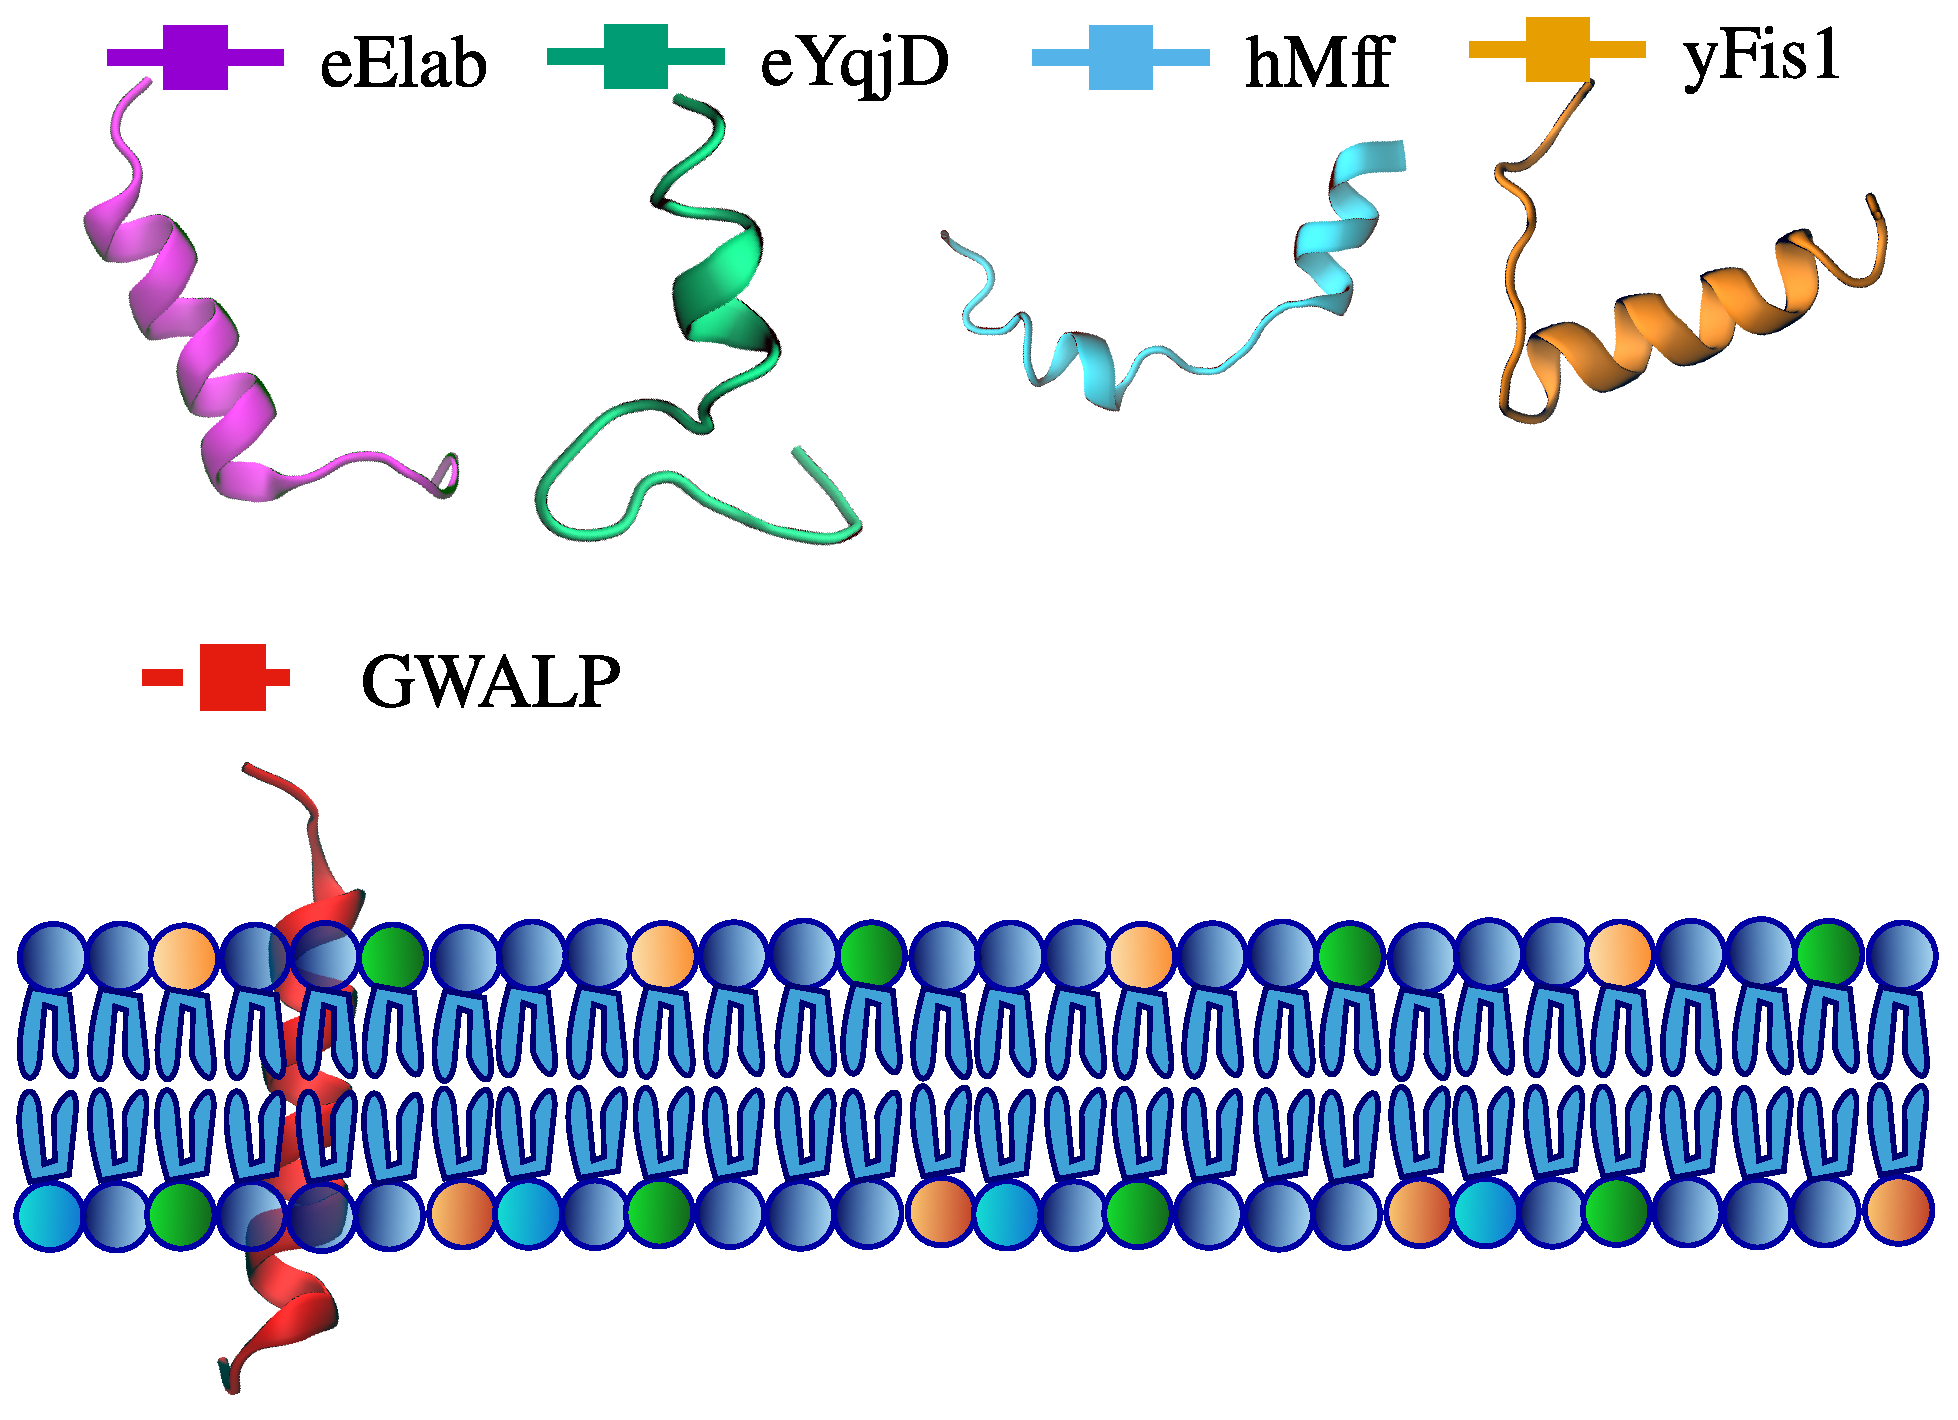
\includegraphics[height=5cm]{tail1.pdf}
\end{frame}





\addtocounter{framenumber}{-1}
\begin{frame}
\centering
\Large
Studied peptides\\

\vspace{0.3cm}

\resizebox{\textwidth}{!}{
\begin{tabular}{l l }
\hline
E.coli - ElaB & \texttt{PWQGIGVG\textcolor{red}{A}AVG\textcolor{red}{L}V\textcolor{red}{L}G\textcolor{red}{L}LL\textcolor{red}{A}RR} \\
E.coli - YqjD & \texttt{WT\textcolor{red}{G}VGIG\textcolor{red}{A}AIGVV\textcolor{red}{L}GVL\textcolor{red}{L}SRR}  \\
human - Mff & \texttt{\textcolor{red}{A}KREMVMISITV\textcolor{red}{A}FWL\textcolor{red}{L}NSW\textcolor{red}{L}WFRR}  \\
yeast - Fis1 & \texttt{\textcolor{red}{L}KGVVV\textcolor{red}{A}GGVL\textcolor{red}{A}GAVAV\textcolor{red}{A}SFF\textcolor{red}{L}RNKRR}  \\
\hline
Model - GWALP & \texttt{Ac-GG\textcolor{red}{A}LWL\textcolor{red}{A}LAL\textcolor{red}{A}LAL\textcolor{red}{A}LALWL\textcolor{red}{A}GA-NH-CH$_2$-CH$_2$OH}  \\
Model - Magainin 2 & \texttt{GIGKF\textcolor{red}{L}HS\textcolor{red}{A}KK\textcolor{red}{F}GK\textcolor{red}{A}F\textcolor{red}{V}GEIMNS } \\
\hline
\end{tabular}
}

\vspace{0.3cm}

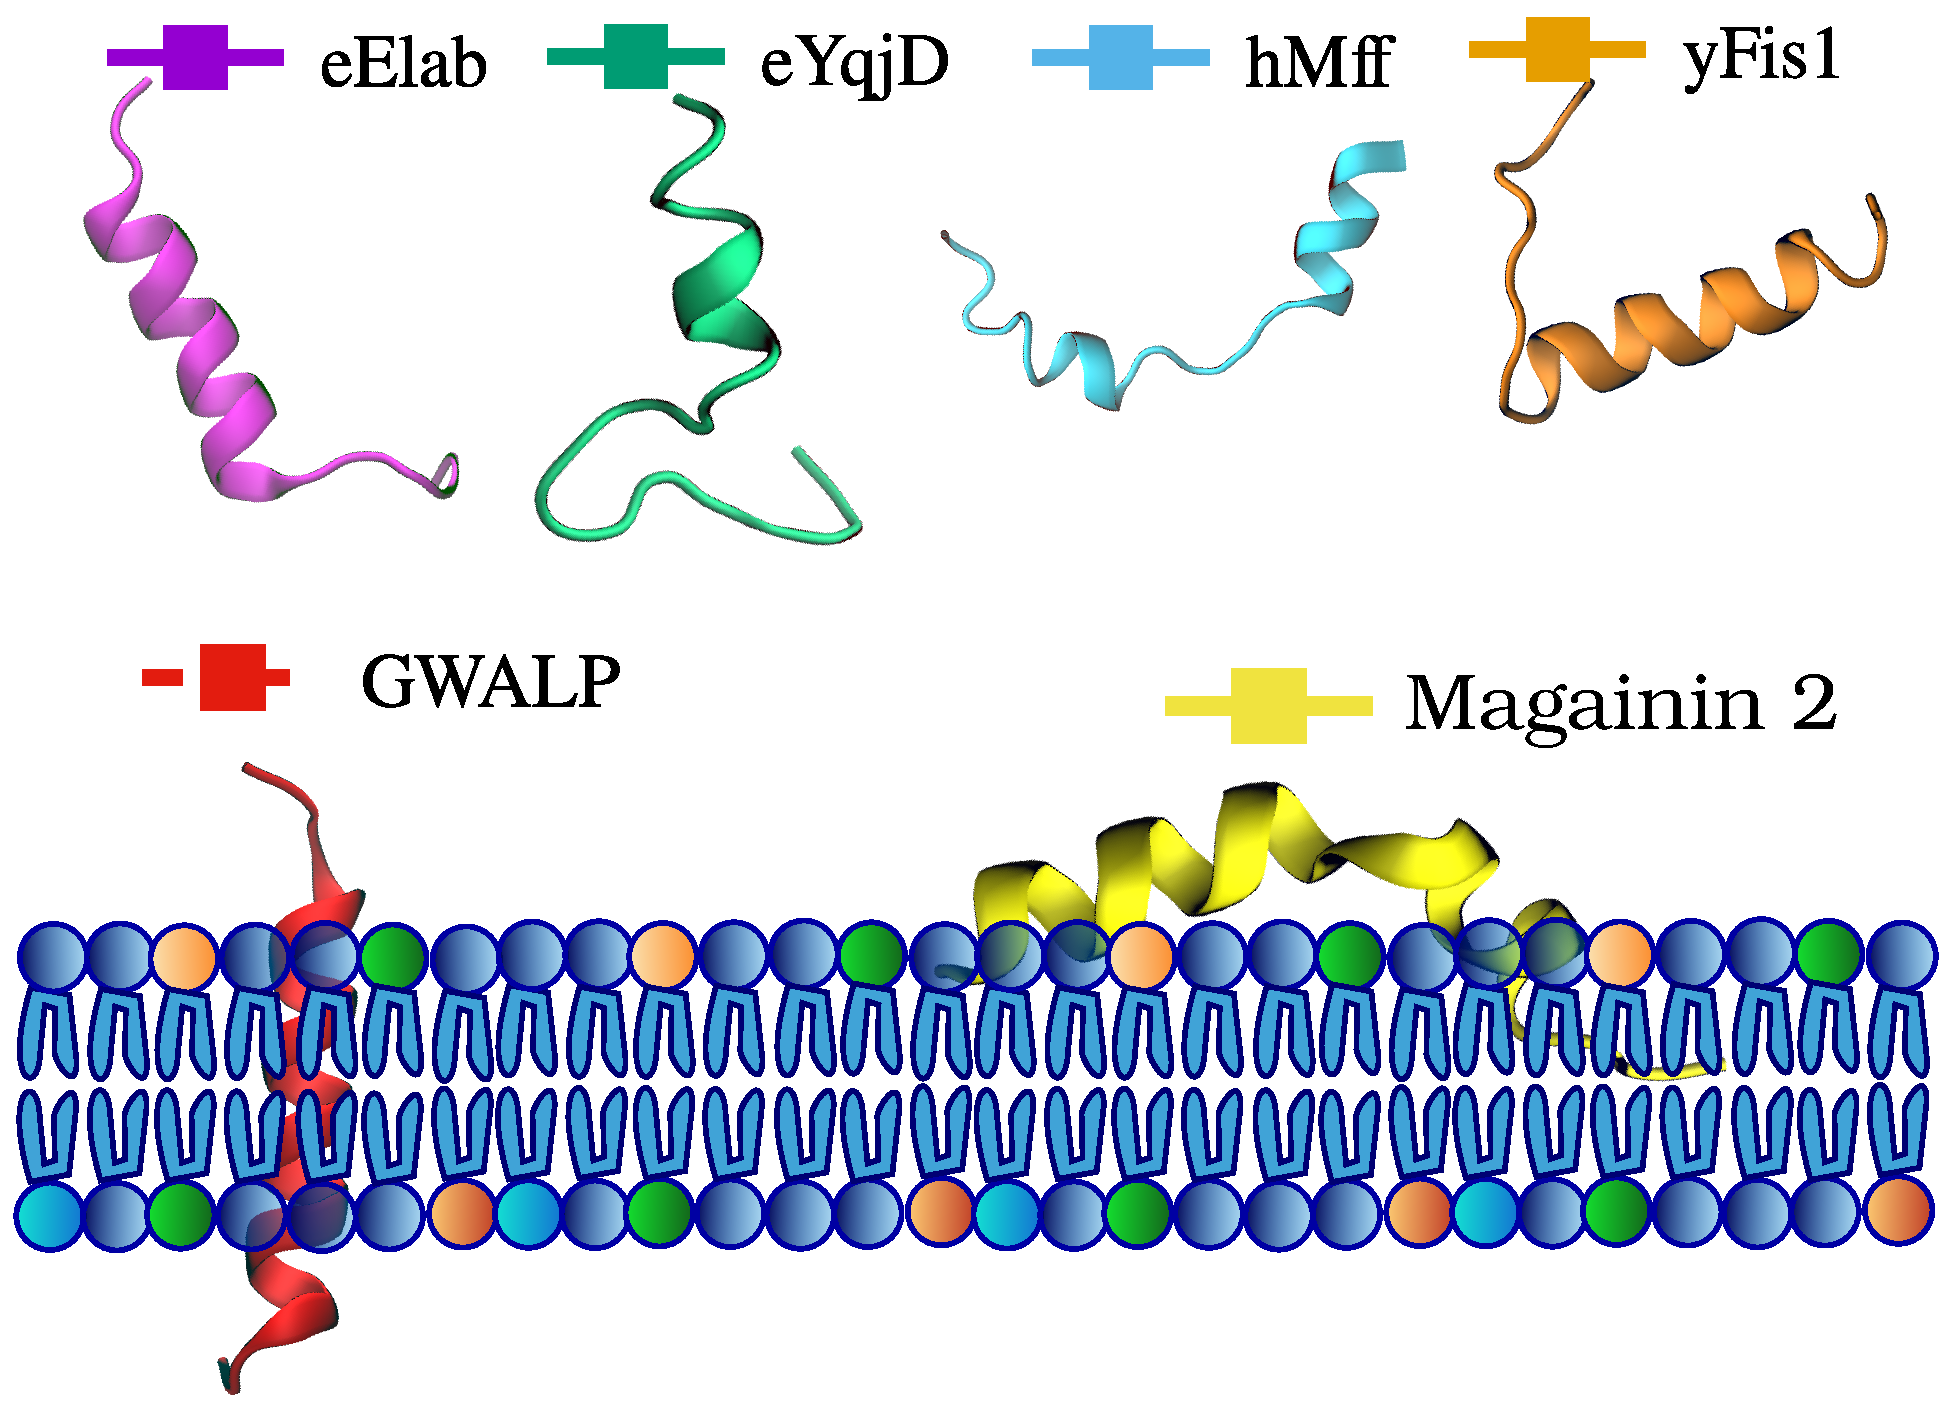
\includegraphics[height=5cm]{tail0.pdf}
\end{frame}


\begin{frame}


\centering

\Large

Studied peptides\\

\vspace{0.3cm}


\resizebox{\textwidth}{!}{

\begin{tabular}{l l r r r r}

\ & \ &  \textcolor{OliveGreen}{Hydrobphobic} & \textcolor{red}{Acid} & \textcolor{blue}{Basic} & \textcolor{black}{Neutral} \\

\hline

E.coli - ElaB & \texttt{\textcolor{OliveGreen}{PW}Q\textcolor{OliveGreen}{GIGVGAAVGLVLGLLLA}\textcolor{blue}{RR}} & \textcolor{OliveGreen}{63.64\%} & \textcolor{red}{0.0\%} & \textcolor{blue}{9.09\%} & 27.27\% \\


E.coli - YqjD & \texttt{\textcolor{OliveGreen}{W}T\textcolor{OliveGreen}{GVGIGAAIGVVLGVLL}S\textcolor{blue}{RR}} & \textcolor{OliveGreen}{57.14\%} & \textcolor{red}{0.0\%} & \textcolor{blue}{9.52\%} & 33.33\% \\


human - Mff & \texttt{\textcolor{OliveGreen}{A}\textcolor{blue}{KR}\textcolor{red}{E}\textcolor{OliveGreen}{MVM}IS\textcolor{OliveGreen}{I}T\textcolor{OliveGreen}{VAFWLL}NS\textcolor{OliveGreen}{WLWF}\textcolor{blue}{RR}} & \textcolor{OliveGreen}{60.00\%} & \textcolor{red}{4.0\%} & \textcolor{blue}{16.00\%} & 20.00\% \\



yeast - Fis1 & \texttt{\textcolor{OliveGreen}{L}\textcolor{blue}{K}\textcolor{OliveGreen}{GVVVAGGVLAGAVAVA}S\textcolor{OliveGreen}{FFL}\textcolor{blue}{R}N\textcolor{blue}{KRR}} & \textcolor{OliveGreen}{59.26\%} & \textcolor{red}{0.0\%} & \textcolor{blue}{18.52\%} & 22.22\% \\








\hline


Model - GWALP & \texttt{Ac-\textcolor{OliveGreen}{GGALWLALALALALALALWLAGA}-NH-CH$_2$-CH$_2$OH } & \textcolor{OliveGreen}{100.00\%} & \textcolor{red}{0.0\%} & \textcolor{blue}{0.00\%} & 0.00\% \\


Model - Magainin 2 & \texttt{\textcolor{OliveGreen}{GIG}\textcolor{blue}{K}\textcolor{OliveGreen}{FL}\textcolor{blue}{H}S\textcolor{OliveGreen}{A}\textcolor{blue}{KK}\textcolor{OliveGreen}{FG}\textcolor{blue}{K}\textcolor{OliveGreen}{AFVG}\textcolor{red}{E}\textcolor{OliveGreen}{IM}NS } & \textcolor{OliveGreen}{43.48\%} & \textcolor{red}{4.4\%} & \textcolor{blue}{21.74\%} & 30.43\% \\

\hline

\end{tabular}

}


{\tiny https://www.peptide2.com/N\_peptide\_hydrophobicity\_hydrophilicity.php}

\vspace{0.2cm}

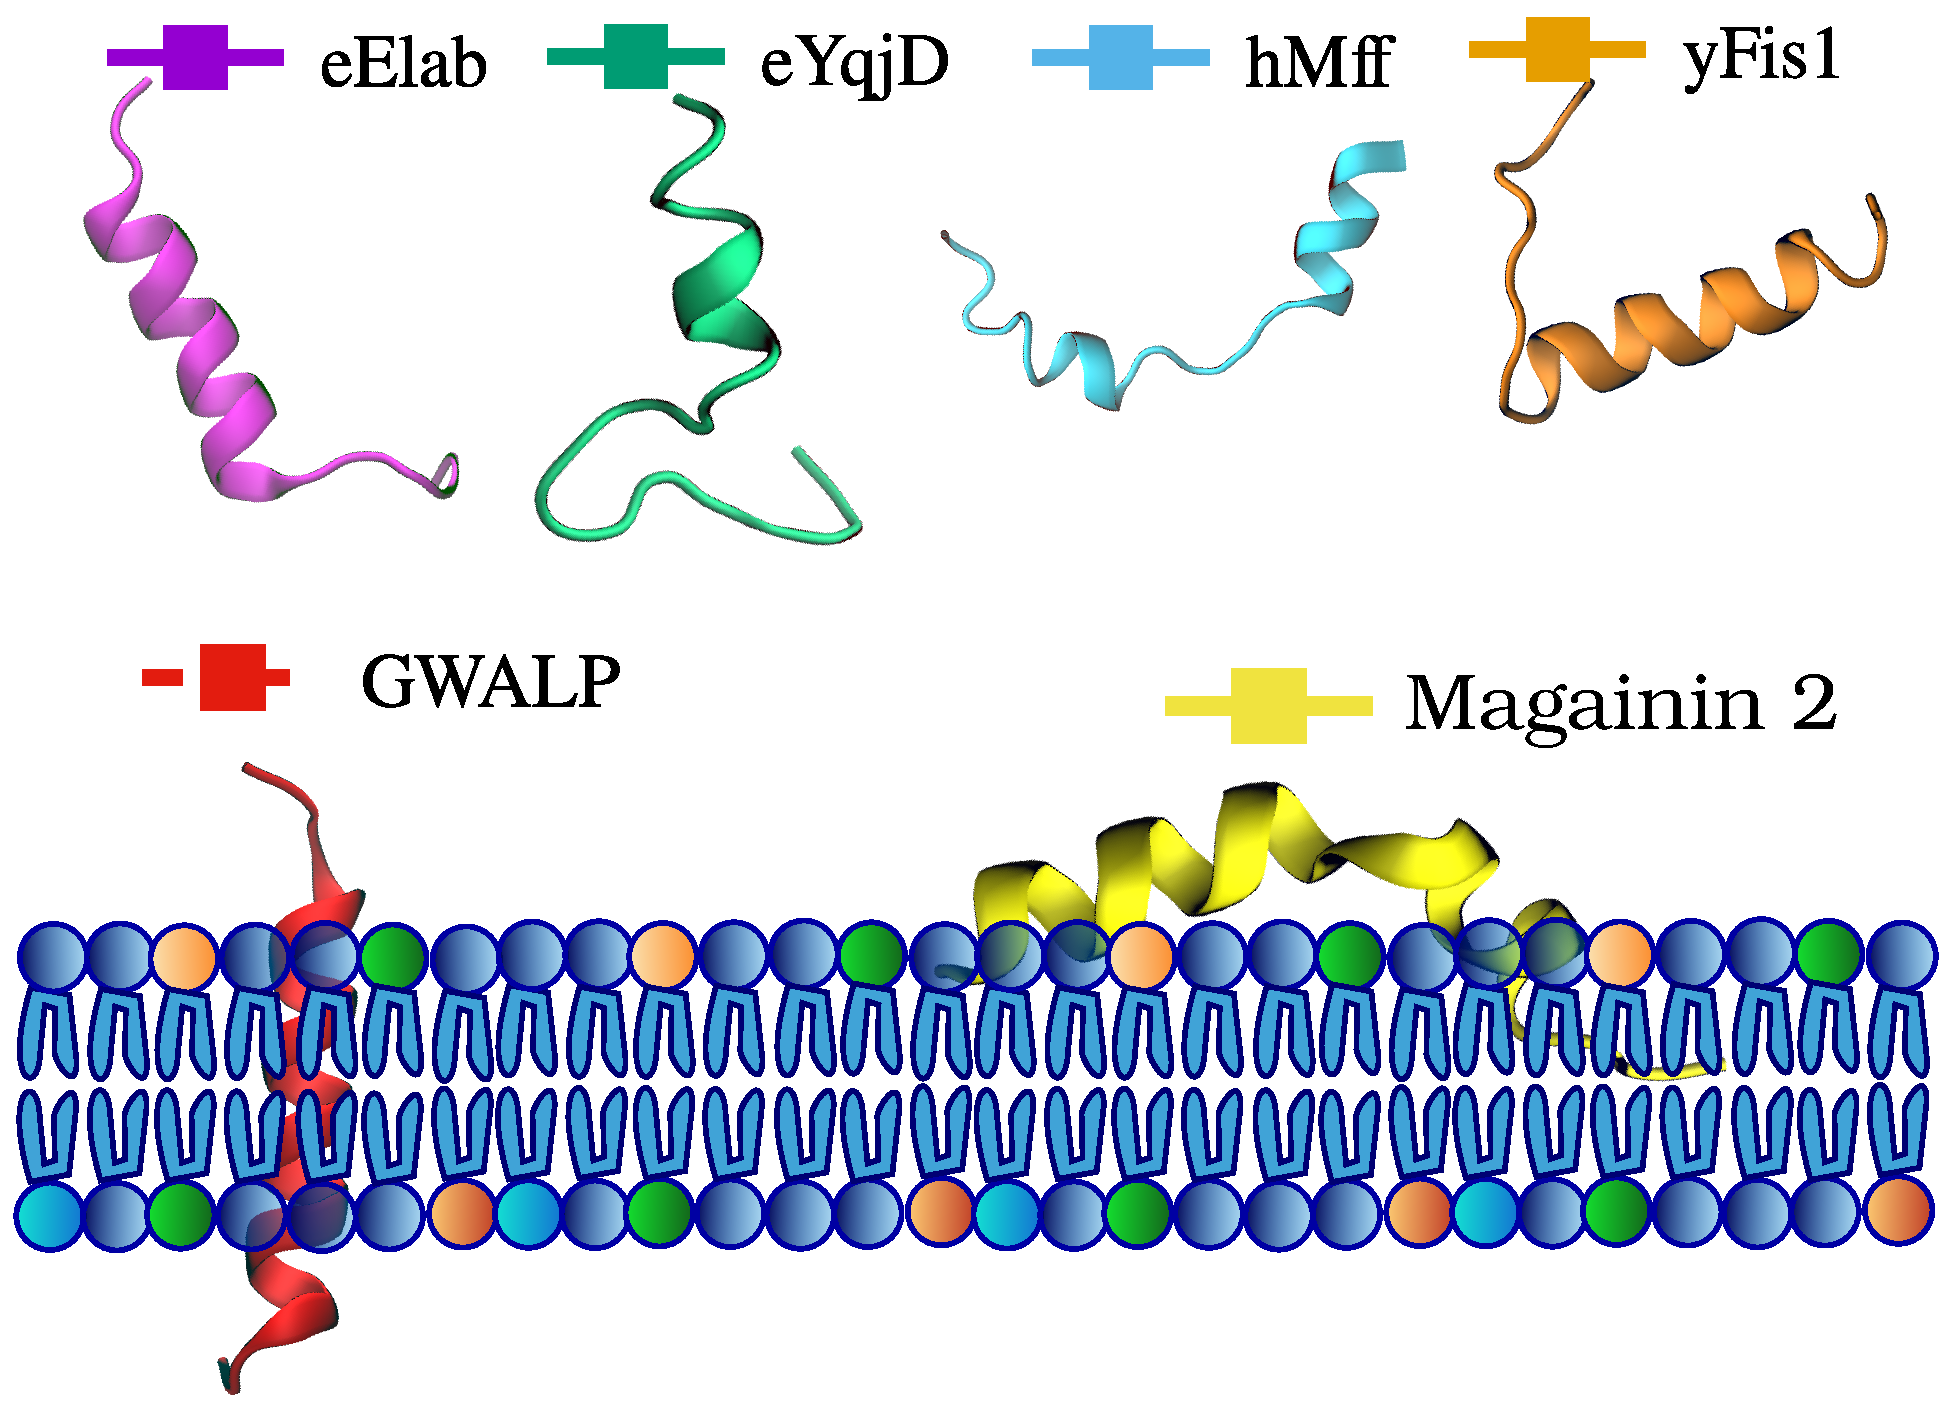
\includegraphics[height=4.5cm]{tail0.pdf}

\end{frame}


\subsection{Experimental results}

\begin{frame}
\begin{center}
\Large{\centering
\textbf{Results} \\}

\vspace{0.5cm}

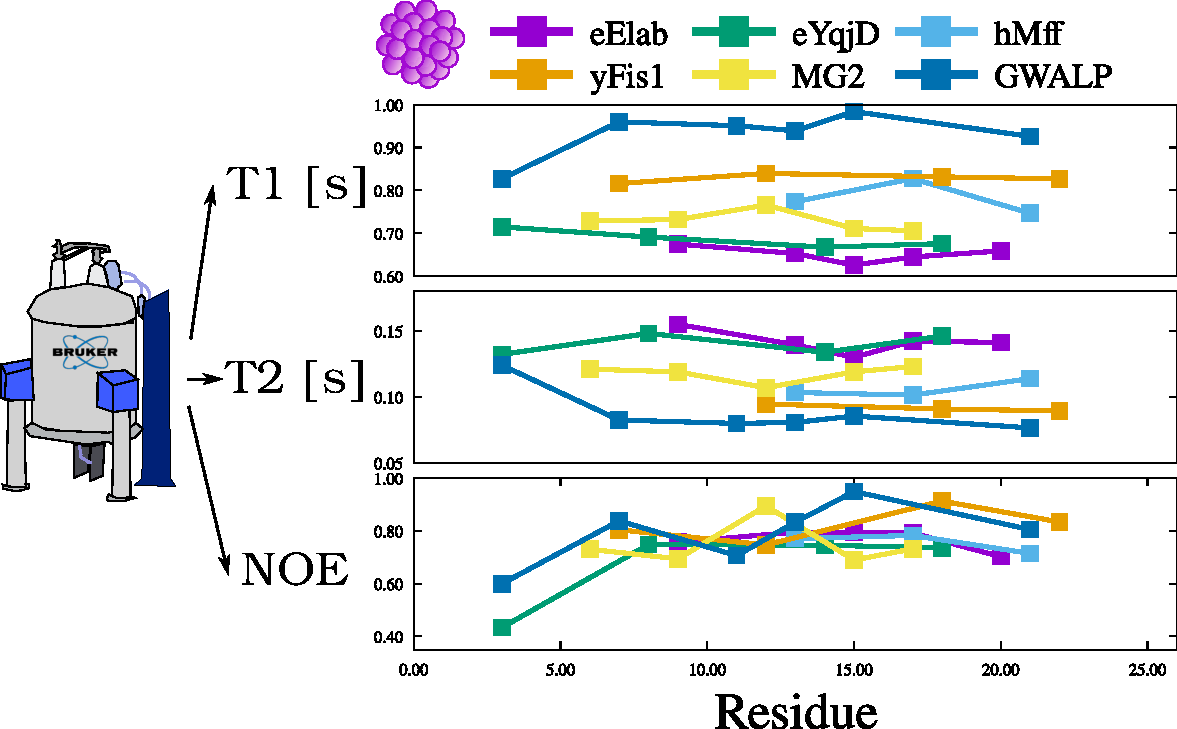
\includegraphics[height=6.5cm]{relax_exp1.pdf}
\end{center}
\end{frame}

\addtocounter{framenumber}{-1}
\begin{frame}
\begin{center}

\Large{\centering
\textbf{Results} \\}

\vspace{0.5cm}

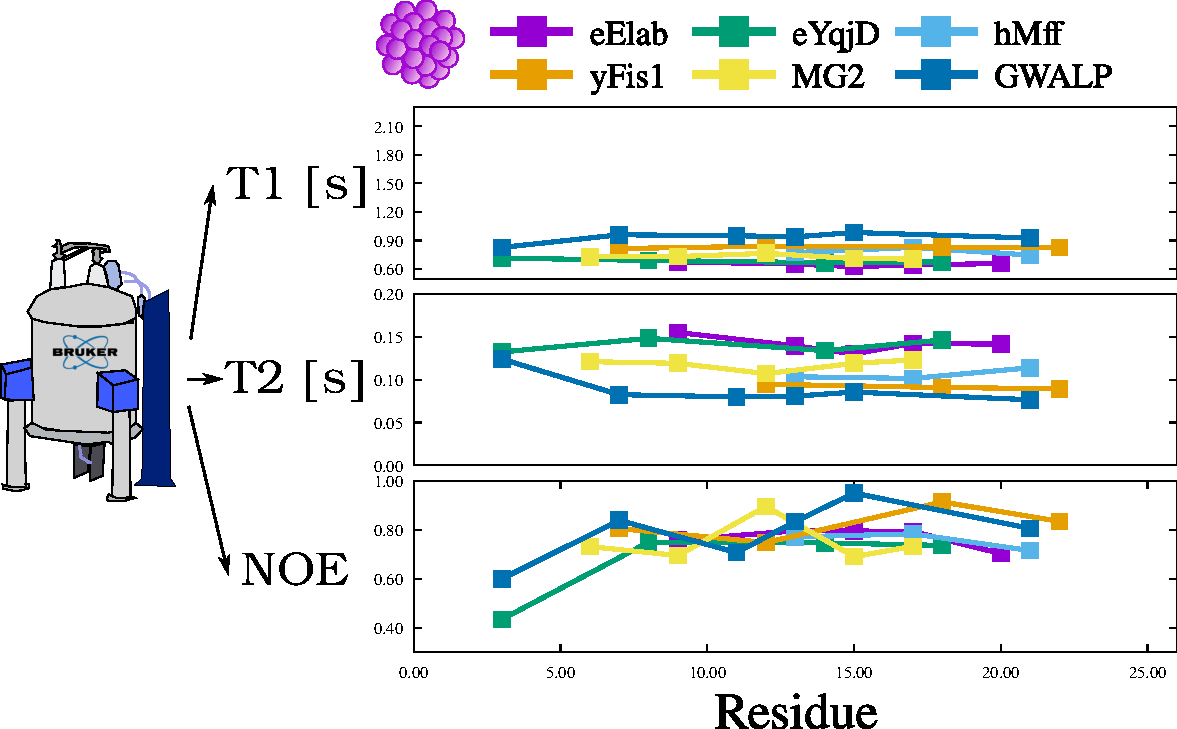
\includegraphics[height=6.5cm]{relax_exp2.pdf}
\end{center}
\end{frame}

\addtocounter{framenumber}{-1}
\begin{frame}
\begin{center}
\Large{\centering
\textbf{Results} \\}

\vspace{0.5cm}

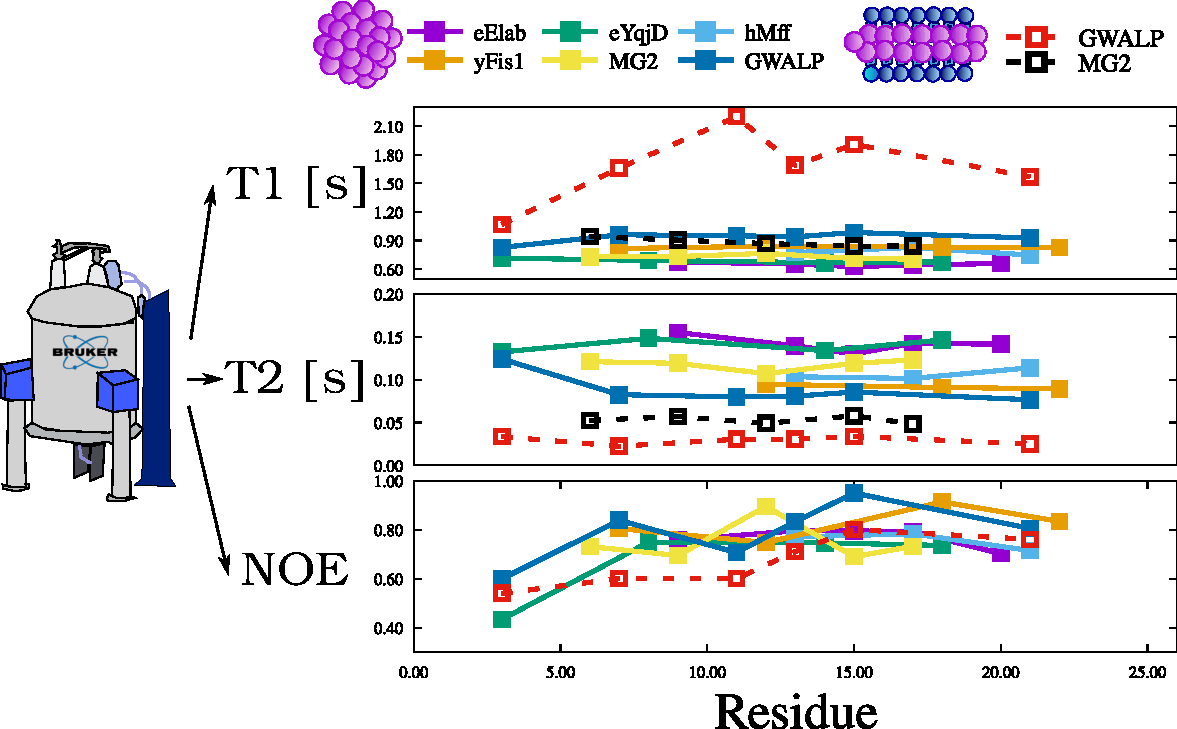
\includegraphics[height=6.5cm]{relax_exp3.pdf}
\end{center}
\end{frame}

\subsection{Redfield}


\begin{frame}
\LARGE{\centering
\textbf{How can we interpret experimental NMR spin relaxation times?} \\}

To be developed or deleted, comment on what people do otherwise...

\begin{center}
 \includegraphics[height=5cm]{kolo.png}
\end{center}


\end{frame}



\begin{frame}
\begin{center}
\Large{\centering
\textbf{How can we interpret experimental NMR spin relaxation times?} \\}

\vspace{0.5cm}


\includegraphics[height=6cm]{redfield1.pdf}
\end{center}
\end{frame}


\addtocounter{framenumber}{-1}
\begin{frame}
\begin{center}
\Large{\centering
\textbf{How can we interpret experimental NMR spin relaxation times?} \\}

\vspace{0.5cm}

\includegraphics[height=6cm]{redfield2.pdf}
\end{center}
\end{frame}

\addtocounter{framenumber}{-1}
\begin{frame}
\begin{center}
\Large{\centering

\textbf{How can we interpret experimental NMR spin relaxation times?} \\}

\vspace{0.5cm}


\includegraphics[height=6cm]{redfield3.pdf}
\end{center}
\end{frame}


\addtocounter{framenumber}{-1}
\begin{frame}
\begin{center}
\Large{\centering

\textbf{How can we interpret experimental NMR spin relaxation times?} \\}

\vspace{0.5cm}


\includegraphics[height=6cm]{redfield4.pdf}
\end{center}
\end{frame}


\addtocounter{framenumber}{-1}
\begin{frame}
\begin{center}
\Large{\centering

\textbf{How can we interpret experimental NMR spin relaxation times?} \\}

\vspace{0.5cm}


\includegraphics[height=6cm]{redfield5.pdf}
\end{center}
\end{frame}

\addtocounter{framenumber}{-1}
\begin{frame}
\begin{center}
\Large{\centering

\textbf{How can we interpret experimental NMR spin relaxation times?} \\}

\vspace{0.5cm}


\includegraphics[height=6cm]{redfield56.pdf}
\end{center}
\end{frame}

\addtocounter{framenumber}{-1}
\begin{frame}
\begin{center}
\Large{\centering

\textbf{How can we interpret experimental NMR spin relaxation times?} \\}

\vspace{0.5cm}


\includegraphics[height=6cm]{redfield6.pdf}
\end{center}
\end{frame}


\addtocounter{framenumber}{-1}
\begin{frame}
\begin{center}
\Large{\centering

\textbf{How can we interpret experimental NMR spin relaxation times?} \\}

\vspace{0.5cm}


\includegraphics[height=6cm]{redfield7.pdf}
\end{center}
\end{frame}

\section{MD results}

\begin{frame}
\LARGE{\centering
\textbf{Results} \\

}


\end{frame}

\subsection{Empty micelles}

\begin{frame}
\begin{center}
\Large{\centering

\textbf{Empty SDS micelles} \\}

\vspace{0.5cm}


\includegraphics[height=6cm]{sds7.pdf}
\end{center}
\end{frame}



\addtocounter{framenumber}{-1}
\begin{frame}
\begin{center}
\Large{\centering

\textbf{Empty SDS micelles} \\}

\vspace{0.5cm}


\includegraphics[height=6cm]{sds9.pdf}
\end{center}
\end{frame}



\addtocounter{framenumber}{-1}
\begin{frame}
\begin{center}
\Large{\centering

\textbf{Empty SDS micelles} \\}

\vspace{0.5cm}


\includegraphics[height=6cm]{sds8.pdf}
\end{center}
\end{frame}





\addtocounter{framenumber}{-1}
\begin{frame}
\begin{center}
\Large{\centering

\textbf{Empty SDS micelles} \\}

\vspace{0.5cm}


\includegraphics[height=6cm]{sds5.pdf}
\end{center}
\end{frame}

\addtocounter{framenumber}{-1}
\begin{frame}
\begin{center}
\Large{\centering

\textbf{Empty SDS micelles} \\}

\vspace{0.5cm}


\includegraphics[height=6cm]{sds4.pdf}
\end{center}
\end{frame}


\addtocounter{framenumber}{-1}
\begin{frame}
\begin{center}
\Large{\centering

\textbf{Empty SDS micelles} \\}

\vspace{0.5cm}


\includegraphics[height=6cm]{sds3.pdf}
\end{center}
\end{frame}


\addtocounter{framenumber}{-1}
\begin{frame}
\begin{center}
\Large{\centering

\textbf{Empty SDS micelles} \\}

\vspace{0.5cm}


\includegraphics[height=6cm]{sds2.pdf}
\end{center}
\end{frame}


\addtocounter{framenumber}{-1}
\begin{frame}
\begin{center}
\Large{\centering

\textbf{Empty SDS micelles} \\}

\vspace{0.5cm}


\includegraphics[height=6cm]{sds1.pdf}
\end{center}
\end{frame}


\addtocounter{framenumber}{-1}
\begin{frame}
\begin{center}
\Large{\centering

\textbf{Empty SDS micelles} \\}

\vspace{0.5cm}


\includegraphics[height=6cm]{sds0.pdf}
\end{center}
\end{frame}


\subsection{Mag2}


\begin{frame}
\begin{center}
\Large{\centering

\textbf{Optimization of simulations} \\}

\vspace{0.5cm}


\includegraphics[height=5cm]{mag5.pdf}
\end{center}
\end{frame}

\addtocounter{framenumber}{-1}
\begin{frame}
\begin{center}
\Large{\centering

\textbf{Optimization of simulations} \\}

\vspace{0.5cm}


\includegraphics[height=5cm]{mag4.pdf}
\end{center}
\end{frame}


\addtocounter{framenumber}{-1}
\begin{frame}
\begin{center}
\Large{\centering

\textbf{Optimization of simulations} \\}

\vspace{0.5cm}


\includegraphics[height=5cm]{mag3.pdf}
\end{center}
\end{frame}


\addtocounter{framenumber}{-1}
\begin{frame}
\begin{center}
\Large{\centering

\textbf{Optimization of simulations} \\}

\vspace{0.5cm}


\includegraphics[height=5cm]{mag2.pdf}
\end{center}
\end{frame}


\addtocounter{framenumber}{-1}
\begin{frame}
\begin{center}
\Large{\centering

\textbf{Optimization of simulations} \\}

\vspace{0.5cm}


\includegraphics[height=5cm]{mag1.pdf}
\end{center}
\end{frame}






\begin{frame}
\begin{center}


\vspace{0.5cm}


\includegraphics[height=7cm]{all_pep8.pdf}
\end{center}
\end{frame}




\addtocounter{framenumber}{-1}
\begin{frame}
\begin{center}


\vspace{0.5cm}


\includegraphics[height=7cm]{all_pep7.pdf}
\end{center}
\end{frame}

\addtocounter{framenumber}{-1}
\begin{frame}
\begin{center}


\vspace{0.5cm}


\includegraphics[height=7cm]{all_pep6.pdf}
\end{center}
\end{frame}

\addtocounter{framenumber}{-1}
\begin{frame}
\begin{center}


\vspace{0.5cm}


\includegraphics[height=7cm]{all_pep5.pdf}
\end{center}
\end{frame}

\addtocounter{framenumber}{-1}
\begin{frame}
\begin{center}


\vspace{0.5cm}


\includegraphics[height=7cm]{all_pep4.pdf}
\end{center}
\end{frame}


\addtocounter{framenumber}{-1}
\begin{frame}
\begin{center}


\vspace{0.5cm}


\includegraphics[height=7cm]{all_pep3.pdf}
\end{center}
\end{frame}


\addtocounter{framenumber}{-1}
\begin{frame}
\begin{center}


\vspace{0.5cm}


\includegraphics[height=7cm]{all_pep2.pdf}
\end{center}
\end{frame}


\addtocounter{framenumber}{-1}
\begin{frame}
\begin{center}


\vspace{0.5cm}


\includegraphics[height=7cm]{all_pep1.pdf}
\end{center}
\end{frame}


\addtocounter{framenumber}{-1}
\begin{frame}
\begin{center}


\vspace{0.5cm}


\includegraphics[height=7cm]{all_pep9.pdf}
\end{center}
\end{frame}



\addtocounter{framenumber}{-1}
\begin{frame}
\begin{center}


\vspace{0.5cm}


\includegraphics[height=7cm]{all_pep10.pdf}
\end{center}
\end{frame}


\addtocounter{framenumber}{-1}
\begin{frame}
\begin{center}


\vspace{0.5cm}


\includegraphics[height=7cm]{all_pep11.pdf}
\end{center}
\end{frame}


\addtocounter{framenumber}{-1}
\begin{frame}
\begin{center}


\vspace{0.5cm}


\includegraphics[height=7cm]{all_pep12.pdf}
\end{center}
\end{frame}


\addtocounter{framenumber}{-1}
\begin{frame}
\begin{center}


\vspace{0.5cm}


\includegraphics[height=7cm]{all_pep13.pdf}
\end{center}
\end{frame}


\addtocounter{framenumber}{-1}
\begin{frame}
\begin{center}


\vspace{0.5cm}


\includegraphics[height=7cm]{all_pep14.pdf}
\end{center}
\end{frame}


\begin{frame}
\LARGE{\centering
\textbf{Results in Micelles} \\
Empty bicelles work with CHARMM36 and OPC water \\
Optimization of micelle size\\
GWALP fits better as dimer\\


\vspace{1.5cm}

to be developed
}


\end{frame}


\begin{frame}
\LARGE{\centering
\textbf{Results in Micelles} \\
We can get time scales\\
Comment on helicity??


\vspace{1.5cm}

to be developed
}


\end{frame}



\begin{frame}
\LARGE{\centering
\textbf{Acknowledgmnents} \\


\vspace{1.5cm}

to be developed
}


\end{frame}

%----------------------------------------------------------------------------------------

\end{document} 